\documentclass[a4paper, 11pt]{report} % Font size (can be 10pt, 11pt or 12pt) and paper size (remove a4paper for US letter paper)
\usepackage[italian]{babel}      							% Lingua italiana
\usepackage[margin=.9in]{geometry}             % Imposta i margini del documento

\usepackage[T1]{fontenc} % Required for accented characters
\usepackage[mathletters]{ucs}    % Caratteri matematici come UTF8
\usepackage[utf8,utf8x]{inputenc}      % Ancora utf8

\usepackage{eurosym}                %simbolo dell'euro
\usepackage{listings}
\usepackage[usenames,dvipsnames,svgnames,table]{xcolor}
% Imposta lo spazio nella list of listing in modo simile alla list of figures/tables
%\makeatletter
%\let\my@chapter\@chapter
%\renewcommand*{\@chapter}{%
%  \addtocontents{lol}{\protect\addvspace{10pt}}%
%  \my@chapter}
%\makeatother


\definecolor{codegreen}{rgb}{0,0.6,0}
\definecolor{codegray}{rgb}{0.5,0.5,0.5}
\definecolor{backcolor}{rgb}{0.98,0.98,0.98}

\renewcommand{\lstlistingname}{Codice}% Listing -> codice
\renewcommand{\lstlistlistingname}{Elenco dei frammenti di codice}% List of Listings -> Frammenti di codice

\lstdefinestyle{mystyle}{
    backgroundcolor=\color{backcolor},   
    commentstyle=\color{Peach}\ttfamily,
    keywordstyle=\color{RoyalBlue},
    numberstyle=\tiny\color{codegray},
    stringstyle=\color{SeaGreen}\ttfamily,
    basicstyle=\footnotesize\ttfamily,
    breakatwhitespace=false,         
    breaklines=true,                 
    captionpos=b,                    
    keepspaces=true,                 
    numbers=left,                    
    numbersep=5pt,                  
    showspaces=false,                
    showstringspaces=false,
    showtabs=false,                  
    tabsize=2,
    frame=trbl, % draw a frame at the top, right, left and bottom of the listing
	frameround=ftff, % angolo in basso a destro curvo
	framesep=4pt, % quarter circle size of the round corners,
	inputencoding=utf8,
    extendedchars=true,
    literate={á}{{\'a}}1 {à}{{\`a}}1 {é}{{\'e}}1 {è}{{\`e}}1 {ù}{{\`u}}1 {ò}{{\`o}}1 {ì}{{\`i}}1,
    belowskip=1em,
    aboveskip=1em,
}

 
\lstset{style=mystyle}

\lstdefinelanguage{JavaScript}
{
  % list of keywords
  morekeywords={ true, false, catch, function, break,	new, class, extends, var, require, switch, return, import, if, while, for, this, View, Text, StyleSheet},
  sensitive=false, % keywords are not case-sensitive
  morecomment=[l]{//}, % l is for line comment
  morecomment=[s]{/*}{*/}, % s is for start and end delimiter
  morestring=[b]' % defines that strings are enclosed in double quotes
}

\lstdefinelanguage{JSON}
{
  % list of keywords
  morekeywords={string, boolean, int, Array, Node, Asset, AssetDetail, Filter, FilterItem},
  sensitive=false, % keywords are not case-sensitive
  morecomment=[l]{//}, % l is for line comment
  morecomment=[s]{/*}{*/}, % s is for start and end delimiter
  morestring=[b]" % defines that strings are enclosed in double quotes
}

\lstdefinelanguage{URM}
{
	% list of keywords
	morekeywords={ S, J, T, Z, I},
	sensitive=false, % keywords are not case-sensitive
	morecomment=[l]{//}, % l is for line comment
	morecomment=[s]{/*}{*/}, % s is for start and end delimiter
	morestring=[b]' % defines that strings are enclosed in double quotes
}

\lstdefinelanguage{RDFA}{
	language=html,
	sensitive=true, 
	alsoletter={<>=-},
	ndkeywords={
		% General
		=,
		% HTML attributes
		charset=, id=, width=, height=, property=, about=, rel=, rev=, prefix=, vocab=, content=, datatype=
	},  
	morecomment=[s]{<!--}{-->},
	tag=[s]
}

%\tightlist per compatibilità con pandoc
\providecommand{\tightlist}{%
	\setlength{\itemsep}{0pt}\setlength{\parskip}{0pt}}


\usepackage[labelfont=bf]{caption}

\usepackage[protrusion=true,expansion=true]{microtype} % Better typography
\usepackage{graphicx} % Required for including pictures
\usepackage{wrapfig} % Allows in-line images


\usepackage{subfig}
\usepackage{hyperref}
\usepackage{placeins}
\usepackage{sourcecodepro}
\usepackage{hyperref}                   % collegamenti ipertestuali

\usepackage[colorinlistoftodos,prependcaption]{todonotes} %todo

\usepackage{amsmath}
\usepackage{mathtools}

\usepackage{float}
\usepackage{algorithm}
\usepackage{algpseudocode} % https://en.wikibooks.org/wiki/LaTeX/Algorithms#Typesetting_using_the_algorithmicx_package
\usepackage{amssymb}  %$\mathbb{N}$ per il simbolo dei numeri naturali 

\usepackage{enumerate} % permette di personalizzare enumerate

\usepackage{xmpincl}	%Aggiunge metadati sulla licenza CC
\usepackage{xspace}
\makeatletter
\renewcommand\@biblabel[1]{\textbf{#1.}} % Change the square brackets for each bibliography item from '[1]' to '1.'
\renewcommand{\@listI}{\itemsep=0pt} % Reduce the space between items in the itemize and enumerate environments and the bibliography

\renewcommand{\maketitle}{ % Customize the title - do not edit title and author name here, see the TITLE block below
	\begin{flushright} % Right align
		{\LARGE\@title} % Increase the font size of the title
		
		\vspace{50pt} % Some vertical space between the title and author name
		
		{\large\@author} % Author name
		\\\@date % Date
		
		\vspace{100pt} % Some vertical space between the author block and abstract
	\end{flushright}
}

%% breakablealgorithm http://tex.stackexchange.com/questions/33866/algorithm-tag-and-page-break
\makeatletter
\newenvironment{breakablealgorithm}
{% \begin{breakablealgorithm}
	\begin{center}
		\refstepcounter{algorithm}% New algorithm
		\hrule height.8pt depth0pt \kern2pt% \@fs@pre for \@fs@ruled
		\renewcommand{\caption}[2][\relax]{% Make a new \caption
			{\raggedright\textbf{\ALG@name~\thealgorithm} ##2\par}%
			\ifx\relax##1\relax % #1 is \relax
			\addcontentsline{loa}{algorithm}{\protect\numberline{\thealgorithm}##2}%
			\else % #1 is not \relax
			\addcontentsline{loa}{algorithm}{\protect\numberline{\thealgorithm}##1}%
			\fi
			\kern2pt\hrule\kern2pt
		}
	}{% \end{breakablealgorithm}
	\kern2pt\hrule\relax% \@fs@post for \@fs@ruled
\end{center}
}
\makeatother

\makeatletter % trattino con punto sopra
\newcommand{\dotminus}{\mathbin{\text{\@dotminus}}}

\newcommand{\@dotminus}{%
	\ooalign{\hidewidth\raise1ex\hbox{.}\hidewidth\cr$\m@th-$\cr}%
}
\makeatother

\DeclarePairedDelimiter{\ceil}{\lceil}{\rceil}
\DeclarePairedDelimiter{\floor}{\lfloor}{\rfloor}

%----------------------------------------------------------------------------------------
% TITLE
%----------------------------------------------------------------------------------------

\title{\textbf{Tecnologie Open Source}\\ % Title
	A.A. 2015-2016 } % Subtitle

\author{\textsc{Giacomo Manzoli}
	\\ 1130822 % Author
	\\{\textit{Università degli Studi di Padova}}} % Institution

\date{\today} % Date

%----------------------------------------------------------------------------------------


%----------------------------------------------------------------------------------------
%	DOCUMENT HEADER
%----------------------------------------------------------------------------------------

\begin{document}
	
	\maketitle % Print the title section
	
	\begin{center}
		Versione modificata degli appunti di Luca De Franceschi e Federico Busetto
	\end{center}
	
	%----------------------------------------------------------------------------------------
	% ABSTRACT AND KEYWORDS
	%----------------------------------------------------------------------------------------
	
	%\renewcommand{\abstractname}{Summary} % Uncomment to change the name of the abstract to something else
	
	\clearpage
	\tableofcontents
	
	%\hspace*{3,6mm}\textit{Keywords:} lorem , ipsum , dolor , sit amet , lectus % Keywords
	
	\vspace{30pt} % Some vertical space between the abstract and first section
	
	%----------------------------------------------------------------------------------------
	% ESSAY BODY
	%----------------------------------------------------------------------------------------
	\clearpage
	
	%----------------------------------------------------------------------------------------
	%	CONTENT
	%----------------------------------------------------------------------------------------
	
	\chapter{Introduzione}

Questo corso si divide fondamentalmente in due parti:

\begin{enumerate}

	\item Una prima parte \textbf{teorica} in cui si studierà il software libero, le licenze software, il progetto GNU, ...
	\item Una seconda parte \textbf{pratica} che si baserà su diverse tecnologie e in cui verrà enfatizzato l'aspetto pratico.

\end{enumerate}

\section{Informazioni tecniche}

Sito web del corso:

\begin{center}

\url{http://www.math.unipd.it/~tapparo/TOS/}

\end{center}

Indirizzo email del docente:

\begin{center}

\url{tapparo@math.unipd.it} [\textit{attivo solo durante il periodo del corso}]

\end{center}

Le lezioni si terranno in \textbf{Aula 1BC50}

Gli orari sono i seguenti:

\begin{itemize}

\item \textbf{Giovedì}, 9:30 - 12:05
\item \textbf{Venerdì}, 9:30 - 12:05

\end{itemize}

Il ricevimento avverrà durante gli intervalli, su appuntamento e dopo lezione.

\textbf{48 ore} di lezione, \textbf{6 CFU}, tutte lezioni frontali.

La modalità d'esame è solamente \textbf{orale}, e avviene tramite iscrizione su \textit{Uniweb}. Verterà in due parti: la prima parte è una discussione sugli argomenti affrontati a lezione, la seconda è una parte pratica sulle tecnologie libere affrontate lungo il corso.

\section{Programma del corso}

\begin{itemize}

\item Storia del software libero;
\item Licenze libere e caratteristiche del software libero;
\item Problemi aperti e prospettive del software libero;
\item Strumenti liberi di supporto allo sviluppo e alla cooperazione.

\end{itemize}

\section{Materiale}

Appunti delle lezioni. [\textbf{PRINCIPALE}]

Materiale nelle \textbf{slides}.

Molti libri di riferimento si possono trovare nelle slides. Molti sono reperibili liberamente.

Libri:

\begin{itemize}

\item \textbf{Open Source: strategie, organizzazione}, è il più accademico e viene toccato marginalmente dal corso. Offre buoni spunti per quanto riguarda la gestione manageriale del software;
\item \textbf{Il software libero in Italia}, un libro molto interessante composto da diversi interventi. Contiene una buona sezione riguardante le licenze;
\item \textbf{Hackers: Heroes of the Computers}, libro leggibile come un romanzo, molto consigliato, molto leggero ma va ben oltre gli obiettivi del corso;
\item \textbf{Software libero, pensiero libero}, per chi ha poca dimestichezza con il progetto GNU. Anche questo libro è composto da una serie di interventi. \textit{Stallman} ha una grande capacità di organizzazione degli argomenti;
\item \textbf{Free culture}, di \textit{Lawrence Lessig}. Quest'ultimo, oltre a essere l'ex leader di \textit{Creative Common}, ha scritto una serie di libri in cui affronta le tematiche di libertà di accesso ai \textbf{contenuti}. È un libro scritto molto bene, affronta il problema della rivisitazione dei modelli di proprietà a fronte di forti cambiamenti (es. l'introduzione di Internet, l'introduzione dei voli aerei...);
\item \textbf{Privilege and property}, accessibile da Internet. Viene affrontata la nascita del copyright.

\end{itemize}

\section{Note su questi appunti}
Gli appunti sono stati realizzati in \LaTeX\xspace e sono il prodotto dell'unione degli appunti presi a lezione e la trascrizione delle registrazioni nell'A.A. 2013/2014. \\

Il contenuto degli appunti potrebbe non coprire eventuali aspetti ed argomenti tenuti negli anni accademici successivi, Il registro utilizzato è simile a quello tenuto a lezione.\\

\begin{wrapfigure}{L}{0.15\textwidth}
    
\includegraphics[width=20mm]{images/cc_by_sa}
\end{wrapfigure}

\noindent Il PDF ottenuto, eventuali stampe e altre opere derivate da questo sorgente sono da intendersi come rilasciate sotto licenza CC-BY-SA 4.0 \\
\url{https://creativecommons.org/licenses/by-sa/4.0/}


\section{Introduzione al software libero}

Il software libero è software che rispetta la libertà degli utenti e la comunità. Significa che gli utenti hanno la libertà di eseguire, copiare, distribuire, studiare, modificare e migliorare il software.

Il software libero non ha nulla a che vedere con il \textit{prezzo}, ma è un software che rispetta \textbf{4 concetti fondamentali}, ovvero 4 libertà per l'utente:

\begin{itemize}

\item \textbf{Libertà 0} - di \textbf{usare}/eseguire il software come si desidera, usandolo senza restrizioni. Es. libertà di prendere il prodotto ed utilizzarlo senza limiti di tempo, senza vincoli di paese e per \textit{qualunque scopo} (didattico, lavorativo, privato, ...). Il tipo di utilizzo non è mai precluso. Questa è da un lato la libertà meno importante, ma dal punto di vista dell'impatto sull'utente sviluppatore non è la maggiore;
\item \textbf{Libertà 1} - di \textbf{studiare} il software. A differenza del software proprietario è possibile vedere il \textit{codice sorgente} e capire come funziona il software, ciò da una garanzia di protezione all'individuo. Senza questa libertà si ha un blocco della conoscenza ed è una forte limitazione alla crescita del prodotto;
\item \textbf{Libertà 2} - di \textbf{ridistribuzione}, in questo caso le aziende non solo possono creare per se stesse, ma anche mettere la nuova versione a disposizione di altri. Software libero come bene comune (es: Routes, Beowulf, nslu2). Una volta che posso ridistribuire ad altri allora il mio lavoro diventa realmente usabile. La redistribuzione abbatte i costi e aumenta l'apporto di contributi tramite la community che acquisisce competenze e visibilità al migliorare del software. Con un piccolo sforzo di molti si ottiene un grande risultato. Un software libero non proibirà mai di prestare/cedere la propria copia ad un'altra persona.
\item \textbf{Libertà 3} - di \textbf{modifica}, ovvero posso prendere il software e cambiarlo, costruire nuove soluzioni, per poi ridistribuirle alla comunità. Il software libero è visto in questo contesto come \textit{piattaforma}. Si tratta di costruire delle proprie versioni a partire da una base, senza dover comunicarlo o chiedere il permesso a qualcuno in particolare.

La libertà di distribuire significa anche che si è liberi di ridistribuire copie, con o senza modifiche, gratis o addebitando delle spese di distribuzione, a chiunque ed ovunque e per farlo \textbf{non} è necessario chiedere o pagare un permesso.


\end{itemize}

\subsection{Libero != Gratuito}

È un errore comune confondere questi due concetti, ma essi sono realmente due cose distinte. Esiste software gratuito ma che non è libero ed esiste software libero non gratuito (openerp, i programmi della fsf, i binari RedHat Enterprise Linux). C'è tutta una serie di software freeware o shareware (es. \textit{winzip}). Un software shareware è collegato ad un acquisto successivo, invita l'utente ad acquistare una versione commerciale.

``Software libero'' non vuol dire non commerciale: un programma libero deve essere disponibile per uso commerciale, sviluppo commerciale e distribuzione commerciale e può essere ottenuto pagandolo o meno, ma a prescindere da come lo si è ottenuto, rimane sempre la possibilità di copiare e modificare il software, persino di venderne delle copie.

\textbf{openerp} è un software a pagamento che fornisce supporto e assistenza tecnica garantendo plugin e funzionalità aggiuntive. 
\textbf{Free Software Foundation} distribuisce software libero disponibile per diverse architetture. Ha una serie di programmi non facili da compilare. Si scarica il sorgente e si tenta di compilarlo, oppure si richiede il CD con i file già compilati, e questo CD viene fatto pagare.

\textbf{RedHat Enterprise} risolve bug e problemi nel minor tempo possibile e fa il porting di nuove funzioni su vecchie versioni. Vengono distribuiti i sorgenti ma non i binari. Molte di queste modifiche apportate da sviluppatori RedHat vengono integrate in \textbf{CentOS}

I concetti di \textbf{libero} e \textbf{gratuito} sono dunque concetti ortogonali.

\subsection{L'importanza del software libero}

\begin{itemize}
	\item \textbf{Riduzione dei costi}: non è importante per il pagamento in sé ma in quanto mobilita le leggi del mercato. Viene un mercato aperto, con un tasso più alto di competizione ed innovazione nel quale è facile entrare (ha basse tariffe d'ingresso) ed investire. (\textit{Ad esempio: PHP, apache}).
	\item \textbf{Trasparenza}: se quello che faccio è visibile, è anche controllabile da altri sviluppatori. È difficile fidarsi di un software che non si sa bene cosa faccia. Il software libero è una \textbf{garanzia} in quanto il controllo collettivo migliora la qualità del software.
	
	\item \textbf{Nessun lock-in}: il software libero si può adattare facilmente alle versioni precedenti e quindi non si creano dipendenze da software specifico (come nel caso di software proprietario come \textit{Microsoft Office}).
	
	Ad esempio, nel 2004 quanto è stata modificata la licenza della libreria XFree86, una libreria per la gestione delle finestre utilizzata da BSD, è stato possibile sostituire la libreria con un suo fork \textit{X.Org} il quale aveva una licenza diversa, portando così all'abbandono di XFree86\footnote{La licenza originale la MIT, alla quale è stata aggiunta una clausola di credito ritenuta troppo invasiva. Attualmente la licenza di XFree86 è compatibile con GPLv3}. 
	
	\item \textbf{Sicurezza e affidabilità}: non ci sono dimostrazioni effettive che questo sia vero. Da un lato il software libero è visibile a tutti, ma dall'altro la manutenzione è costosa ed è facile introdurre bug. Il software proprietario vive molto spesso di un inflazione di \textit{features}, questo per aumentare le vendite.
	
	Questo perché il software proprietario si basa un modello gerarchico \textit{produttore - consumatore} in cui c'è [\textbf{chi fa}] ed ha il potere derivato dalla conoscenza e [\textbf{chi usa}], e sta alle condizioni. Citando Bill Gates: ``We do not do a new version to fix bugs. We don't. Not enough people would buy it''. 
	
	Il software libero, invece, segue un modello ``\textit{social}'': il software vale molto di più per il fatto che c'è una \textbf{comunità} che gli gira intorno. Il rapporto che si viene a creare con gli utenti è molto importante (\textit{Innovation happens elsewhere}). Intorno al software libero si può creare una comunità in modo che la somma dei costi per fare un prodotto è minore rispetto al costo della comunità stessa.
	
	\item Costituisce una libreria disponibile a tutti che permette di apprendere nuove tecniche di sviluppo software.
	
	\item Influenza anche sul mondo aziendale: \textit{OpenERP} è un software per la gestione del magazzino/contabilità, \textit{Android}, ecc.
\end{itemize}

\section{Introduzione a GPL}

Per molto tempo il software libero ha avuto una \textbf{posizione di inferiorità}. Le aziende prendevano software libero, sviluppavano una nuova versione e le rilasciavano come software proprietario. 

Il progetto \textbf{GNU} voleva creare una versione completamente libera del software. Ha creato dunque una nuova licenza, chiamata \textbf{GPL} (General Public License), in modo che avesse un \textit{effetto virale}. Una licenza libera ma con una restrizione particolare, ovvero ogni redistribuzione deve essere rilasciata sotto licenza GPL (circolo virtuoso e virale). Vedere il software libero come un'enorme libreria di conoscenza sempre disponibile.

Il software libero con questa licenza si arricchisce molto, cresce nel tempo e diventa sempre più interessante. Questa licenza è ancora molto presente (60\%, 70\% del software libero è sotto GPL).

\subsection{Copyleft}

Le licenze GPL si basano sul copyleft, un metodo generico per rendere un programma libero e per imporre che tutte le modifiche e le versioni estese dello stesso siano anch'esse libere.

Il modo più semplice per rendere libero del software è quello di rilasciarlo nel dominio pubblico, ma così facendo non c'è alcun vincolo che impedisca a terzi di renderlo software proprietario.

Il copyleft invece, pone il questo vincolo, così facendo chi redistribuisce il software, con o senza modifiche, deve mantenere il software libero.

Per rilasciare un programma sotto copyleft, prima è necessario indicare che è sotto copyright, dopodiché vengono aggiunti i termini di distribuzione, un strumento legale che fornisce a chiunque il permesso di usare, modificare e ridistribuire il codice del programma, a patto che le condizioni di distribuzione non vengano modificate.
	\chapter{La nascita del copyright}

\section*{Materiale di riferimento}

\begin{itemize}

\item \textit{Privilege and Property Essays on the History of Copyright} - Ronan Deazley, OpenBook Publishers;
\item \url{http://digital-law-online.info/lpdi1.0/index.html} - sezione riguardo il copyright sul software;

\end{itemize}

\section{Le origini}

Le prime forme di protezione in realtà non erano pensate per proteggere i diritti del beneficiario ma per dare dei vantaggi alle autorità che le emanavano; in secondo luogo non erano collegate alla conoscenza che raccoglieva quello si voleva proteggere, non si proteggeva il contenuto del libro ma si proteggeva l'ente industriale che lo aveva prodotto. Infine non erano collegate nemmeno all'autore. La forma era molto diversa da quella odierna.

Il copyright si è sviluppato in origine a Venezia intorno al 1469, 13 anni dopo la produzione della bibbia di Gutemberg. Prima dell'invenzione della stampa non c'era un sistema ben strutturato e organizzato, il libri costavano moltissimo, richiedeva anni di lavoro e di conseguenze non ve ne erano molti. Era un processo molto impegnativo la scrittura di un libro, stimato intorno agli 80.000 \euro{} di oggi. Nel 1450 la bibbia di Gutemberg cambia decisamente le carte in gioco, viene creato un processo industriale della scrittura, che prima era quasi un'``opera d'arte''. Lo stato incominciò ad interessarsene, per \textbf{controllare il flusso di informazioni} ed \textbf{imporre dei blocchi sulla conoscenza}; questa fu la direzione presa in Inghilterra. Dall'altro lato la stampa era un'invenzione fenomenale e si voleva trarre vantaggi da essa; questa fu la direzione presa a Venezia, i quali erano molto interessati ad avere il sistema di stampa e a sfruttarlo; cercarono di fare in modo che tanta gente ce l'avesse, imponendo comunque dei controlli. In quest'ottica il copyright non nasce come un diritto, ma come forma di privilegio che l'autorità concede, ha una forma di incentivo brevettuale.

In Italia esistevano delle \textbf{corporazioni}, che detenevano il controllo sulla conoscenza delle arti artigiane, vi era tutto un sistema di privilegi ed erano loro a mantenere l'ordine. Dall'altra parte gli stessi comuni che avevano creato queste corporazioni avevano anche creato un sistema per incentivare la gente degli altri comuni di svelare la conoscenza e diffondere le tecniche più avanzate. 

Quando nel 1469 Johannes of Speyer andò a Venezia chiese una forma di incentivo per portare la propria macchina di stampa a Venezia, e ovviamente glielo concessero, perché era una macchina importante dalle grandi potenzialità. Gli diedero dunque un'esclusiva sulla stampa per 5 anni. Al giorno d'oggi quello che conta di un libro è il suo contenuto, non la forma; all'epoca si pagavano i libri in funzione del peso o come merce di scambio. Pochi mesi dopo questa esclusiva però Johannes morì, e questo privilegio durò dunque per pochi mesi, e presto si cominciò dunque a formare un mercato sulla stampa. 

Una cosa importante che fu conseguenza di questo privilegio fu che il controllo della stampa venne sottratto alle corporazioni, la produzione si orientò dunque in un certo modo, non ci fu la differenziazione del modo in cui venivano gestiti i privilegi di stampa. Questi privilegi erano concessi volta per volta alle singole persone ed erano associati al modo in cui venivano prodotti i libri:

\begin{itemize}

\item Privilegi e non diritti d'autore; 
\item Era lo stampatore e non l'autore ad avere i diritti, anche perché spesso le opere non avevano un singolo autore non ben definito
\item Carattere tecnologico dei privilegi iniziali, non associati al contenuto. Ad esempio il privilegio per la stampa in italico di Manutius o quello per la miglioria della stampa di musica di Petrucci.

\end{itemize}

Questa gestione dei privilegi viene mantenuta anche dalla corporazione degli stampatori che nasce nel 1549.

Lo \textbf{statuto del 1474 dei privilegi} rappresenta un tentativo di portare ordine al sistema di gestione dei privilegi, andando a codificare le varia pratiche gestionali ed è mirato principalmente agli inventori piuttosto che alle corporazioni.

%Le opere all'epoca erano per la maggior parte diverse edizioni delle opere classiche.

%Uno \textbf{statuto} importantissimo, quello del 1474, per la prima volta stabiliva che quando una persona produceva qualche cosa di meritevole, di nuovo e originale, aveva diritto ad una protezione per 10 anni. Questa sembra per la prima volta una forma di protezione collegata alla proprietà intellettuale di quello che ci sta dentro e non esclusivamente ad un processo industriale. Era una cosa che si avvicinava a un \textit{diritto}. Ma di fatto questo statuto finì in un binario morto ma ebbe un effetto molto importante, perché si spostò l'attenzione per la prima volta dall'interesse degli stampatori agli \textbf{autori}. 

\section{Il rinascimento}

Il 1517 segna un cambiamento nel modo con cui vengono distribuiti i privilegi. Prima i privilegi venivano distribuiti in modo indipendente dal contenuto, quello che interessava era esclusivamente il processo di stampa. A un certo punto quando ci si stanca di avere tutti libri uguali della stessa opera, volevano avere libri un po' più \textit{nuovi}, e quindi vennero ritirati tutti i privilegi sui libri comuni in stampa, facendo così cadere le opere nel pubblico dominio e venne limitata la durate dei privilegi a 10 anni.

Fu necessario dunque lo spostamento del mercato verso le opere originali, le quali erano proteggibili. Per una volta quello che conta non è il modo in cui viene stampato un libro ma quello che ci sta dentro. Gli \textbf{autori} cominciarono ad avere dunque un po' più di potere. Questa protezione sulle opere si rafforzò nel tempo, andando a proteggere anche le \textbf{modifiche} sulle opere. Come conseguenza di questo i privilegi cominciarono ad essere garantiti anche agli autori.  

La regolamentazione delle arti artigiane era fatta dalle corporazioni, ma piano piano sempre più persone le stavano trovando più adatte. Si stava entrando nel rinascimento, un'epoca in cui si da più spazio all'uomo e alla sua creatività. Le corporazioni avevano il compito di regolamentare le arti, di proteggerle; ogni comune aveva le proprie. Una conseguenza importante di ciò fu la nascita del concetto di ``\textbf{proprietà immateriale}''. Si aveva la netta sensazione che quello che una persona conosceva era importante. D'altra parte la forma di protezione era strettamente legata alla comunità e la comunità va protetta proteggendo l'informazione. Questa forma di privilegio era molto legata agli autori e non più ai produttori. Si spostò l'interesse dal processo di produzione del libro al suo contenuto e in particolare all'autore.

Il sistema brevettuale parallelamente collegò il concetto di proprietà immateriale alla persona, anche perché questo è un periodo in cui c'è uno spostamento generale dalla comunità alla persona (umanesimo). Questo ebbe un grosso impatto. Prima chi gestiva la conoscenza erano degli artigiani, con la nascita di un interesse culturale diventa più ``teorico'', nasce una differenza tra la proprietà intellettuale e i suoi prodotti. Questo venne rafforzato ulteriormente dalla nascita degli \textbf{scrittori di professioni}. Il valore delle opere deriva dall'individuo e dalle sue conoscenze.

\section{La situazione in Inghilterra}

Nel 1476 viene fondata la prima stamperia a Londra, anche se il fenomeno della stampa rimane inizialmente contenuto. Non veniva quindi dato peso ai problemi legati alla copia non autorizzata e solo in un secondo momento è stato introdotto un sistema di privilegi di stampa che venivano emessi dalla corona. 

Nel 1538 tutti i libri dovevo essere approvati dal consiglio prima della pubblicazione, tuttavia questo esponeva troppo la corona e quindi nel 1557 viene dato il controllo esclusivo sulla stampa dei libri alla Stationes Company, la quale si occupava sia dell'assegnazione dei monopoli di stampa, mentre la censura delle opere veniva svolta dalla \textbf{camera stellata}, una sorta di tribunale ``fittizzio'' che permetteva di controllare ciò che veniva espresso dalla gente.

Nel 1640 viene abolita la camera stellata e a quel punto ci fu la necessità di sostituire questa forma censoria. Questi controlli vennero affidati sempre alla Stationes Company nel 1643/1644, che esercitò un rigido controllo pre-stampa, stabilendo anche chi aveva il diritto di stampare. Naturalmente il diritto lo aveva solo chi si dimostrava premuroso nei confronti dei diritti della corona. Questa legge venne prorogata diverse volte fino al 1695. 

Dopodiché ci furono tutta una serie di tentativi (13) di restaurazione dei controlli censori, cercando di ripristinare la legge, ma gli editti erano cambiati, quindi di fatto questi non vennero mai ripristinati. 
Alla fine o si lasciava la stampa completamente libera oppure si trovava un altro modo di ripristinare una forma di controllo che fosse abbastanza contenibile per i diritti di allora. 

La soluzione fu di dare una licenza agli \textbf{autori}, dare loro una certa libertà, con l'\textbf{editto di Ann} del 1710. Il monopolio dell'autore aveva una durata di 14 anni, con la possibilità di chiederne ulteriori 14. Questo è il primo vero esempio di copyright, in quanto protegge le creazioni intangibili e viene dato agli \textbf{autori} e non alle stamperie, come accadeva prima. Il tutto con lo scopo di stimolare la cultura.

\section{Il nuovo mondo}

In America invece ci fu un approccio un po' misto tra quello sviluppatosi in Inghilterra e a Venezia. L'America era comunque una colonia inglese quindi risentiva in modo molto forte delle censure dell'Inghilterra. Nel 1638 il reverendo Glover porta la prima macchina a stampa in Massachussets, con lo scopo di divulgare il vangelo. Vi era un mix di controllo e di patrocinio.  Il primo privilegio di stampa è del 1672, si offriva di stampare qualcosa che fosse nell'interesse della comunità, e in cambio si chiedeva un aiuto. Questo fu un esempio di privilegio molto simile a quello di Venezia. 

Andrew Law fu il primo ad ottenere l'accordo sul privilegio d'autore nel 1781. Aveva paura che il suo stampatore gli fregasse il lavoro, quindi chiese ed ottenne questo privilegio legato al contenuto dell'opera. Si arriva ad una vera e propria forma di copyright nel 1783, in cui John Ledyard aveva chiesto di avere un privilegio di stampa; la cosa nuova e inaspettata la commissione che doveva decidere se concedere o meno questo privilegio raccomandò la definizione di un regolamento, venne quindi creato il \textbf{Connecticut copyright statute}. Nel 1790 questo decreto venne poi trasformato in un \textbf{Copyright act} che valeva in senso generale.

\section{Il copyright moderno}

Nel 1883 ci fu la \textbf{convenzione di Berna} che stabilì per la prima volta una regolamentazione internazionale, ragione per cui adesso è possibile parlare di copyright in senso generale. Infatti, prima della convenzione, le varie nazioni non si conoscevano reciprocamente i copyright. 

Inizialmente la convenzione prevedeva la tutela automatica dei diritti d'autore, senza necessità di una registrazione, la tutela dei diritti fino a 50 anni dopo la morte dell'autore, con l'obbligo di riconoscimento reciproco delle opere protette.

La convenzione ha poi subito una serie di modifiche nel tempo, fino al 1979, e attualmente include 165 paesi. 

Negli USA, prima dell'entrata in vigore del Copyright Act nel 1976, un'opera era protetta per 14 anni, trascorsi i quali l'opera cadeva nel pubblico dominio. Con l'approvazione del Copyright Act, la durata del copyright venne estesa a 50 anni dalla morte dell'autore (75 se appartenente ad un'impresa). Successivamente la durata del copyright venne ulteriormente estesa con il Copyright Term Extension Act (SonnyBono Act o Mickey Mouse Protection Act) che estendeva di ulteriori 20 anni il diritto d'autore sulle opere pubblicate dopo il 1923. La legge fu fortemente sostenuta da Sonny Bono, cantante e membro repubblicano del congresso, che morì prima dell'approvazione della legge e dalla Disney che l'appoggiò per evitare che Topolino cadesse nel dominio pubblico.

\section{Il copyright sul software}

Finora abbiamo parlato di copyright relativo alla carta stampata. Quando si parla di copyright sul \textbf{software} le cose cambiano drasticamente, perché non è molto chiaro se ciò che risiede sulla memoria di un computer possa essere proteggibile dal copyright. Oggi noi lo diamo per scontato ma libro e software hanno proprietà molto diverse. Il software non è una cosa tangibile, è qualcosa di ``nascosto''. L'idea fondamentale della legge sul copyright è che esso serve essenzialmente per proteggere la comunità, in modo da incentivare l'autore a condividere il proprio lavoro. Nel 1950 nascono i primi computer. Da lì non ci fu la necessità immediata di proteggere il software, perché di computer ce n'erano molto pochi, costavano molto e i lavori erano commissionati. Il codice sorgente una volta utilizzato veniva ``buttato via''. Si inizia a pensare di proteggere il software nel 1964, in cui non c'è protezione da parte di un'azienda ma c'era un gruppo di studenti che volevano vedere se fosse possibile proteggere il software. Questo perché con il Copyright Act del 1909 imponeva la registrazione del materiale protetto da copyrighe e non era ben chiaro come questo concesso si applicava al software.

Nel 1976, con il Copyright Act, e successivamente nel 1980 con il Computer Software Copyright Act risultò chiaro che il software era proteggibile. Quest'ultimo prevedeva:

\begin{itemize}
	\item La possibilità di effettuare una copia o l'adattamento del software solamente allo scopo di effettuare un back-up o se la modifica era necessaria per il corretto utilizzo del software.
	\item che le copie esatte potessero essere vendute, a patto che venissero trasferite completamente al nuovo proprietario
	\item che le copie modificate potessero essere utilizzate solo dal proprietario della copia.
\end{itemize}

Nel 1990 venne poi limitato il diritto di prima vendita, solo per uso non commerciale.

\section{Il diritto d'autore in Italia}

Diritto esclusivo dell'autore su:

\begin{itemize}

\item Ridistribuzione;
\item Modifica;
\item Adattamento;
\item Traduzione.

\end{itemize}

Tale diritto è \textbf{rinunciabile} e \textbf{trasferibile}.

	\chapter{La storia del software libero}

\subsection*{Materiale di riferimento}

\begin{itemize}

\item Steven Levy - \textit{Heroes of the Computer Revolution}.

\end{itemize}

\section{Gli albori}

1950 - 1960, la cultura hacker nasce ai laboratori del \textbf{MIT}. Nel 58/59 nascono i primi corsi di \textbf{intelligenza artificiale} (di fatto era informatica). Vi era un rapporto \textit{giocoso} tra il gruppo di ricerca e i ragazzi, un rapporto che funzionava molto bene. Il primo gruppo hacker nasce dal sottogruppo del Tech Model Railroad Club un club per appassionati di modellismo, lo S\&P che si occupava della parte elettronica. All'inizio non era una vera e propria comunità hacker ma c'era solamente un gruppo che frequentava i corsi. L'accesso ai PC all'epoca era molto riservato (ai docenti, al personale). Questo gruppo aveva trovato una sala (407) con delle macchine perforatrici (per programmare le schede perforate). 

Il rapporto cambierà con l'evoluzione delle tecnologie, con l'accesso più libero alle nuove macchine (TX0). Con il cambiamento delle tecnologie cambia anche la gestione (si poteva accedere liberamente alle macchine), si cominciò a formare un gruppo di persone che \textit{bazzicavano} sulle macchine. Si formò così una comunità con idee e un'etica in comune. 

Con il PDP (computer) le cose cambiarono ulteriormente. IL PDP era pensato non per il \textit{best-processing} ma per una computazione interattiva (aveva un monitor ...), costava inoltre molto meno ed era quindi più accessibile. A quel punto diventava possibile utilizzare le macchine a costo zero.

\section{Etica hacker}

L'etica che si sviluppò all'interno della comunità si basava sui seguenti 4 punti:

\begin{enumerate}

\item \textbf{Libero accesso all'informazione}, bisogna poter metterci le mani, e questo non era all'epoca garantito a tutti;
\item \textbf{Decentralizzazione}, potere che si sposta dal centro, occorre avere un sistema aperto e privo di ostacoli per favorire il libero accesso all'informazione, senza rallentamenti burocratici;
\item Gli hacker dovrebbero essere \textbf{giudicati solo per il loro valore};
\item Il software come \textbf{espressione artistica}, va oltre quello che è la pura utilità, va a fare qualcosa che è divertente e bello (creazione di giochi). Doveva essere un piacere che andasse agli altri;

\end{enumerate}

\section{Incompatible Time Sharing}

In questo momento c'è una libera condivisione del codice, non esiste software protetto da copyright visto che non c'era interesse nel proteggerlo. 
Il software era un'appendice dell'hardware. Le macchine erano in continua evoluzione e modifica. 
L'avere un accesso a come il software funzionava era vitale per gli sviluppatori. 
Dato che il tempo macchina era oneroso, bisognava sfruttarlo al meglio e quindi era importante la condivisione del lavoro tra gli sviluppatori.

Per soddisfare queste necessità il movimento hacker del MIT ha realizzato \textbf{Incompatible Time Sharing} (ITS), un sistema operativo per il PDP-10\footnote{Mainframe fabbricato dalla Digital Equipment Corporation progettato per funzionare in time-sharing.} che funzionava in time-sharing.

ITS doveva essere anche un'alternativa a Mulltics, un altro sistema operativo il cui sviluppo veniva supervisionato dal progetto MAC\footnote{Un gruppo di ricerca del MIT finanziato anche dalla DARPA,} e che andava contro i principi dell'etica hacker, in particolare gli standard di sicurezza del progetto Multics erano troppo elevati ed impedivano il libero accesso all'informazione.

Una delle caratteristiche principali di ITS era quella di avere l'accesso condiviso ai file tra i computer, questo grazie anche al collegamento con ARPAnet. 
L'accesso al sistema era libero, senza password e ogni utente aveva i propri file personali accessibili da tutti. 
Era disegnato per la cooperazione tra gli hacker ed assumeva una grossa fiducia negli utenti.
Il nome ITS è una parodia sul nome \textbf{C}ompatible \textbf{T}ime \textbf{S}haring \textbf{S}ystem, un'altro sistema operativo precedentemente utilizzato dal MIT.

Riassumendo le caratteristiche di ITS:

\begin{itemize}
	\item Presenza di utenti multipli, ma forniva anche la possibilità di eseguire più programmi contemporaneamente.
	\item Mancanza di password e permessi.
	\item Possibilità di avere dei file personali, ma comunque consultabili da tutti.
	\item Possibilità di accedere da terminali diversi
	\item Funzionamento sia in time-sharing, durante il giorno, che in single-mode, durante la notte, in modo da poter eseguire anche programmi computazionalmente complessi.
\end{itemize}

Tuttavia, nel '68 il laboratorio degli hacker viene isolato, scegliendo di utilizzare TENEX come sistema operativo per il PDP-10 al posto di ITS, segnano così l'inizio della crisi del periodo degli hacker.

\section{L'ultimo degli Hacker - Richard Stallman}

Analizziamo la fase di decadenza degli hacker, qui entra in gioco Richard Stallman.

\subsection{Prime esperienze}

Richard Stallman nasce a New York nel 1953 dove si forma dal punto di vista informatico, diventa un esperto di Assembler, di sistemi operativi e di editor di testo. Inizia con le prime esperienze nel centro scientifico di Manhattan, poi lo assumono e inizia a sviluppare programmi in Fortran per il calcolo numerico. Nel 1971 entra ad Harvard e si laurea in Fisica. Scopre in segreto un'affinità con la cultura hacker sviluppatasi al MIT. Venne notato da Russ Noftsker e in seguito assunto al MIT come programmatore di sistemi. Viene preso sotto l'ala protettiva di Richard Greenblatt e Bill Gosper, che gli fanno da mentore.

\begin{figure}[htbp]
	\centering
	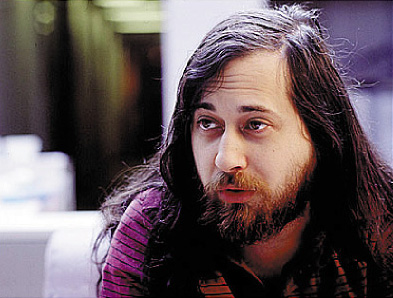
\includegraphics[width=50mm]{images/stallman.jpg}
	\caption{Richard Stallmann da giovane}
\end{figure}

\subsection{Emacs}

Una delle prime cose che Stallman fece fu la creazione di Emacs. 
Inizialmente esso era pensato come un insieme di macro per TECO, utilizzato da tutti, che era una sorta di linguaggio per scrivere e non era assolutamente real-time. 
Creò dunque una sorta di editor dentro TECO.  Guy Steele ebbe in seguito l'idea di fare un po' di ordine tra le macro (che erano diventate tantissime). 
Quest'opera fu continuata da Stallman, in modo da avere un insieme più omogeneo. Questo disordine non sarebbe dovuto replicarsi in futuro, bisognava evitare che ciascuno costruisse il proprio insieme di macro. Stallman voleva fare qualcosa di ``sociale'', voleva andare un po' oltre e impedire ulteriori disordini. Quindi si imposero delle restrizioni sulle modifiche delle macro. Questa condizione creò una sorta di comunità in cui i programmatori condividevano gli sforzi di programmazione ed evitavano la dispersione del lavoro. Questo fu il primo gruppo concreto di condivisione del software e il primo mattone della nascita della GPL. Emacs è nato in questo modo, ma poi è stato ritradotto varie volte.

\begin{figure}[htbp]
	\centering
	
\includegraphics[width=20mm]{images/emacs.png}
	\caption{Il logo di emacs}
\end{figure}

\section{La crisi del movimento hacker del MIT}

\subsection{Le prime incursioni}

Si iniziarono a vedere e prime debolezze quando il dipartimento di difesa obbligò gli hackers a programmare sui sistemi del dipartimento di \textit{computer science} del MIT in cui c'era mancanza di accesso libero all'informazione. 

Gli hacker arrivarono quindi al punto di fare una sorta di ``sciopero'' nei confronto del laboratorio, bloccarono anche l'accesso alle successive versioni di Emacs. 

Negli anni '70-'80 si creò poi una frammentazione all'interno della cultura hacker, questo perché molti hackers cominciarono a migrare, andando a lavorare per altre società.

Inoltre, iniziarono a comparire i primi programmi coperti da copyright anche all'interno del MIT.

\subsection{La Lisp machine e il collasso}

Richard Greenblatt, un programmatore del MIT, era un'autorità nel settore. 
Aveva iniziato a giocare con le LISP machine (LISP era un linguaggio ad alto livello) e aveva avuto l'idea di creare una macchina che eseguisse LISP in modo più efficiente e sicuro. 
Creò una sorta di controllo all'interno di LISP per la gestione delle risorse, aveva modificato la struttura dell'hardware in modo che LISP venisse utilizzato più velocemente. 
Questo fu un grosso passo avanti, perché programmare in LISP era molto più comodo che programmare in Assembler. 
Alla lunga riuscì ad ottenere lo stanziamento di fondi per 6 macchine. Si arrivò a produrne 32. 

Anche per gli hacker era un mondo nuovo, perché cambiava la visione classica (un solo computer disponibile), ora ogni persona aveva la propria macchina. Pensò dunque di collegare queste 32 macchine per favorire la condivisione. 
Il progetto è cresciuto a un punto tale che si trasformò in un azienda per la produzione di Lisp machine, che in un certo senso era un'estensione del MIT. 

La visione di Greenblatt era quella di un'azienda \textit{``hacker friendly''}, da mantenere senza coinvolgere investitori esterni, ma reinvestendo i soldi anticipati dai clienti. 
Russel Noftsker, che era parte del progetto, non condivideva molto l'idea e la sua visione era incompatibile con quella di Greenblatt, infatti pensava che con questa politica, l'azienda non sarebbe stata in grado di funzionare e voleva adottare una struttura aziendale più classica, dando del poter anche agli investitori esterni.

Nel 1979 si arriva al punto in cui il conflitto esplode (Greenblatt aveva dalla sua un caratteraccio, non teneva conto delle persone). Da un lato non si poteva ``far fuori Greenblatt'', ma dall'altro non c'erano molte persone che volessero continuare con la sua visione (Greenblatt voleva avere l'ultima parola), quindi in sostanza non esisteva un team. 
 
 Vennero quindi fondate due aziende, la \textbf{Lisp Machine, Inc} (LMI) di Greenblatt e la \textbf{Symbolics Inc} di Noftsker.
 
 \subsection{Lo svuotamento del MIT}
 
LMI e Symbolics attingono pesantemente dal MIT, dividendo così la comunità. 
Nel 1982 Symbolics rende le proprie modifiche al sistema operativo delle Lisp machines proprietario. A questo punto c'è un crollo della comunità, era già molto debole, erano rimasti pochi hackers ma c'era comunque un sistema complesso che andava mantenuto. 
 
Quindi a un certo punto PDP divenne obsoleto e la comunità si ritrovò di fronte a un problema, bisognava creare una nuova macchina, era necessario prendere tutto il software delle macchine correnti e riscriverlo, e gli hackers non erano abbastanza numerosi. 
 
Alla fine si decise di comprare il sistema operativo proprietario di Digital e a partire da esso si creò \textbf{Twenex}, con caratteristiche molto diverse da un sistema standard (sicurezza costruita nel sistema). 
Il gruppo \textit{wheel} era un gruppo i cui programmatori erano gli unici che potevano divenire amministratori e apportare modifiche alla macchina. In seguito ci fu la nascita di GNU.

\section{Il progetto GNU}


\subsection{In principio c'era UNIX}

Una serie di circostanze ha voluto che UNIX venisse rilasciato con licenza libera (era comunque protetto da copyright). Nasce come una risposta a \glossario{MUTIX} per creare un sistema diverso, più piccolo e con minor risorse. Fu il primo sistema scritto non direttamente in linguaggio macchina ma scritto in linguaggio C. Questo sistema ebbe subito un grosso successo anche e soprattutto in ambito universitario. 

L'AT\&T era un monopolio telefonico del governo, aveva la restrizione che non poteva vendere software e quindi si decise di distribuire gratuitamente unix. Al suo lancio esso si diffuse molto rapidamente. Una delle università che lo utilizzò fin da subito fu \textbf{Berkeley}, che aveva interesse dal punto di vista della programmazione interna di unix. Nel 1977 nacque BSD, una versione modificata di unix utilizzata dall'università. Due anni dopo la AT\&T annunciò di voler commercializzare unix. 

Nel 1983 AT\&T viene divisa e unix diventa commerciale. A questo punto c'era BSD ed era una possibile scelta. \glossario{ARPA} lo utilizzò per creare \glossario{ARPANET}, per collegare diversi computer via network, garantendo un'uniformità a livello software del sistema operativo. Il software libero ebbe quindi un impatto notevole. ARPA mise inoltre a disposizione dei fondi per migliorare BSD e facilitare il suo sviluppo. In seguito venne citata in giudizio dalla AT\&T perché si diceva volesse il codice di unix. Questo bloccò di fatto lo sviluppo di ARPANET. Se ciò non fosse successo probabilmente non sarebbe nato unix.

\subsection{La nascita di GNU}

Nel momento in cui il software è chiuso emerge la necessità di creare un movimento alternativo. Al MIT c'era una stampante, la \textit{Xerox 9700}, modificata a partire da un fax. Ma fax e stampanti hanno modi e utilizzi molto diversi. Mancava ad essa una funzionalità del driver, non comunicava al sistema operativo se la carte si era inceppata, e quindi era impossibile capirlo se non andando a verificare di persona. Richard Stallman si mise a scrivere questa funzionalità in modo che la stampante comunicasse al sistema operativo il suo stato. Però non riuscì a trovare il codice sorgente del software di essa e invano la chiese. Questo fu uno dei motivi che portarono Stallman alla creazione del progetto GNU. Ci furono diverse volte in cui Stallman si ritrovò di fronte a codice bloccato da parte del MIT. Lui si ritrovò a dover confrontarsi con questa realtà.

Nel 1983 Richard Stallman fece un appello su \texttt{net.unix-wizards}:

\begin{center}
	\textit{``Starting this Thanksgiving I am going to write a complete Unix-compatible software system called GNU (for Gnu’s Not Unix), and give it away free to everyone who can use it. Contributions of time, money, programs and equipment are greatly needed''}.
\end{center}

Le ragioni della scelta di UNIX furono:

\begin{itemize}
	\item Il monopolio della AT\&T e la chiusura di UNIX;
	\item La familiarità con il codice sorgente (e grosso utilizzo da parte delle università), c'era un grande numero di utilizzatori e di sviluppatori;
	\item La portabilità (sviluppato in C e non in Assembler), sistema che si adattasse alle macchine, su architetture molto diverse.
	
\end{itemize}

Stallman cominciò dunque a creare questo nuovo sistema operativo a partire dalla basi (compilatori, editor di testo, ...) e nel 1984 lasciò il MIT per togliergli la possibilità di rivendicare il codice scritto da lui. 

\subsection{GNU Emacs e l'origine di GPL}

La prima cosa che serviva era un programma per eseguire il codice, quindi ci fu un grosso lavoro sul compilatore. Stallman parte dal codice di Gosling e scrive GNU Emacs. L'Emacs del MIT non andava bene, serviva una nuova versione che andasse bene per le macchine piccole. Si erano nel frattempo creati tutta una serie di \textit{cloni} di Emacs, una di quelle era scritta da James Gosling e quest'ultimo concedette a Stallman il codice senza problemi, dal quale potè creare una nuova versione.

Unipress a quel punto minacciò legalmente Emacs (aveva acquistato la versione di Gosling), ma per fortuna di Stallman la versione era stata riscritta praticamente da zero, per cui non ebbe problemi e nel 1985 rilasciò ufficialmente il programma. 

Stallman decise di pensare bene a una licenza per la versione, basandosi su GNU. La licenza era basata principalmente sulla licenza implicita della comunità Emacs. È il primo grosso progetto di GNU, che sotto sotto era una GPL. A partire da esso si svilupparono tutta un'altra serie di progetti, bisognava creare dunque una licenza che fosse comune a tutti. Gilmore suggerì dunque il cambio di nome e nacque la \textbf{GNU General Public License} che venne distribuita in versione 1.0 con il rilascio di gdb.

\subsection{FSF - Free Software Foundation}

Nel 1985 Stallman fonda la Free Software Foundation, un'organizzazione no-profit allo scopo di \textit{assumere} i programmatori che sviluppavano software libero e per gestire gli aspetti legali e politici a supporto del progetto GNU, come la gestione delle licenze GPL.

Con la fondazione dell'organizzazione, Stallman rilasciò anche il manifesto del software libero (\textbf{The Free Software Definition}), che nella versione originale citava:

\begin{center}
	\textit{La parola libero nel nostro nome non si riferisce al prezzo; si riferisce alla libertà. Prima di tutto, la libertà di copiare un programma e ridistribuirlo agli altri cosicché loro possano usarlo come te. Come seconda cosa, la libertà di modificare il programma, così tu puoi controllarlo e lui non può controllarti; per questo, il codice sorgente deve essere accessibile.}
\end{center}


\subsection{L'incontro con BSD}

AT\&T cominciò a focalizzarsi sull'utilizzo di Unix a scopo commerciale e nel frattempo si sviluppò BDS, una distribuzione di Unix derivata con scopi accademici e con diversi contributi esterni. L'idea era di trasformare i loro sistemi operativi \textit{batch} con una versione di Unix.
Due studenti si erano appassionati e avevano reso una versione migliore di BSD, aggiungendo tutta una serie di cose, iniziando dapprima a effettuare modifiche esterne e poi interne. Quindi si formò una distribuzione indipendente, ma c'era la necessità della licenza AT\&T. 
Stallman convinse Bostic e i suoi a creare una versione completamente libera (all'inizio era un po' deficitaria ma col tempo si è messa in pari). A questo punto c'era un sistema operativo (e un kernel) libero.

\subsection{Anni 80-90}

Intorno alla costellazione GNU ci furono vari programmatori che iniziarono a rilasciare codice sotto licenza GPL. Bruce Perens rilascia \textit{electric fence} sotto licenza GPL, una libreria per le chiamate all'allocazione di memoria. Bruce Perens sarebbe diventato in seguito il project leader di Debian.

GPL stava dunque divenendo una licenza molto importante. Rich Marin fonda \glossario{Prime Time Freeware}, un'azienda che rilascia software solo sotto GPL. L'azienda \glossario{Cygnus} con Micheal Tiemann aveva cominciato a lavorare al progetto \glossario{gcc}, aggiungendo il supporto al C++. Il progetto era quella di contribuire (fare modifiche) al gcc e poi rivenderlo. L'idea ebbe un notevole successo. Cygnus venne fondata nel 1990 e per la fine dell'anno valeva 725000\$ in supporto e contratti.

\subsection{Espansione del progetto GNU}

Il progetto GNU si espanse in modo molto rapido e virale. Di seguito vengono riportati i maggiori rilasci dei primi anni:

\begin{itemize}
	
	\item gcc;
	\item Libc (1987);
	\item Bash (la shell), fileutils (gestione dei file), sh-utils, textutils (gestione dei testi);
	\item Ghostscript;
	\item Textinfo (formattazione della documentazione, l'html lo renderà obsoleto);
	\item Yakk, make, ...
	
\end{itemize}

\subsection{GNU Hurd}

Quello che mancava era un kernel, ed era molto complesso svilupparlo. All'inizio le macchine disponevano di un sistema unix proprietario. Vi era dunque la necessità di creare un \textbf{kernel libero}. Nel 1986 ci fu il primo tentativo di basare il kernel su TRIX, ma oltre a non funzionare sulle macchine standard richiedeva troppi cambiamenti. In seguito si sviluppò l'idea di basarsi su BSD, ma c'era poca collaborazione da parte degli sviluppatori bsd, si preferisce un approccio più ambizioso.
Svilupparono dunque un micro-kernel basato su \textbf{Mach}, ma inizialmente non era libero e dovettero aspettare che ``\textit{venisse liberato}''. Nel 1990 iniziarono dunque i lavori sul kernel, ma ci furono diverse difficoltà nello sviluppo. Poi arrivò \textbf{linux} e dunque molti sviluppatori posarono ad esso la loro attenzione. Allo stato attuale ci sono stati tutta una serie di progressi:

\begin{itemize}
	
	\item Driver linux disponibili via DDE;
	\item Supportato X, iceweasel, ...;
	\item Porting di debian.
	
\end{itemize} 

\section{Linux}

Nel 1990 nasce Linux, con un nuovo kernel a partire da Minix. All'inizio l'interesse dei GNU non era quello di creare un sistema completo, ma voleva mettere a disposizione uno strumento fin da subito (in tempi rapidi), per cui non venne progettato un kernel ma riutilizzato Minix. Il software Minix era stato sviluppato da \textit{Tanenbaum}. Da qui nacque la comunità Linux, che venne annunciata al mondo. Nel 1991 venne rilasciato Linux 0.0.2.

\subsection{MINIX}

Unix era un sistema operativo vero e proprio, ed era molto complesso. John Lions, un famoso sviluppatore Australiano, pubblica il codice sorgente commentato di UNIX in un'opera storica denominata: \textbf{Lions' Commentary on UNIX 6th Edition, with Source Code}. Ma con l'avvento della versione 7 di unix vengono imposti tutta una serie di blocchi: l'opera di Lyons viene bloccata, aumentano i costi delle licenze e vi sono delle restrizioni sull'insegnamento in classe. Molte università interruppero dunque l'insegnamento di unix; questo fu un cambiamento abbastanza stupido, perché ciò che aveva reso forte unix era la diffusione nel mondo accademico. 

Andrew S. Tanenbaum era all'epoca un insegnante di \textit{computer science} e venne molto toccato da questa decisione, in quanto aveva sempre insegnato basandosi su unix. Decise allora di creare \textbf{MINIX}, un sistema operativo abbastanza importante, minimale, per scopi didattici, pensato per essere \textbf{semplice}. Era un sistema a micro kernel, rilasciato sotto \textbf{licenza permissiva} ma non libera. Aveva inoltre scritto un libro che documentava e spiegava MINIX. Ma questo sistema operativo aveva una grossa limitazione: \textbf{mancava un emulatore di terminale}.

\subsection{Linus Torvalds e la nascita di Linux}

Linus Torvalds è stato uno dei primi utilizzatori di MINIX. Nasce ad Helsinki nel 1969. Nel 1990 frequenta l'Università di Helsinki, comincia a studiare Tanenbaum e comincia a fare le prime modifiche per provare a creare un emulatore di terminale. Nel 1991 Lars Wirzenius (un amico di Torvalds) lo porta alla conferenza di Stallman, nella quale ebbe una prima esposizione al progetto GNU. Il 5 Gennaio 1991 Torvalds:

\begin{itemize}
	
	\item Compra un PC (un 80386);
	\item Ci installa MINIX;
	\item Inizia a scriverci un emulatore di terminale (scritto in C e in assembly).
	
\end{itemize}

\begin{figure}[htbp]
	\centering
	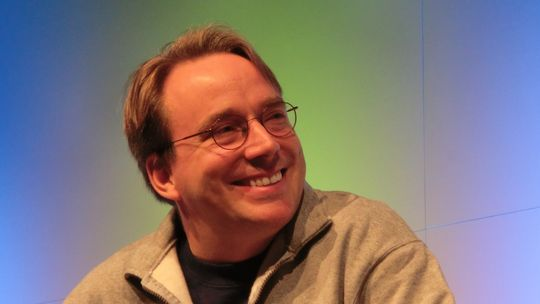
\includegraphics[width=50mm]{images/linus-torvalds.jpg}
	\caption{Linus Torvalds}
\end{figure}

La prima versione di \textbf{Linux} è la A e la B, fatta solamente da due finestre. Da emulatore di terminale com'era pensato in origine Linux d lì il è stato espanso fino a crearci un vero e proprio sistema operativo \textbf{Linux 0.0.1} con un kernel funzionante.

Già nel 1992 il sistema era diventato molto importante. Torvalds decide dunque di rendere il sistema \textbf{indipendente} da MINIX (ci fu anche una disputa con Tanenbaum). Cambiò dunque la licenza adottando la GPL, che considerava buona per il suo sistema operativo, a prescindere dal software GNU stesso. Nascono inoltre già le prime distribuzioni basate su linux, come ad esempio SUSE, MCC o la prima distribuzione commerciale: LGX. Queste distribuzioni rendevano decisamente più facile l'utilizzo di Linux (di per sè molto complesso).

Nel 1994 viene rilasciato \textbf{Linux 1.0} e fu lo stesso Torvalds a presentarlo in una conferenza tenutasi ad Helsinki. Già allora era un sistema utilizzabile.

Ancora nel 1993 erano nate le prime versioni commerciali: Bolzern, Flagship e \textbf{Linux Pro}. Nel 1994 nasce inoltre \textbf{RedHat}, creato da Marc Ewing, e diventa ben presto la più diffusa distribuzione Linux.

Nel 1996 fu scelto come logo ufficiale di Linux un pinguino disegnato da Larry Ewing, chiamato \textbf{Tux}, come abbreviazione di \textbf{T}orvalds \textbf{U}nix.

Sempre nel 1996 esce \textbf{Linux 2.0} con supporto a microprocessore. Con la versione 3.0, uscita nel 2011, le modifiche sono state molto più incrementali. Nel corso degli anni con la 2.0 il grado di utenza era ancora molto piccolo.

\begin{table}[htp]
	\centering
	\begin{tabular}[c]{l | l | l}
		\hline
		& 1992 & 2012 \\
		\hline
		Sviluppatori Linux & 100 & 1000 \\
		\hline
		Linee di codice Linux & 250.000 & 14.000.000 \\
		\hline
	\end{tabular}
	\caption{Sviluppo di Linux negli anni}
\end{table}

Una volta c'erano molti sviluppatori \textit{volontari}, ad oggi il supporto è dato da grosse aziende che possono investire tempo e denaro su Linux.

\subsection{Debian}

C'era un forte legame tra il mondo degli hackers e il mondo del software libero. Si venne a creare una \textbf{nuova generazione di sviluppatori}. Volevano provare a costruire una distribuzione che fosse fortemente legata a certi principi, che mettesse insieme varie cose, che facesse da collante. A quel punto nacque \textbf{Debian}. Linux da un lato stava procedendo e crescendo velocemente ed aveva molte caratteristiche interessanti, ma dall'altro c'era una lontananza dai principi del software libero e dalla GNU. Questo era percepito come un problema da parte di una fetta della comunità. Ad altri invece la cosa andava più che bene, dunque si venne a creare una \textbf{divergenza}. 

Il progetto Debian venne fondato da Ian Murdock nel 1993, con l'intento di fare una distribuzione di Linux \textbf{completamente libera}. Entrò a far parte del progetto GNU nel 1994-1995. Nel 1994 venne redatto il \textbf{manifesto debian}, nel quale si riassumeva il significato e la filosofia di debian. La prima versione stabile (Debian 1.1 ``Buzz'') venne rilasciata nel 1996. Il project leader della Debian divenne Bruce Perens

La caratteristica principale di Debian è che pone l'attenzione in modo quasi maniacale alla qualità del software (a volte perdendo anche molto tempo) e al fatto che il software sia libero (solo software DFSG. Si basa su una \textbf{forte comunità} che gestisce (tramite votazioni) tutte le decisioni sullo sviluppo; chiunque può proporre cambiamenti e ognuno è responsabile delle proprie azioni (attenzione alla sicurezza). Un altro cardine su cui puntano gli sviluppatori Debian è una strenua \textbf{disponibilità} del software.

Debian è caratterizzato da un suddivisione (politica) in più parti del repository. Le uniche componenti che sono della Debian sono quelle libere e quelle che dipendono da software libero. Il software che è all'interno della Debian entra nell'archivio principale, \textbf{FREE}. Poi all'interno ci sono altre componenti ospitate nel server della Debian ma che non sono della Debian, \textbf{NON-FREE} che non aderisce alle \textit{DFSG}, \textbf{CONTRIB} (che è libero ma dipende da componenti non libere).

C'è una versione di Debian \textbf{stabile} (software un po' vecchio però), quella che ha superato tutti i bugfix, una versione \textbf{non stabile} e una versione \textbf{testing}. Nella versione non stabile ``\textit{può esplodere tutto da un momento all'altro}'', viene aggiornata ogni giorno. La testing entra nel pacchetto solamente se nell'ultimo mese non sono stati segnalati bug importanti.

Da un lato Debian ha molto software e dall'altro non avendo interessi commerciali, non ha interessi nel penalizzare la concorrenza. È gestita essenzialmente da volontari.

\subsection{Un po' di ordine}

\begin{itemize}
	\item Stallman con il progetto GNU voleva creare un nuovo sistema operativo, alternativo ad UNIX.
	\item Vengono sviluppati vari programmi, ma manca ancora un kernel. GNU Hurd doveva essere il kernel, ma lo sviluppo è stato lento.
	\item Linus crea Linux e viene utilizzato come kernel per GNU.
	\item Con il tempo Linux cambia ed inizia ad utilizzare anche del software proprietario. Diventano quindi distinti il progetto GNU e Linux. GNU/Linux è una distribuzione che utilizza una versione di Linux completamente libera. Al giorno d'oggi esistono anche GNU/Hurd e GNU/kFreeBSD.
	\item Linux è pubblicato sotto licenza GPLv2.
\end{itemize}

	\chapter{Il movimento Open Source}

\section{La storia del movimento Open Source}

\subsection{La cattedrale e il bazaar}

Un altro personaggio molto importante nel mondo del software libero è Eric Steven Raymond, informatico e programmatore statunitense di grande esperienza, che nel 1997 pubblica ``\textbf{La cattedrale e il bazaar}'', un saggio sullo sviluppo del software. Esso era essenzialmente destinato ad affrontare il problema del perché Linux, con il suo kernel, funzionasse così bene. Non era scontato che Linux funzionasse, anzi all'inizio, secondo la sua opinione, era destinato a ``scoppiare''. Il problema è che ognuno tendeva a pensare con la propria testa; eppure la cosa non succedeva. Quindi iniziò ad analizzare il fenomeno. 

Una delle prime cose che ha fatto è stato quello di iniziare un progetto, chiamato \textbf{popclient}, per l'invio e la ricezione della posta. Comincia dunque ad utilizzare tutta una serie di principi per la gestione di questo progetto per vedere se riusciva a ricreare il successo che aveva visto con Linux, un progetto che funzionasse bene e avesse una solida base di sviluppatori. Uno dei principi che aveva adottato era di trattare gli utenti come una sorta di \textbf{co-sviluppatori}, come se il programma fosse stato fatto insieme a loro. La comunità popclient divenne dunque molto attiva. 

Il secondo principio su cui basò il proprio lavoro fu: ``Distribuisci presto, distribuisci spesso e presta ascolto agli utenti'', in questo modo si favorisce la risoluzione di bachi in tempi brevi. Molti utenti si facevano avanti e miglioravano il software, sentendosi parte attiva del progetto. L'idea che secondo Raymond aveva fatto il successo di Linux era trasformare il software da uno sviluppo di una persona che ``dona agli altri'' a uno sviluppo ``social'', attorno al quale ruotava una comunità. Spesso la varietà delle persone porta ad una varietà di modi per risolvere il problema, vi sono approcci diversi, e la combinazione dei contributi può significare grossi miglioramenti.

L'articolo di Raymond ebbe una grossissima fortuna, l'impatto all'interno della comunità fu molto sentito, e l'effetto di questo fu che l'attenzione andò oltre la semplice comunità degli appassionati. Una delle conseguenze di questo successo fu che nel 1998 Netscape annunciò di voler rilasciare il codice sorgente del proprio browser, e disse che per decidere questo si era basato anche sull'articolo di Raymond. Una volta Netscape era dominante, prima dell'arrivo del colosso Microsoft con Internet Explorer. Il browser di casa Microsoft è sicuramente disprezzato al giorno d'oggi, ma in realtà per gli standard di allora era molto buono e la Microsoft era riuscita, partendo da zero, a recuperare terreno in tempi notevoli su Netscape. A Netscape non interessava moltissimo del suo navigatore, non poteva infatti guadagnarci (era gratis), ma focalizzava la sua attenzione sul mondo Server. Temeva però che se Internet Explorer fosse divenuto dominante a quel punto i propri server sarebbero stati ``scartati'' in favore di quelli di Microsft. Avrebbe perso una grossa fetta di mercato e buona parte del loro reddito. Ebbero dunque l'idea di rilasciare il codice sorgente di Netscape sotto una licenza libera. In questa decisione aveva avuto un ruolo importante Raymond, che divenne dunque una celebrità.

C'era però il rischio che il termine ``software libero'' si svalutasse o non acquisisse la giusta importanza. Ci fu dunque una riunione su come sfruttare al massimo l'annuncio di Netscape: nasce il termine ``\textbf{open source}''. L'idea era che il software libero garantiva software di maggiore qualità ai fini di offrire una piattaforma stabile, con una buona comunità e aperta. Nel 1998 nasce dunque la \textbf{Open Source Initiative}, fondata da Raymodn e Perens, che aveva come scopo quello di diffondere il mondo open source. In questo movimento entrarono a far parte tutti gli sviluppatori più importante, come RedHat. 

\subsection{Riassumendo}

Nel 1997 nasce il movimento open-source, Raymond pubblica ``\textit{The Cathedral and the Bazaar}'' (presentato alla O'Reilly Perl Conference). Raymond si mise ad analizzare la diffusione di Linux. Si crea un modello di sviluppo che invece di essere a cattedrale è a bazaar (come un mercato, in cui ci sono tante persone che contribuiscono tutte in modo diverso). Con questa nuova ottica si riesce dunque a produrre software in modo migliore.

Nel 1998 Netscape rilasciò il sorgente del proprio browser. Netscape all'epoca controllava il mercato dei browser ma era in crisi con l'incursione del colosso Microsoft e l'avvento di Internet Explorer. Temevano che la Microsoft sarebbe divenuta dominante e quindi rilasciarono il codice sorgente (primo grande rilascio della storia), il che costrinse inoltre loro ad un'ingente pulizia del codice (codice scritto male e con tanta spazzatura). Questo fu un passo epocale, infatti \textit{Firefox} nacque da questo. All'interno della comunità ci fu subito la percezione che questo rilascio fosse molto particolare e fosse qualcosa da sfruttare. L'interesse era creare un sistema funzionante e che si facesse rispettare. Nasce dunque il concetto di open-source e la OSI. Ci si rese conto che la produzione di software libero coincide con la produzione di software migliore. I grossi leader entrarono in questo movimento. Nel 2000 Sun richiese il codice sorgente di StarOffice. Mancava infatti un software di produttività che fosse all'altezza di ad esempio \textit{Microsoft Office}.

Per evitare che il termine venisse diluito e svalutato ci fu la necessità di renderlo un \textbf{marchio}, in modo che un software per essere considerato libero dovesse rispettare questo marchio ed essere approvato dalla OSI. 

\subsection{Open Source Definition}

Ci fu quindi la creazione di una serie di \textbf{linee guida} chiare per considerare un software come open-source. L'idea era quella di riutilizzare le Linee guide della Debian, le DFSG, in vigore dal 1997 rendendole più adatte in senso generale. Queste linee guida sono state sviluppate dall'interazione di decine di sviluppatori e sono state pensate in modo da non lasciare fuori tanto software libero importante già esistente.

\begin{itemize}
	
	\item Libera redistribuzione;
	\item Inclusione del codice sorgente;
	\item La licenza deve permettere modifiche e lavori derivati e deve permettere la loro distribuzione con i medesimi termini della licenza del software originale;
	\item Integrità del codice sorgente dall'autore, modifiche che esplicitino ``chi ha fatto cosa'', in modo che chiunque sia responsabile di ciò che scrive;
	\item Nessuna discriminazione di persone o gruppi;
	\item Nessuna discriminazione per i campi di impiego;
	\item La licenza dev'essere distribuita, per fare chiarezza;
	\item La licenza non può essere specifica per Debian;
	\item La licenza non deve contaminare altro software, non si possono imporre condizioni su software già esistente. La licenza dev'essere indipendente.
	
\end{itemize}


\section{La filosofia open source}

Questi principi, che sono delle vere e proprie clausole, sono tutti pragmatici: quello che conta è costruire software che sia affidabile e veloce in modo analogo a Linux:

\begin{itemize}

\item \textbf{Licenze libere e permissive}; quando una licenza è chiusa si tratta gli utenti non come co-sviluppatori ma come ``utenti di serie B''. È come dire: ``\textit{Vabbè, se proprio vuoi fammi il bug reporting...}'' oppure ``\textit{Tu sei talmente inutile per me che nemmeno ti aiuto ad aiutarti...}''. È un principio che in casa Microsoft va bene, perché l'obiettivo non è costruire una comunità. Nel caso del mondo open-source fare così è come ``darsi la mazza sui piedi'';
\item \textbf{Costruzione di una comunità attorno al software}; il software non è più una cosa che viene \textit{usata}, ma un modo di vivere, una cosa in cui le persone sono coinvolte. Con la crescita e lo sviluppo di una comunità attorno al software non solo i bachi vengono risolti più rapidamente, ma si hanno anche nuovi apporti mentali e contributi da parte delle persone;
\item \textbf{Trasparenza del processo di sviluppo}; la gente deve vedere quello che sta succedendo, perché una volta che lo vede magari contribuisce. Questo tipo di comunicazione è fondamentale;
\item \textbf{Codice sorgente liberamente disponibile}; altrimenti non possono esserci trasparenza e contributi da parte della comunità;
\item \textbf{Codice sorgente liberamente modificabile};
\item \textbf{Libera redistribuzione}, anche ad uso commerciale;

\end{itemize}

\section{Open Source Definition}

L'Open Source Definition è nata perché quando si è sviluppato il movimento OSI (\textit{Open Source Initiative}) ci si è reso conto che c'era il rischio, soprattutto nel momento in cui il movimento open source avesse avuto un forte impatto, che nella barca sarebbero saltati molti altri partecipanti ma non tutti avrebbero collaborato rispettando appieno le regole. Quindi era vitale decidere delle norme, delle linee guida da rispettare per scrivere del software open source. Esse erano pensate per escludere il minor numero di programmi già esistenti (esempio TEX, Perl, ...). Questo progetto ambiva a dare una caratterizzazione del software libero.

\subsection{Libera redistribuzione}

\begin{center}

\textit{La licenza non può limitare alcuno dal vendere o donare il software che ne è oggetto, come componente di una distribuzione aggregata, contenente programmi di varia origine. La licenza non può richiedere diritti o altri pagamenti a fronte di tali vendite.}

\end{center}

\textbf{Motivazione}: Imponendo la libera redistribuzione, si elimina la tentazione di rinunciare a importanti guadagni a lungo termine in cambio di un guadagno materiale a breve termine, ottenuto con il controllo delle vendite. Se non vi fosse questa imposizione, i collaboratori esterni sarebbero tentati di abbandonare il progetto, invece che di farlo crescere.

\subsection{Codice sorgente}

\begin{center}

\textit{Il programma deve includere il codice sorgente e ne deve essere permessa la distribuzione sia come codice sorgente che in forma compilata. Il codice sorgente deve essere il formato preferito per effettuare modifiche al codice.}

\end{center}

\textbf{Motivazione}: si richiede l'accesso al codice sorgente poichè non si può far evolvere un programma senza poterlo modificare. Il nostro obiettivo è rendere facile l'evoluzione del software, pertanto richiediamo che ne sia resa facile la modifica.

\subsection{Prodotti derivati}

\begin{center}

\textit{La licenza deve permettere modifiche e prodotti derivati, e deve permetterne la redistribuzione sotto le stesse condizioni della licenza del software originale.}

\end{center}

\textbf{Motivazione}: la sola possibilità di leggere il codice sorgente non è sufficiente a permettere la revisione indipendente del software da parte di terzi e una rapida selezione evolutiva. Per garantire una rapida evoluzione, deve essere possibile sperimentare modifiche al software e redistribuirle.

\subsection{Discriminazione contro persone o gruppi}

\begin{center}

\textit{La licenza non deve discriminare alcuna persona o gruppo di persone.}

\end{center}

\textbf{Motivazione}: per ottenere il massimo beneficio dal processo, il massimo numero di persone e gruppi deve avere eguale possibilità di contribuire allo sviluppo del software. Pertanto viene proibita l'esclusione arbitraria dal processo di persone o gruppi.

\subsection{Integrità del codice sorgente originale}

\begin{center}

\textit{La licenza può impedire la distribuzione del codice sorgente in forma modificata, a patto che venga consentita la distribuzione dell'originale accompagnato da ``patch'', ovvero file che permettono di applicare modifiche al codice sorgente in fase di compilazione.}

\end{center}

\textbf{Motivazione}: incoraggiare il miglioramento è bene, ma gli utenti hanno diritto di sapere chi è responsabile del software che stanno usando. Gli autori e i tecnici hanno diritto reciproco di sapere cosa è loro chiesto di supportare e di proteggersi la reputazione.

\subsection{Discriminazione per campo d'applicazione}

\begin{center}

\textit{La licenza non deve impedire di far uso del programma in un ambito specifico.}

\end{center}

\textbf{Motivazione}: L'intenzione principale di questa clausola è di proibire trappole nelle licenze che impediscano al software open source di essere usato commercialmente. Vogliamo che le aziende si uniscano alla nostra comunità, non che se ne sentano escluse.

\subsection{Distribuzione della licenza}

\begin{center}

\textit{I diritti allegati a un programma devono essere applicabili a tutti coloro a cui il programma è redistribuito, senza che sia necessaria l'emissione di ulteriori licenze.}

\end{center}

\textbf{Motivazione}: questa clausola intende proibire la chiusura del software per mezzi indiretti, come un obbligo di sottoscrizione di accordi di non diffusione.

\subsection{Specificità ad un prodotto}

\begin{center}

\textit{I diritti allegati al programma non devono dipendere dall'essere il programma parte di una particolare distribuzione del software.}

\end{center}

\textbf{Motivazione}: questa clausola impedisce un'ulteriore classe di licenze-trappola

\subsection{Vincoli su altro software}

\begin{center}

\textit{La licenza non deve porre restrizioni su altro software distribuito insieme al software licenziato.}

\end{center}

\textbf{Motivazione}: i distributori di software open source hanno il diritto di fare le loro scelte riguardo al software che intendono distribuire.

\subsection{Neutralità rispetto alle tecnologie}

\begin{center}

\textit{La licenza non deve contenere clausole che dipendano o si basano su particolari tecnologie o tipi di interfacce.}

\end{center}

\textit{Nota}: no al mouse click obbligatorio.

\section{Confronto con il Software Libero}

Il software Open Source ha dei criteri leggermente più deboli di quelli previsti per il software libero. Entrambi però sono accomunati dalla necessità che il codice sorgente sia disponibile e la maggior parte delle volte, il software open source è anche libero e viceversa.
Ci sono però delle licenze Open Source che non sono ritenute libere.

In ogni caso perché il software possa essere definito Open Source deve rispettare la OSD, mentre per essere libero deve rispettare le 4 libertà fondamentali del manifesto del software libero delle FSF e non può essere che uno dei due manifesti non venga rispettato, perché ad esempio esistono delle licenze Open che non prevedono il copyleft.

Tra i due movimenti c'è una differenza sostanziale riguardo le motivazioni. Il software libero punta di più sulla questione morale mentre il software Open da maggior peso ai vantaggi pratici.

Sempre nel lato pratico, l'Open Source viene preferito dalle aziende perché il termine ``\textit{free software}'' viene spesso associato al software gratuito.


	\chapter{Licenze software}

\section{Capisaldi}

Il diritto d'autore arriva fino a 70 anni dopo la morte. Al giorno d'oggi in realtà la grande maggioranza dei libri hanno un utilità che dura pochi anni da quando sono stati prodotti, a meno che non sia un grande classico o un best-seller. La protezione è espressa sotto forma percepibile, dev'essere qualcosa che uno ``ha creato''. Inoltre non c'è nessuna registrazione necessaria per avere il diritto d'autore. Un discorso a parte è il \textbf{work for hire}, ovvero quando qualcuno produce un'opera lavorando per qualcun altro. Quando si lavora come dipendenti, a meno di clausole particolari, tutto ciò che si produce è proprietà del datore di lavoro, viene ceduta la proprietà intellettuale del proprio lavoro all'azienda.  

Una cosa che vedremo molto spesso sono le \textbf{garanzie}, perché ogni copyright, soprattutto quelli open source, hanno una clausola che il più possibile cerca di raggiungere una certa forma di garanzia, in modo da non dover andare incontro a problematiche. Ci sono due tipi di garanzie:

\begin{itemize}

\item \textbf{Garanzie esplicite}, sono quelle che io do esplicitamente per cercare di rendere più appetibile la mia vendita; 

\item \textbf{Garanzie implicite}, che di fatto sono ``forzate'' dalla legge; esempio garanzie di commerciabilità sui prodotti acquistati, o quelle di idoneità a un certo scopo.

\end{itemize}

\section{X License (MIT license)}

È la licenza più basilare, licenza originale di X Windows. Essenzialmente permette di \textit{fare tutto}, libertà di modifica, di copia, di ridistribuzione del software. Il codice sorgente può essere redistribuito liberamente, senza restrizioni sul formato (ad esempio si può scegliere di redistribuirlo solo in forma binaria). Quello che è necessario è \textbf{mantenere la licenza originale}, in modo che la persona possa vedere la licenza con la quale è stato prodotto quel software. Ci sono naturalmente delle clausole di salvaguardia. 	

\begin{lstlisting}[caption=Licenza MIT]
Copyright (c) <year> <copyright holders>

Permission is hereby granted, free of charge, to any person
obtaining a copy of this software and associated documentation
files (the ``Software''), to deal in the Software without
restriction, including without limitation the rights to use,
copy, modify, merge, publish, distribute, sublicense, and/or sell
copies of the Software, and to permit persons to whom the
Software is furnished to do so, subject to the following
conditions:

The above copyright notice and this permission notice shall be
included in all copies or substantial portions of the Software.

THE SOFTWARE IS PROVIDED ``AS IS'', WITHOUT WARRANTY OF ANY KIND,
EXPRESS OR IMPLIED, INCLUDING BUT NOT LIMITED TO THE WARRANTIES
OF MERCHANTABILITY, FITNESS FOR A PARTICULAR PURPOSE AND
NONINFRINGEMENT. IN NO EVENT SHALL THE AUTHORS OR COPYRIGHT
HOLDERS BE LIABLE FOR ANY CLAIM, DAMAGES OR OTHER LIABILITY,
WHETHER IN AN ACTION OF CONTRACT, TORT OR OTHERWISE, ARISING
FROM, OUT OF OR IN CONNECTION WITH THE SOFTWARE OR THE USE OR
OTHER DEALINGS IN THE SOFTWARE.

\end{lstlisting}

\noindent L'obiettivo è quello di \textbf{proteggere} chi ha scritto software sotto questa licenza, ecco perché ci sono tutta una serie di garanzie, in questo modo si evitano problemi futuri dovuti alla redistribuzione. Qualunque tipo di garanzia possibile è \textbf{coperta}, anche se non sempre queste clausole sono valide, ad esempio potrebbero non essere validi in alcuni paesi. Ad ogni modo, nonostante queste garanzie, è una licenza che risulta comunque molto permissiva. 

\section{Licenze BSD}

Sono leggermente più restrittive rispetto alla licenza MIT. In realtà ce ne sono diverse:

\begin{itemize}

\item BDS a 4 clausole;
\item BSD a 3 clausole;
\item BSD a 2 clausole.

\end{itemize}

\noindent Storicamente si sono sviluppate in ordine decrescente, man mano hanno tolto una clausola perché sostanzialmente creava dei problemi. La licenza BSD a quattro clausole si è dimostrata infatti inutilizzabile nella pratica, perché diveniva ingestibile tenere conto di tutti gli autori del software. 

\subsection{BDS a due clausole}

È la licenza di \textbf{NetBSD} e di fatto corrisponde alla MIT license, con l'aggiunta dell'obbligo di inserire la documentazione anche nella redistribuzione.

\begin{lstlisting}[caption=BSD a due clausole (NetBDS)]
Copyright (c) <anno>, <proprietario>
All rights reserved.

La ridistribuzione e l'uso di formule binarie, con o senza modifiche, sono permesse
purché siano rispettate le seguenti condizioni:

1. Le ridistribuzioni di codice originale devono conservare la nota di copyright 
    sopra riportato, questa lista di condizioni e il seguente disconoscimento.

2. Le ridistribuzioni in formule binarie devono riprodurre la nota di copyright 
    sopra riportata, questa lista di condizioni e il seguente disconoscimento nella
   documentazione e/o altri materiali forniti con la distribuzione.

Questo software è fornito dal <possessore di copyright> "così com'è" e qualsiasi
garanzia espressa o implicita, che includa, ma che non sia limitata a, garanzie 
implicite di commerciabilità e idoneità a scopo particolare, viene disconosciuta. 
In nessun caso il possessore di copyright sarà ritenuto responsabile per qualsiasi 
danno diretto, indiretto, connesso, particolare, esemplare o conseguente 
(includente, ma non limitato a, approvvigionamenti di beni o servizi alternativi;
perdita di utilità, dati o profitti; interruzione di affari) comunque causati e su 
qualsiasi ipotesi di responsabilità, come da contratto, responsabilità oggettiva, o 
torto (compresa negligenza o altro) derivante in qualsiasi modo dall'utilizzo di 
questo software anche se al corrente della possibilità di tale danno.

Le volontà e le finalità contenute nel software e nella documentazione sono quelle
degli autori e non vanno interpretate come rappresentazione delle politiche ufficiali,
sia espresse che implicite, del progetto FreeBSD.
\end{lstlisting}

\noindent Essenzialmente si può pensarla come una licenza BSD in cui nella distribuzione in forma binaria bisogna mantenere tutta la documentazione e la licenza. 

\subsection{BSD a tre clausole}

La BSD a tre clausole ha un'impostazione un po' più innovatoria. Si tratta comunque di una licenza molto ``generosa'', non sono per nulla invasive. Comprende le due clausole precedenti più la seguente:

 \begin{lstlisting}[caption=BSD a tre clausole]
3. Né il nome della <organizzazione>, né i nomi dei suoi collaboratori possono 
   essere utilizzati per avallare o promuovere prodotti derivati da questo software
   senza uno specifico permesso scritto.
\end{lstlisting} 

\noindent In pratica permette di ``fare quello che si vuole'' però non è possibile farsi pubblicità usando il nome del copyright holder a meno che non si abbia un permesso. Ad esempio non si può dire ``il mio software è più sicuro perché è sotto licenza BSD''. È una delle licenze più comuni nei sistemi BSD, non crea nessun problema, ed è approvata dalla OSI.

\subsection{BSD a quattro clausole}

Ma la licenza originale di BSD unix aveva un'altra clausola che era molto più invasiva. Aveva le stesse clausole già viste, in più:

\begin{lstlisting}[caption=BSD a quattro clausole] 
4. Ogni materiale pubblicitario che riporti caratteristiche o uso di questo software
   deve mostrare la seguente attestazione:
   Questo prodotto include software sviluppati dalla <organizzazione>.
\end{lstlisting}

\noindent Chiaramente questo valeva per tutti gli autori e le entità che avevano donato il codice, quindi diventava un po' problematico riportarli tutti, tanto è vero che non è stata approvata dalla OSI. Un problema più serio è che non è compatibile con la GPL perché questa clausola aggiuntiva non è prevista dalla GPL. Quindi se si voleva cambiare la licenza del prodotto a GPL si riscontravano grossi problemi in quanto si dovrebbe togliere questa clausola. Da un punto di vista pratico era inoltre molto problematico dover tener traccia di tutti gli autori (gli indirizzi email per esempio possono cambiare nel tempo).

\subsection{Considerazioni OSI/FSF}

La versione originale della licenza BSD, quella con 4 clausole, \textbf{non} viene considerata dalla OSI come licenza Open Source anche se la FSF la considera come una licenza libera ma non compatibile con la GPL.

Le versioni con 2 e 3 clausole sono considerate dalla OSI come licenze Open Source e sono anche compatibili con la GPL.

\section{Apache License}

La Licenza Apache è una licenza di software libero non copyleft scritta dalla \textbf{Apache Software Foundation} (ASF) che obbliga gli utenti a preservare l'informativa di diritto d'autore e d'esclusione di responsabilità nelle versioni modificate.

Come ogni licenza di software libero, la licenza Apache consente agli utenti di usare il software per ogni scopo, di distribuirlo, modificarlo e di distribuire versioni modificate del software.

La licenza Apache \textbf{non richiede che versioni modificate del software siano distribuite secondo i termini della stessa licenza o come software libero}, richiede solo che si includa un'informativa del fatto che si è utilizzato software licenziato secondo i termini della Licenza Apache.

Quindi, a differenza di quanto accade con le licenze copyleft, gli utenti di versioni modificate del software licenziato secondo i termini della Licenza Apache non godono necessariamente delle suddette libertà o, considerando la situazione dal punto di vista del licenziatario, esso ha la libertà di utilizzare il software in ogni modo, anche in prodotti proprietari, a danno degli utilizzatori (vedi l'articolo 4).

\subsection{Versioni}

Ci sono state tutta una serie di versioni di questa licenza, che è cambiata dalla 1.0 fino alla 2.0. La \textbf{1.0} era una BSD a quattro clausole più una clausola di rinomina, che essenzialmente diceva che se si prendeva un prodotto che utilizzava del codice di Apache era necessario chiamare il prodotto in modo diverso da Apache. Questa clausola voleva ottenere l'effetto di evitare che il codice sorgente di Apache fosse la base di una miriade di web server diversi che utilizzavano quel codice lì, volevano evitare una frammentazione eccessiva, perché sarebbe stato un danno per la comunità. 

Nella versione \textbf{1.1} hanno modificato queste cose, hanno tolto la quarta clausola di BSD, la clausola di rinomina è rimasta, e hanno aggiunto una clausola pubblicitaria sulla documentazione; in pratica era necessario pubblicizzare nella documentazione il fatto che il codice si basasse sul prodotto Apache. 

\begin{lstlisting}[caption=licenza Apache 1.1]
 ====================================================================
 The Apache Software License, Version 1.1

 Copyright (c) 2000 The Apache Software Foundation.  All rights
 reserved.

 Redistribution and use in source and binary forms, with or without
 modification, are permitted provided that the following conditions
 are met:

 1. Redistributions of source code must retain the above copyright
    notice, this list of conditions and the following disclaimer.

 2. Redistributions in binary form must reproduce the above copyright
    notice, this list of conditions and the following disclaimer in
    the documentation and/or other materials provided with the
    distribution.

 3. The end-user documentation included with the redistribution,
    if any, must include the following acknowledgment:
       "This product includes software developed by the
        Apache Software Foundation (http://www.apache.org/)."
    Alternately, this acknowledgment may appear in the software itself,
    if and wherever such third-party acknowledgments normally appear.

 4. The names "Apache" and "Apache Software Foundation" must
    not be used to endorse or promote products derived from this
    software without prior written permission. For written
    permission, please contact apache@apache.org.

 5. Products derived from this software may not be called "Apache",
    nor may "Apache" appear in their name, without prior written
    permission of the Apache Software Foundation.

 THIS SOFTWARE IS PROVIDED ``AS IS'' AND ANY EXPRESSED OR IMPLIED
 WARRANTIES, INCLUDING, BUT NOT LIMITED TO, THE IMPLIED WARRANTIES
 OF MERCHANTABILITY AND FITNESS FOR A PARTICULAR PURPOSE ARE
 DISCLAIMED.  IN NO EVENT SHALL THE APACHE SOFTWARE FOUNDATION OR
 ITS CONTRIBUTORS BE LIABLE FOR ANY DIRECT, INDIRECT, INCIDENTAL,
 SPECIAL, EXEMPLARY, OR CONSEQUENTIAL DAMAGES (INCLUDING, BUT NOT
 LIMITED TO, PROCUREMENT OF SUBSTITUTE GOODS OR SERVICES; LOSS OF
 USE, DATA, OR PROFITS; OR BUSINESS INTERRUPTION) HOWEVER CAUSED AND
 ON ANY THEORY OF LIABILITY, WHETHER IN CONTRACT, STRICT LIABILITY,
 OR TORT (INCLUDING NEGLIGENCE OR OTHERWISE) ARISING IN ANY WAY OUT
 OF THE USE OF THIS SOFTWARE, EVEN IF ADVISED OF THE POSSIBILITY OF
 SUCH DAMAGE.
 ====================================================================

 This software consists of voluntary contributions made by many
 individuals on behalf of the Apache Software Foundation.  For more
 information on the Apache Software Foundation, please see
 <http://www.apache.org/>.

 Portions of this software are based upon public domain software
 originally written at the National Center for Supercomputing Applications,
 University of Illinois, Urbana-Champaign.

\end{lstlisting}

\noindent L'Apache 1.1 non è durata molto, in quanto è subentrata poi l'Apache \textbf{2.0}, che cambia completamente. Mentre dalla 1.0 alla 1.1 hanno cambiato un po' di clausole, con la 2.0 ci sono cambiamenti molto grandi, ed è la prima licenza che analizziamo che affronta il \textbf{problema dei brevetti}. L'idea fondamentale dell'Apache 2.0 è di affrontare il problema dei brevetti. La questione è che le licenze software libere erano state formate in un momento in cui la proprietà intellettuale significava copyright. Questo non era più vero, piano piano era divenuta sempre più pressante il \textbf{problema dei brevetti}. Non si è infatti obbligati a fornire delle licenze per i brevetti, è a discrezione del proprietario. Anche dentro Apache si sono posti dunque il problema di evitare che qualcuno potesse crearsi il proprio web server che aveva tutte le funzionalità di Apache, aggiungergi delle proprie funzionalità (algoritmi) delle quale possedeva i brevetti e reimmettere nel mercato questa nuova versione. Si impose dunque una clausola sui brevetti, in cui quando una persona contribuiva ad Apache forniva anche i propri brevetti. Era necessario di distinguere il concetto di \textbf{modifica} da quello di \textbf{contribuzione}. Si pensa al modello in cui c'è uno \textbf{sviluppo centralizzato}.

I due files che devono essere inclusi nella directory principale dei prodotti software distribuiti sono:

\begin{itemize}

\item \textbf{LICENSE} - una copia della licenza.
\item \textbf{NOTICE} - un'``informativa'' testuale che elenca i nomi delle librerie licenziate che sono utilizzate, con i nomi degli sviluppatori. Nel codice redistribuito si deve preservare in ogni file licenziato qualsiasi informativa di diritto d'autore e di brevetti presente ed in ogni file modificato si deve aggiungere un'informativa specificando che il file è stato modificato.

\end{itemize}

\begin{lstlisting}[caption=licenza Apache 2.0]
Copyright [yyyy] [name of copyright owner]

Licensed under the Apache License, Version 2.0 (the "License");
you may not use this file except in compliance with the License.
You may obtain a copy of the License at

    http://www.apache.org/licenses/LICENSE-2.0

Unless required by applicable law or agreed to in writing, software
distributed under the License is distributed on an "AS IS" BASIS,
WITHOUT WARRANTIES OR CONDITIONS OF ANY KIND, either express or implied.
See the License for the specific language governing permissions and
limitations under the License.

\end{lstlisting}

\subsection{Considerazioni OSI/FSF}

Tutte le versioni delle licenze Apache sono considerate libere dalla FSF e approvate anche dall'OSI. Tuttavia solo la Apache 2.0 è ritenuta compatibile con la GPLv3.


\section{Accademic Free License}

L'Accademic Free License è una licenza permissiva libera simile alla licenza BSD con 3 clausole, ma che permette di rendere il software proprietario.

Vengono però aggiunte alcune clausole per risolvere alcuni problemi:

\begin{itemize}
	\item Viene reso chiaro quale software viene licenziato, aggiungendo una dichiarazione dopo la definizione del copyright.
	\item Viene garantita la tutela del copyright e dei \textbf{brevetti} del licenziante.
	\item Viene specificato che \textbf{nessuno} dei marchi del licenziante viene ceduto.
\end{itemize}

\subsection{Considerazioni OSI/FSF}

La licenza AFL è approvata sia dalla FSF che dalla OSI, ma non è compatibile con GPL.

\section{GPL v2}

\subsection{Le basi}

La licenza GPL permette la libera copia non modificata, a patto di mantenere le licenze e le clausole di salvaguardia intatte. I prodotti derivati devono essere essi stessi sotto GPL. Questa è la base, ma in verità è una licenza che è stata molto modificata negli anni. La prima cosa che uno potrebbe fare e prendere il programma e distribuirlo (copiarlo), purché mantenga le licenze e la clausole. Diverso è se io prendo la distribuzione dei sorgenti e li modifico. In questo caso la GPL prevede tutta una serie di clausole sia per la tutela dell'autore originale del software che per gli stessi utenti finali di quel software. L'obbligo è di inserire in ogni singolo file modificato degli avvisi di modifica, spesso nell'intestazione del codice, in modo che chiunque possa vedere quali modifiche sono state fatte, in modo che se sorgono problemi sia identificabile il responsabile. La seconda cosa che si deve fare è mettere il risultato finale sotto GPL. Per sorgenti si intende i file che vengono compilati, gli script utilizzati e il software che viene utilizzato. Il requisito di distribuire il codice sorgente dell'intero programma non si applica a quelle librerie, anche se si distribuisce un eseguibile collegato che le contiene. In altre parole, se le librerie o le componenti (es. compilatori,linker,kernel) di cui l'autore ha bisogno sono distribuite come parte fondamentale di un sistema operativo proprietario, la GPL dice che chi compila il software può collegarlo con queste librerie. Un'ulteriore clausola è che eventuali avvisi interattivi sulla licenza devono rimanere. Per esempio ci sono alcuni programmi che quando vengono lanciati mostrano un \textit{pop-up}, o degli avvisi con alcune informazioni, ad esempio le clausole di salvaguardia. Questo deve rimanere. 

\subsection{Restrizione sulla distribuzione di binari}

Maggiori restrizioni vi sono sulla modifica e redistribuzione dei file binari. Essi devono obbligatoriamente essere \textbf{accompagnati dai relativi file sorgenti}. L'accesso ai file sorgenti dev'essere libero, senza penalizzazioni. La seconda opzione è di fornire un'offerta scritta in cui ognuno può ottenere i sorgenti per almeno tre anni. L'offerta scritta ha chiaramente un costo, nel momento in cui io mando il cd con i sorgenti a qualcuno devo poter farlo pagare, quindi sostanzialmente faccio pagare la spedizione, il che non comporta costi eccessivi. La terza possibilità consiste nell'informare dove stanno i file sorgenti (sul web presumibilmente), dove poterli prelevare. Questo è possibile solamente per distribuzioni non commerciali.  

\subsection{Cosa sono i sorgenti?}

È chiaro che senza una \textbf{definizione formale} di cosa siano i file sorgente si fa presto a incappare in errori. Tutto quello che in qualche modo \textit{interagisce} con il programma dev'essere fornito sotto GPL. 

\begin{itemize}

\item Sorgenti per tutti i \textbf{moduli} del programma;

\item Tutti gli \textbf{script} e tutto quanto necessario per la compilazione, ad esempio \textit{Makefile}, parser, linker, compilatori aggiuntivi, ... In sostanza tutto ciò che serve per far partire il programma;

\item \textbf{Eccezione} di quanto normalmente distribuito con il nucleo del sistema operativo. L'idea era: uno compila sotto ambiente Microsoft, usando il suo Visual C++ o altro che fa parte del sistema operativo, di quello cose allora non deve distribuire il binario. Non era molto chiara come clausola, non si capiva fin dove bisognava arrivare.
 
\end{itemize}

Una clausola importante è stata istituita per risolvere il problemi del rapporto tra autore originale e utilizzatore finale: chi riceve una copia del sorgente ottiene anche una \textbf{licenza d'uso} anche dal concessore originale. Automaticamente si è in grado di punire ogni violazione, se si è interessati a farlo. Chiaramente non risolve completamente il problema perché non tutto il grafo di distribuzione è in grado di perseguire una violazione, solamente la sotto-catena che va dal distributore originale a quello finale; ma quello che conta è l'autore originale che detiene gran parte dell'interesse sul prodotto. In questo modo si evitava che qualcuno prendesse del software da uno sviluppatore ``piccoletto'' che a quel punto sarebbe stato tagliato fuori. 

Un'ulteriore clausola è quella della cosiddetta \textit{``libertà o morte''}, pensata soprattutto per i brevetti; già allora c'era la consapevolezza che il problema dei brevetti era importante. Questa clausola dice essenzialmente che se si distribuisce un software però vi sono altre cause esterne che impediscono i diritti allora il software non può essere distribuito. Ad esempio se una legge impedisce di distribuire il codice sorgente, l'intero software protetto da GNU GPLv2 non può essere distribuito. La speranza è quella di rendere meno allettante per le imprese il ricorso alle minacce di brevetto, ovvero esigere un corrispettivo da parte degli sviluppatori di software libero. La licenza è nulla se non si riescono a garantire tutti i diritti garantiti dalla GPL.

\begin{lstlisting}[caption=Licenza GPLv2]

one line to give the program's name and an idea of what it does.
Copyright (C) yyyy  name of author

This program is free software; you can redistribute it and/or
modify it under the terms of the GNU General Public License
as published by the Free Software Foundation; either version 2
of the License, or (at your option) any later version.

This program is distributed in the hope that it will be useful,
but WITHOUT ANY WARRANTY; without even the implied warranty of
MERCHANTABILITY or FITNESS FOR A PARTICULAR PURPOSE.  See the
GNU General Public License for more details.

You should have received a copy of the GNU General Public License
along with this program; if not, write to the Free Software
Foundation, Inc., 51 Franklin Street, Fifth Floor, Boston, MA  02110-1301, USA.

/* se il programma e' interattivo:

Gnomovision version 69, Copyright (C) year name of author
Gnomovision comes with ABSOLUTELY NO WARRANTY; for details
type `show w'.  This is free software, and you are welcome
to redistribute it under certain conditions; type `show c' 
for details.

*/

Yoyodyne, Inc., hereby disclaims all copyright
interest in the program `Gnomovision'
(which makes passes at compilers) written 
by James Hacker.

signature of Ty Coon, 1 April 1989
Ty Coon, President of Vice

\end{lstlisting}

\subsection{LGPL v2.1}

Esiste una versione leggermente modificata della GPL, la \textbf{GNU Lesser/Library General Public License} o più semplicemente \textbf{LGPL}, pensata per le librerie. Essenzialmente mentre la GPL richiede che tutti i moduli che utilizzano quel programma vengano forniti sotto licenza GPL, la LGPL permette di più. In questo caso il progetto GNU voleva offrire una scelta, e questa scelta è stata una versione della GPL indebolita che permetta ad altri programmi di utilizzare la libreria ma allo stesso tempo non permettere che la parte GPL della libreria venisse modificata in modo proprietario. Ci sono varie clausole a questa licenza:

\begin{itemize}

\item Il software modificato dev'essere una \textbf{libreria} (anche se è una clausola non molto rispettata);
\item Bisogna fare uno sforzo ragionevole per evitare di rendere necessarie tabelle o dati esterni non distribuiti;
\item Le normali clausole della GPL.

\end{itemize}

È sempre previsto che un programma che sia sotto LGPL possa \textit{traghettare} e diventare GPL. La GPL infatti vuole poter racchiudere il massimo numero di programmi possibile sotto di essa.

La caratteristica cruciale della LGPL è la possibilità di linkare il programma con la libreria scegliendo la propria licenza, a patto che:

\begin{itemize}

\item Sia permesso il \textbf{reverse engineering}, ovvero il fatto di poter comprendere ed analizzare il programma e di poter partire da esso per sviluppare una nuova versione;
\item Sia distribuito il codice sorgente originale della libreria insieme ai file oggetto del resto del programma;
\item Oppure si utilizzi un linking dinamico.

\end{itemize}

\section{Filosofia delle licenze copyleft}

Passiamo ora ad analizzare le licenze copyleft pure. Essenzialmente partono con uno scopo ``sociale'', ovvero garantire la massima libertà agli utenti, agli utilizzatori. Hanno lo scopo di favorire uno \textbf{sviluppo comunitario} di molte persone e aziende che lavorano insieme su una base paritaria e con tutta una serie di garanzie in comune. Ciascuno crea e contribuisce e allo stesso tempo ha la garanzia che il resto della comunità faccia altrettanto. Un'altra ragione per la quale la GPL si è dimostrata molto buona è stata il \textbf{rapporto con le imprese}, perché chiaramente un'azienda che distribuisce codice sotto GPL ha delle garanzie nei confronti dei concorrenti, sanno che i loro rivali non possono prendere il prodotto e farne uno proprietario senza condividere il codice, al massimo possono prendere il codice e costruire un altro prodotto GPL, ma non è molto ragionevole come idea, ben più sensato sarebbe contribuire insieme allo sviluppo: invece di fare due prodotti concorrenti ne si fa uno migliore in due, per esempio. Questa realtà sarebbe molto più difficile se l'azienda rilasciasse il prodotto sotto ad esempio licenza BSD. La GPL dà la garanzia di un \textbf{rapporto paritetico}. 

La GPL non va molto bene in alcuni settori, per esempio quando si vuole creare uno standard. Le licenze copyleft vanno bene quando si vuole creare uno sviluppo comunitario oppure quando si vuole esternalizzare una parte del proprio lavoro. 

\section{GPL v3}

È una licenza copyleft molto importante, fatta di recente e che presenta diverse innovazioni per il progetto GNU, il quale non aveva fino ad allora la capacità di coinvolgere una comunità attorno al proprio software. La comunità era molto debole. Bisognava cercare di creare una licenza che fosse il più comunitaria possibile la quale potesse essere discussa dalle persone. Inizialmente fu proposta una licenza iniziale. Venne poi creato un'interfaccia con la quale gli sviluppatori potevano fare proposte sulle singole linee della licenza. Era vitale capire gli interessi delle varie anime della comunità e cercare di fare il meglio per rappresentarle tutte nel miglior modo possibile. In questo modo si andava incontro a tutte le perplessità degli sviluppatori. La GPL v3 ha introdotto diverse modifiche e risolto diversi problemi della versione precedente. 

Il primo problema grosso era la \textbf{tivoizzazione}, legato alla distribuzione del \textbf{TiVo}, un apparecchio che si attacca alla TV e con il quale è possibile registrare i film in alta definizione. Questo chiaramente comporta delle problematiche per i produttori di film, DVD, ecc. Una soluzione che si cercò fu quella di impedire il trasferimento su memoria esterna dal TiVo. Il sistema operativo su cui si appoggiava il TiVo era però Linux, del quale era possibile modificare il kernel, quindi c'era la possibilità di modificare il kernel e permettere il trasferimento.
 A questo problema si rispose mettendo dunque un controllo nel firmware con un controllo crittografico. In questo modo se il kernel veniva modificato l'apparecchio non partiva e veniva bloccato. Questa cosa ad alcuni andava bene, ma ad altri no. Questo è stato uno dei primi momenti in cui c'è stato uno scisma fra la comunità open-source e la comunità del software libero. La comunità Open Source, che è interessata principalmente al software libero come modo per favorire l'interazione con lo sviluppo di un software in modo più efficiente, non aveva grossi problemi con questo blocco per l'utilizzatore finale, dal momento che comunque il kernel era modificabile. 
 La comunità del software libero, al contrario, non era molto permissiva su questo, percepiva il rischio di avere una \textit{tivoizzazione} completa dell'hardware. Quelli erano anni in cui sempre più periferiche erano bloccate in quel modo.

L'altro problema erano due leggi: la \textbf{Digital Millenium Copyright} (\textbf{DRM}) e la \textbf{Act/European Union Copyright Directive}, due leggi create per soccombere a problemi di programmi che miravano alla sicurezza. Secondo queste leggi non era possibile e non era legale prendere un programma e modificarlo in modo da rimuovere una misura di protezione digitale (esempio firmware che impediscono i DVD copiati). Anche questo poneva un problema per la GPL.

Un terzo problema era quello legato ai \textbf{brevetti software}, problema molto grave che sussiste tuttora, anche se negli ultimi anni l'aria è un po' cambiata, anche se il problema legale c'è sempre. Il problema è che c'è la possibilità di brevettare degli algoritmi matematici, se un programma che è sotto GPL utilizza quell'algoritmo di fatto viene bloccato e non reso disponibile. Il fatto che il programma che era libero dovesse rimanere libero veniva aggirato in questo modo. Con la GPL v2 il problema dei brevetti era un problema molto sentito, ora è invece molto importante. 

La GPL v3 aveva dunque lo scopo di affrontare tutti questi problemi che la GPL v2 si era dimostrata incapace di affrontarli. 

\subsection{Brevetti software: la teoria}

Vediamo la legislazione corrente riguardo ai brevetti:

\begin{lstlisting}
European pattern shall be granted for any inventions which are susceptible of industrial application, which are new and which involve an intentive step.

The following in particular shall not be regrated as inventions within the meaning of paragraph 1:

  - discoveries, scientific theories and mathematical methods;
  - (b) aestethic creations;
  - (c) schemes, rules and methods for allperforming mental acts, playing games or doing business, and programs for computers;
  - (d) presentations of information.

The provisions of paragraph 2 shall exclude patentability of the subject-matter or activities referred to in that provision only to the extent to which a European patent application or European patent relates to such subject-matter or activities as such.

Methods for treatment of the human or animal body by surgery or therapy and diagnostic methods practised on the human or animal body shall not be regarded as inventions which are susceptible of industrial application not apply to products, in particular substances or compositions, for use in any of these methods.

\end{lstlisting}

\subsection{Brevetti software: la realtà}

\begin{lstlisting}
Disclosed is a method of implementing a preview window in an object oriented programming system that includes an application having at least a first panel and a second panel that are selectively displayable on a display screen. The second panel displays underlying information and the first panel displays an abbreviated representation of the underlying information. In the present invention, the user can temporarily display a preview window that contains undelying information while viewing the first panel.

\end{lstlisting}

Questo è un piccolo esempio di brevetto software. L'EPO ha già assegnato 3000 brevetti al software.

\subsection{GPL v3 e brevetti software}

I brevetti software sono un \textbf{problema} per la GPL. Il problema è che i brevetti sono molto diffusi e nel campo del software sono molto generali e tendono a coprire molte cose. 
Questo creava dei prodotti software che in teoria erano liberi ma che nella pratica non lo erano, magari involontariamente. Ogni software violava qualche brevetto anche senza che lo sviluppatore lo sapesse. 
È inoltre difficile consultare i brevetti che potrebbero impattare il proprio software (pensare ad esempio a dover vedersi tutti i brevetti per sviluppare un programma su Qt).

Una possibile soluzione potrebbe essere rilasciare codice libero ma protetto da brevetti, ma non è la soluzione migliore chiaramente. La soluzione si ha con la GPL v3 che afferma che quando si rilascia un programma sotto questa licenza si \textbf{concede l'uso di brevetti} utilizzati dalla propria versione del programma. Questa è una delle grosse modifiche.

\subsection{Tivoizzazione}

Si stavano creando delle \textbf{chiavi} che bloccavano la modifica del software e che venivano verificate (blocchi del firmware). Questo era chiaramente un problema. La soluzione la si è trovata con la GPL v3, in cui si afferma che chi distribuisce apparecchi dotati di software licenziato sotto la GNU GPL v3, deve includere nella distribuzione del codice sorgente tutte le informazioni necessaire - ivi incluse per esempio le chiavi digitali necessarie - per compilare una versione del codice modificato pienamente funzionante sull'hardware distribuito. Questa cosa non si applica all'interno di dispositivi industriali in cui il fatto che nessuno possa modificare il programma è una componente importante.

\subsection{GPL v3 e DMCA/EUCD}

La GPLv3 non impedisce l'uso di tecnologie DRM da parte degli autori di software libero, ma impedisce che le eventuali restrizioni introdotte siano automaticamente imposte a tutti gli utenti, anche di versioni modificate, del software. In altre parole, il software sotto GPLv3 consente a qualsiasi sviluppatore successivo di inserire o eliminare le tecnologie DRM, rispettando la sua libertà.


\subsection{Altri aspetti della GPL v3}

Vediamo gli ulteriori miglioramenti. Una prima cosa è che si volle \textbf{internazionalizzare} la licenza, ovvero renderla valida in modo più forte in tutto il mondo. Il linguaggio ufficiale rimane l'inglese, non vi è una traduzione della licenza, ma la licenza è stata adattata ai diversi sistemi legali dei vari stati. In questo modo non c'erano ambiguità relative alla nazionalità. 

Nei diversi paesi il significato attribuito a diversi termini cambia. C'era il rischio che in diversi paesi il termine standard che normalmente veniva assegnato a una certa parola non avesse tutti i requisiti che si voleva che avesse nella GPL. Questo poteva portare a dei buchi dentro i quali si poteva entrare e violare la licenza, e questo voleva essere evitato. Per risolvere questo è stato utilizzato un \textbf{linguaggio neutrale} e più compatibile rispetto ai diversi sistemi giuridici, dando una definizione iniziale a tutti i termini utilizzati.

Altri miglioramenti sono i seguenti:

\begin{itemize}

\item Supporto dei lavori su commissione;
\item Possibile distribuzione via internet, in particolare via torrent;
\item Possibile depositare il codice sorgente su un server e lasciare l'accesso senza dover creare un contratto, l'importante è che binari e sorgenti siano accedibili allo stesso modo;
\item Compatibilità con AGPL3;
\item Migliore compatibilità con altre licenze:

  \begin{itemize}
  \item Possibile aggiungere permessi aggiuntivi al proprio codice;
  \item Possibile aggiungere da un insieme limitato di restrizioni aggiuntive, in modo da agevolare la compatibilità con altre licenze.
  \end{itemize}

\end{itemize}

\subsection{Affero GPL 3}

È una possibile variante della GPL in cui valgono le medesime condizioni della GPL v3 con l'aggiunta della condizione che se io metto a disposizione il software su un server per l'utilizzo da parte di terzi devo mettere a disposizione anche un link al codice sorgente. Il codice da fornire non sarà solo quello coperto da AGPL, ma anche tutti i moduli da esso utilizzati (escluse naturalmente le librerie di sistema). Come quasi tutte le licenze, la AGPL proibisce la rimozione della licenza stessa. La Free Software Foundation raccomanda questa licenza per ogni software che sia comunemente pensato per \textbf{applicazioni web} e che in generale siano rese disponibili su una rete. La AGPL non è compatibile con la GPL 2.0 perché la sezione 13 rientra nella definizione di ``restrizioni aggiuntive'' fornita dalla vecchia versione della GPL. È però pienamente compatibile con la GPL 3.0, grazie a una sezione appositamente inserita in essa.

\section{Mozilla Public License}

Le licenze \textbf{semi-copyleft} sono a un livello di mezzo, cercano di garantire l'esistenza di una \textbf{base comune del codice}, che è gestito da tutta la comunità, ma allo stesso tempo di permettere un'integrazione con codice proprietario. Il problema è nato quando Netscape ha reso pubblico il codice del proprio browser, perché chiaramente loro non potevano permettersi di rilasciare codice sotto GPL, loro non possedevano tutto il codice che era incorporato dentro Netscape ma aveva parti proprietarie integrate, ed erano sezioni importanti che non potevano essere riscritte da zero. Per ovviare a questo problema hanno inventato l'idea di utilizzare restrizioni di tipo GPL applicate però \textbf{file per file}, le cui modifiche dovevano essere rilasciate sotto licenza libera. Allo stesso tempo i file che non sono marcati come GPL possono comunque essere integrate nel progetto, sebbene sia codice proprietario.

Originariamente questa licenza era legata appunto a Netscape ed era chiamata \textbf{NPL}. C'è una distinzione tra \textbf{sviluppatore originale} e tutta una serie di \textbf{contributori} al progetto che hanno donato il loro codice. Tutto il codice originale (iniziale) è sotto MPL, tranne ovviamente le componenti proprietarie. Ogni volta che qualcuno fa una modifica di un file sotto MPL questo resta sotto MPL. Se necessario si può integrare all'interno del progetto del \textbf{codice proprietario} senza doverlo distribuirlo sotto licenza MPL ma sotto la licenza proprietaria.

Questa fondamentalmente è l'idea che ha permesso a Netscape di essere distribuito e di mantenere allo stesso tempo il codice proprietario integrato. Oltre a ciò fornisce una \textbf{licenza brevettuale} vera e propria.

\subsection{Considerazioni OSI/FSF}

Le licenze MPL sono considerate software libero dalla FSF e sono anche approvate dalla OSI, tuttavia solo va MPL 2.0 è compatibile con GPLv3

\section{Perl Artistic License}

Un'altra licenza importante è la \textbf{Perl Artistic License}, la licenza legata al linguaggio \textbf{Perl}, anche se non è solo legata al linguaggio ma anche a tutte le liberie, moduli e componenti che girano attorno a Perl. È una licenza molto diffusa, in quanto esistono molti siti che si appoggiano ancora al linguaggio Perl. È un linguaggio sicuramente datato ma ancora molto utilizzato dagli sviluppatori. Questa licenza nasce dall'esigenza di permettere a chi crea software di mantenere un controllo ``artistico'' sul programma, ovvero si vuole mantenere un controllo su come il programma viene sviluppato potendo incorporare tutte le modifiche e le aggiunte che vengono ritenute interessanti e allo stesso tempo evitare che ci sia un'\textit{appiattimento} dello sviluppo, cioè il fatto che chi sviluppava fosse solamente il programmatore centrale. Si vuole incentivare lo sviluppo di altre applicazioni, di altri moduli e allo stesso tempo far sì queste modifiche siano incorporabili nel progetto di partenza. 

È tra le licenze più diffuse dopo GPL, LGPL e BSD.

\subsection{Concetti base}

Esiste una \textbf{modified version} e una \textbf{standard version}:

\begin{itemize}

\item La modified version è una versione modificata, la prendo, ci faccio delle modifiche e la rilascio;
\item Diventa standard version quando faccio delle modifiche che vengono rilasciate sotto il \textbf{public domain}, ovvero quando è rilasciata sotto una licenza tale che possa essere \textit{presa} dal programmatore originale.

\end{itemize}

La standard version corrisponde dunque o alla versione originale oppure a qualcuna che differisca dalla versione originale per alcune modifiche che sono accessibili sotto licenza permissiva e che siano di dominio pubblico.

C'è una distinzione tra \textbf{copyright holder}, che è colui che ha rilasciato il codice originale, e gli \textbf{altri sviluppatori} che hanno contribuito con delle modifiche. Un'altra nozione importante è quella di \textbf{codice liberamente disponibile} che corrisponde a software che è:

\begin{itemize}

\item \textbf{Gratuito}, nessun pagamento in sé;
\item Eventuale \textbf{pagamento per la consegna};
\item Chi riceva il codice deve anche poterlo redistribuire sotto gli stessi termini con i quali lo ha ricevuto. 

\end{itemize}

La distribuzione delle versioni modificate del pacchetto o dei software all'interno di questo è possibile, in breve, a patto che venga allegata una nota che chiarisca come e quando i singoli file siano stati modificati, in più è obbligatorio che le versioni modificate diventino di pubblico dominio o vengano rinominate e vengano esplicitate chiaramente le differenze rispetto alla versione originale o che vengano utilizzate unicamente all'interno di organizzazioni private. La distribuzione dei programmi del pacchetto in forma eseguibile è possibile, in breve, a patto che venga allegata e indicato dove reperire la versione standard o venga allegata la versione leggibile da computer.

È data facoltà di trarre compenso dalla distribuzione del pacchetto o dal dare supporto all'utilizzo di questo, ma non è possibile trarre profitto dal pacchetto in sé.

\subsection{Redistribuzione di sorgenti}

Un primo semplice modo di redistribuire il codice è una \textbf{redistribuzione inalterata}, prendo il mio pacchetto e lo do a qualcuno. Nel fare ciò devo anche comprendere la licenza. In secondo luogo è possibile tranquillamente prendere il prodotto e incorporarlo sotto \textbf{public domain} o come proprietà dell'autore originale. 

Diverso è se qualcuno vuole redistribuire i \textbf{sorgenti modificati}. In questo caso è sempre necessario scrivere la licenza e \textbf{cosa è stato fatto} sui singoli file modificati. È necessario dunque modificare la documentazione Inoltre è necessario:

\begin{itemize}

\item Avvisare le modifiche nel public domain o liberamente disponibili;
\item Avvisare sull'uso limitato alla propria applicazione;
\item Avvisare la \textbf{rinominazione} dei file;
\item Avvisare sui diversi accordi con l'autore.

\end{itemize}

\subsection{Redistribuzione di binari}

È possibile redistribuire non solo i sorgenti ma anche i \textbf{file binari}, ma a questo punto devo:

\begin{itemize}

\item Redistribuire anche i \textbf{file originali} con le istruzioni su come prelevare la versione standard;
\item Distribuzione anche dei sorgenti modificati;
\item Rinominazione degli eseguibili e documentazione delle differenze;
\item Altri accordi con l'autore.

\end{itemize}

\subsection{Uso commerciale}

Esistono una serie di restrizioni particolari quando si utilizza il software per \textbf{uso commerciale}, e questo mette la PAL \textit{in bilico} per essere considerata una licenza libera. La Open Source Definition ha delle eccezioni/clausole per far sì che la Perl Artistic License venga considerata licenza Open Source. Vediamo quali sono le restrizioni:

\begin{itemize}

\item Vendita del software vietata;
\item Possibile pagamento per il supporto;
\item Possibile integrazione del proprio software in superpacchetti commerciali;
\item L'uso del software dev'essere isolato dall'utente.

\end{itemize}

\subsection{Considerazioni OSI/FSF}

L'Artistic License è considerata Open Source dall'OSI, tant'è che AL2.0 è la licenza raccomandata da OSI per i progetti Open Source.

Secondo FSF, l'Artistic License originale non è libera perché è definita in modo troppo vago, tuttavia la versione Chiarificata della licenza, così come la seconda versione sono considerate licenze libere. L'Artistic License 2.0 è anche compatibile con GPLv3.

\section{Mappa di compatibilità}

Vediamo infine quali licenze sono compatibili con altre:

\begin{figure}[htp]
\centering
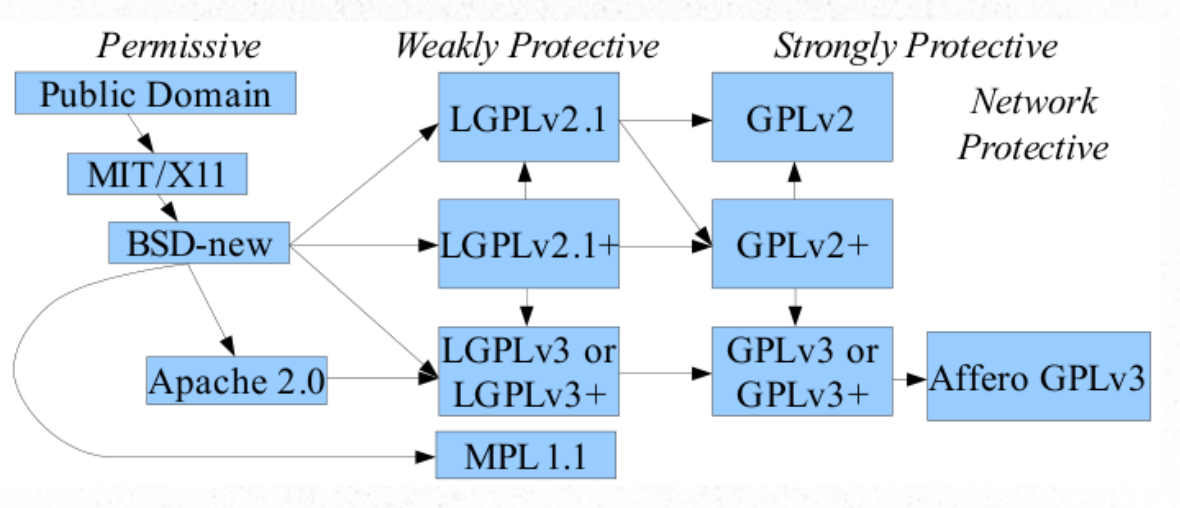
\includegraphics[width=100mm]{images/license-compatibility.png}
\caption{Mappa di compatibilità delle licenze}
\end{figure}

\section{Riassunto}

\begin{itemize}
	\item \textbf{MIT}: fai quello che vuoi, ma fornisci anche la licenza originale
	\item \textbf{BSD2}: MIT + pubblica anche la documentazione, sia per il codice che per la parte binaria
	\item \textbf{BSD3}: BSD2 + non usare il mio nome per pubblicizzare il software
	\item \textbf{BSD4}: BSD3 + cita tutti quelli che hanno contribuito
	\item Sia MIT che BSD permettono di ri-licenziare come codice proprietario
	\item \textbf{Apache}: fai quello che vuoi, non usare il mio nome, puoi anche rendere il software proprietario, specifica però che hai usato SW licenziato Apache
		\begin{itemize}
			\item \textbf{1.0}: Devi cambiare il nome del software
			\item \textbf{1.1}: Pubblicizza la licenza sulla documentazione
			\item \textbf{2.0}: Devi concedere l’uso dei brevetti
		\end{itemize}
	\item \textbf{Academic Free License}: Simile alla BSD3 ma permette di rendere il codice proprietario. Garantisce la tutela dei brevetti e dei marchi del licenziante.
	\item \textbf{GPL}:
		\begin{itemize}
			\item \textbf{v2}:
				\begin{itemize}
					\item \textbf{Copia non modificata}: ripubblica con la stessa licenza, senza restrizioni tecnologiche e fornendo anche i sorgenti.
					\item \textbf{Copia modificata}: come prima + specifica che cosa hai modificato, fornisci tutto il necessario per compilare
					\item \textbf{Libertà o morte}: se non puoi rispettare le clausole di libertà, non puoi distribuire il software
					\item Il software derivato da GPLv2 non può essere rilasciato sotto una licenza più restrittiva
				\end{itemize}
			\item \textbf{LGPLv2}: Programmi non liberi possono usare il codice, ma devono mantenere la libreria sotto la stessa licenza. Deve essere permesso il reverse engineering del programma non libero
			\item \textbf{v3}:
				\begin{itemize}
					\item \textbf{TiVo}: assieme ad apparecchi hardware che utilizzano software GPL devo fornire tutto il necessario per compilare il codice modificato. Anche eventuali chiavi crittografiche. Fatta eccezione per i casi in cui il fatto che il programma non può essere modificato è importante (apparecchi commerciali)
					\item \textbf{Brevetti}: chi pubblica sotto GPL concede anche la licenza d’uso dei brevetti
					\item \textbf{DMCA/DRM}: chiunque può aggiungere e togliere le protezioni DRM a codice GPL
				\end{itemize}
			\item \textbf{AGPLv3}: GPLv3 + codice disponibile su server per le applicazioni web
		\end{itemize}
	\item \textbf{MPL}: simil-GPL ma applicata file per file. Così posso integrare al programma anche codice proprietario. Va bene anche per i brevetti. Licenza chiave per Netscape.
	\item \textbf{Perl Artistic License}:
		\begin{itemize}
			\item Ridistribuzione del sorgente modificato:
				\begin{itemize}
					\item specificare che file ho modificato e come li ho modificati
					\item rilascio nel dominio pubblico oppure cambio il nome specifico le differenze oppure ne faccio uso privato
				\end{itemize}
			\item Ridistribuzione dei binari modificati possibile ma devo specificare dove posso recuperare la versione standard
			\item Posso commercializzare il prodotto modificato, però non posso venderlo direttamente, ovvero posso integrarlo in software commerciale oppure posso vendere il supporto tecnico.
		\end{itemize}
\end{itemize}


	\chapter{Open Content}

\section*{Materiale di riferimento}

\begin{itemize}

\item \textit{Viral Spiral, How the Commoners Built a Digital Republic of Their Own} - David Bollier;

\url{http://www.viralspiral.cc/sites/default/files/ViralSpiral.pdf}

\item La licenza GFDL 

\url{https://it.wikipedia.org/wiki/GNU_Free_Documentation_License};
\item \textit{Creative Commons: a user guide} - Simone Aliprandi

 \url{http://www.aliprandi.org/cc-user-guide/}.
\end{itemize}

\section*{Per approfondire}

\begin{itemize}
\item \textit{EFF} - Wikipedia 

\url{https://it.wikipedia.org/wiki/Electronic_Frontier_Foundation}
\item \textit{EFF Official Website}

 \url{https://www.eff.org/}
\item \textit{Il caso Sega vs Accolade} - Wikipedia 

\url{https://en.wikipedia.org/wiki/Sega_v._Accolade}
\item \textit{Scarichiamoli} 

\url{ttp://www.scarichiamoli.org}
\item \textit{The Economy of Ideas} - John Perry Barlow 

\url{http://www.wired.com/1994/03/economy-ideas/}
\item \textit{A Declaration of the Independence of Cyberspace} - John Perry Barlow 

\url{https://projects.eff.org/~barlow/Declaration-Final.html}
\item \textit{Dichiarazione d'indipendenza del Cyberspazio} - John Perry Barlow 

\url{http://www.olografix.org/loris/open/manifesto_it.htm}
\item \textit{Eric Eldred} -  Wikipedia

\url{https://en.wikipedia.org/wiki/Eric_Eldred}
\item \textit{Eldred v. Ashcroft} -  Wikipedia 

\url{https://en.wikipedia.org/wiki/Eldred_v._Ashcroft}
\item \textit{Righting Copyright} 

\url{http://www.bookforum.com/archive/feb_05/boynton.html}
\end{itemize}

\section{I primi tentativi}

La \textbf{GNU Free Documentation License} è partita all'inizio perché c'era la necessità di avere una \textbf{documentazione libera}. Per molto tempo la documentazione che accompagnava il software libero era sotto licenza GPL e lo stesso TLDP (The Linux Documentation Project) distribuiva la sua documentazione sotto GPL, semplicemente perché era quello che ``passava al convento'', ma non ha molto senso usare la GPL per della documentazione. Se per esempio i \textit{Promessi Sposi} fosstrasparentiero sotto licenza GPL io potrei prendere i sorgenti e cambiare nella copertina il nome dell'autore: questo posso farlo tranquillamente senza problemi se sono sotto GPL. Ma questo è un problema perché c'è differenza tra protezione del software e protezione del contenuto testuale. La tutela dell'autore originale è importante. Per questo motivo la GNU Free Documentation License si è posta come obiettivo una documentazione che avesse:

\begin{itemize}

\item Libertà di modifica;
\item Tutele dei diritti morali dell'autore;
\item Gestione del problema legato alle copie non trasparenti; come nel caso della GPL si vuole far sì che se qualcuno modifica un prodotto che è sotto GFDL quello rimanga disponibile nei suoi sorgenti (ad esempio non posso redistribuire un documento come serie di immagini jpeg che non sono editabili) e che non limiti la libertà di terzi di modificare la documentazione;
\item Copia in grande quantità e non.

\end{itemize}

\section{Concetti fondamentali}

È una licenza che nasce per la \textbf{documentazione} (soprattutto del progetto GNU). Si sente la necessità di dare al prodotto la possibilità di avere una documentazione sempre aggiornata quando esso viene rilasciato. Se ad esempio attuo una modifica al programma è necessario modificare la documentazione che ci sta dietro. 

Le parti del documento da considerare sono:

\begin{itemize}

\item Il \textbf{titolo}; se io modifico un documento sotto GFDL devo mantenere l'autore originale nella copertina aggiungendo eventualmente il mio;
\item Il documento in sè e il suo \textbf{contenuto};
\item \textbf{Sezioni secondarie e invarianti}, come ad esempio le dediche che possono essere modificate solamente mantenendo inalterato il tono. Le sezioni invarianti non possono assolutamente essere modificate ma devono essere al di fuori dell'argomento principale del documento;
\item \textbf{Testi di copertina}; posso modificare la copertina ma devo dichiararmi editore di quella versione;
\item \textbf{Storia del documento}, devo tenere traccia di tutte le modifiche e scriverle in una sezione del documento (esempio sezione Diario delle Modifiche);
\item La \textbf{licenza} dev'essere mantenuta e riportata nel documento.

\end{itemize}

Per quanto riguarda le copie trasparenti ci sono distinzioni per chi distribuisce sotto piccola quantità e grande quantità. In particolare se io voglio pubblicare un documento sul mio sito devo renderlo accessibile. Inoltre non devo aggiungere delle \textbf{restrizioni tecnologiche} che impediscano la modifica. 

Esiste tutta una serie di restrizioni per quanto riguarda la redistribuzione di \textbf{copie senza modifiche}:

\begin{itemize}

\item Mantenimento della licenza;
\item Nessuna misura tecnologica di restrizione;
\item Permettere di esibire la copia in pubblico;
\item Per quanto riguarda le redistribuzioni voluminose:
	\begin{itemize}

	\item Obbligo di identificarsi come autore;
	\item Obbligo di mantenere titoli e testi di copertina;
	\item Obbligo di distribuire una sorgente trasparente.

	\end{itemize}

\end{itemize}

Per quanto riguarda la redistribuzione di \textbf{copie modificate}:

\begin{itemize}

\item Devo modificare il titolo, in questo modo identifico il mio prodotto come qualcosa di diverso;
\item Indicazione degli autori delle modifiche e del documento originale;
\item Rimozione e/o aggiunta dei ``riconoscimenti'';
\item Aggiornamento della sezione cronologia;
\item Preservazione degli invarianti;
\item Preservazione della versione trasparente;
\item Preservazione e/o aggiunta dei testi di copertina.

\end{itemize}

Esistono anche tutta una serie di paragrafi di questa licenza che parlano essenzialmente dell'\textbf{unione di documenti}, delle collezioni e aggregati e delle \textbf{traduzioni} dei documenti. Per quanto riguarda le unioni di più documenti è necessario:

\begin{itemize}

\item Disambiguare tutte le parti;
\item Mantenere una licenza;
\item Rimuovere i riconoscimenti.

\end{itemize}

Un caso particolare è quando si tratta delle traduzioni: la traduzione è comunque considerata una modifica e in questo caso è necessario conservare la licenza e allo stesso tempo conservare gli invarianti. In questo modo si da garanzia all'autore che la sua opera non possa venire mal interpretata perché io potrei tradurla in maniera non appropriata (scritta male o con ambiguità). È possibile in ogni caso prendere accordi con l'autore.

\section{Il fallimento del copyright}

C'è stato un cambiamento enorme per quanto riguarda i tipi di diritti associati agli utenti e agli sviluppatori del software. 

\section{Gli anni d'oro della proprietà intellettuale}
\subsection{Il caso Nation - Ford}

Il presidente Gerald Ford scrisse una biografia includendo un anedotto sulla sua decisione di perdonare Richard Nixon. 
Ford aveva concesso sotto licenza i suoi diritti di pubblicazione alla Harper\&Row con un contratto per pubblicare un estratto delle memorie sul magazine \virg{Time}. 
Invece, la rivista \virg{The Nation} pubblicò dalle 300 alle 400 citazioni letterali direttamente dal libro di 500 pagine senza il permesso né di Ford, né della Harper\&Row né del Time.
Vista questa pubblicazione anticipata, il Time si tirò indietro dal contratto (il che era permesso da una clausola) e la Harper\&Row intentò una causa legale contro The Nation.\\

The Nation affermò che essendo Ford un personaggio pubblico e che le informazioni da lui divulgate fossero di vitale importanza la pubblicazione ricadesse sotto il fair use.\\

Un primo verdetto diede ragione alla Harper\&Row, ma uno successivo
della corte d'appello ribaltò la sentenza a favore di The Nation. Harper\&Row ricorse alla corte suprema, la quale ribaltò di nuovo il
verdetto, stabilendo che il fair use non è una difesa in caso di  
pre-pubblicazione e non permette l'appropriazione commerciale del 
lavoro di un famoso personaggio politico semplicemente 
a causa del pubblico interesse nell'apprendere informazioni su una
figura politica di un evento storico.\\

\begin{sloppypar}\tolerance=9999
\url{https://en.wikipedia.org/wiki/Harper_%26_Row_v._Nation_Enterprises}
\end{sloppypar}

\subsection{I ruoli di Kastenmeier e Schrader}

Robert Kastenmeier fu un politico americano membro del partito democratico. 
Dorothy Schrader fu consigliere generale per il Copyright Office degli Stati Uniti entrambi diedero un significativo contributo al Copyright Act del 1976.

\section{I prodromi della crisi}

Con l'avanzare di internet negli anni '90, il boom delle vendite di apparecchi elettronici e i film su videocassette si ha una contrapposizione tra utenti e lobby pro proprietà intellettuale che si fanno ancora più aggressive, arrivando a brevettare pressoché tutto (persino forme di vita come semi per l'agricoltura).

Dal punto di vista del software nello stesso periodo nasce l'EULA (\textit{End-User Licence Agreement}), un contratto tra il fornitore di un programma software e l'utente finale. Tale contratto assegna la licenza d'uso del programma all'utente nei termini stabiliti dal contratto stesso e nel 1990 nasce EFF (\textit{Electronic Frontier Foundation}) un'organizzazione internazionale non profit di avvocati e legali rivolta alla tutela dei diritti digitali e della libertà di parola nel contesto dell'odierna era digitale e il \textit{Berkman Center} un'istituto dell'università di Harvard dedicato allo studio e alla comprensione del Cyberspazio definendo e studiando norme, dinamiche e standard \url{https://cyber.law.harvard.edu/}

Tornando ai brevetti, nel 1999 Amazon arrivò a brevettare negli USA gli acquisti One-click (brevetto rifiutato nell'Unione Europea a causa di un mancato processo inventivo).

Negli anni '90 fece molto discutere il caso \textit{SEGA - Accolade}. Accolade casa produttrice e rivenditore di videogiochi, disassemblò tramite tecniche di Reverse Engineering alcuni giochi per la console Genesis di SEGA, in modo da poter pubblicare giochi compatibili per la console di SEGA senza il loro consenso. Il caso fece molto parlare di se visto che riguardava vari aspetti controversi come il copyright, l'uso permissivo di marchi e il fair use applicato al codice.
Nel 1992 SEGA vinse e Accolade fu costretta ad interrompere la produzione di giochi compatibili e a ritirare le copie dal mercato, Accolade ricorse in appello e il 28 agosto 1992 vinse (anche a seguito di forti pressioni da varie associazioni e del clamore mediatico del caso), quando la corte d'appello stabilì che la decompilazione ricadeva nel fair-use e condannò per altri motivi SEGA al pagamento di tutte le spese processuali. Alla fine le due compagnie trovarono un accordo conveniente ad entrambe. Il caso servì a stabilire che i principi funzionali del software non possono essere protetti da diritti d'autore (non e' possibile brevettare un algoritmo) e la corte incoraggiò la copia di software protetto per l'esplorazione di funzionalità non protette.\\

Altro evento importante fu l'approvazione da parte dell'amministrazione Clinton del \textit{National Information Infrastructure (NII)} un insieme di regole atte a costruire reti di comunicazione, servizi interattivi, hardware e software interattivo, per rendere disponibile sia al settore pubblico che privato una marea di informazione senza favorire un'azienda sull'altra. Purtroppo vennero anche introdotte ulteriori restrizioni, come la rimozione dei diritti di prima vendita e il DRM.

\section{Il movimento degli accademici}

Molti accademici nel mondo legale come Peter Jaszi e Lawrence Lessig iniziarono ad approfondire la questione legale attorno alla libertà d'espressione, il fair use e il copyright. In particolare Peter Jaszi fondò nel 1995 la \textit{Digital Future Coalition (DFC)} , un'organizzazione legale americana volta a trovare un giusto equilibrio tra salvaguardia della proprietà intellettuale e il libero accesso alla cultura e all'informazione. In particolare la DFC si oppose al white paper di Bruce Lehman in merito al NII e alle sue misure restrittive e al DMCA del 1998. Attualmente la DFC conta 42 altri enti e associazioni aderenti.\\

Nel 1994 venne pubblicato da John Perry Barlow \textit{The Economy of Ideas}, un articolo provocante qui riassunto in quattro punti:
\begin{itemize}
\item Le leggi sul copyright non si adattano bene a proprietà che possono essere infinitamente riprodotte e distribuite istantaneamente.
\item Le opere assumono valore nella trasmissione, l'informazione assume importanza se condivisa.
\item I beni intellettuali diventano sempre più prominenti ma proteggerne la proprietà è sempre più difficile.
\item Indifferenza sociale nei confronti della pirateria.
\end{itemize}
Sempre lo stesso autore pubblicherà nel 1996 un altro famoso manifesto \textit{La dichiarazione d'indipendenza del Cyber spazio}

Insomma a fine anni '90 vengono gettate le basi per licenze permissive, Authorship collettive (come wikipedia) e il dominio pubblico viene visto come una fonte di crescita, personale e sociale.

\section{Mickey Mouse Protection Art}

Nel 1998 venne approvato il \textit{Sonny Bono Copyright
Extension Act (SBCEA)} che estese di 20 anni i termini di protezione per le opere registrate dopo il 1923 negli USA. Il Sonny Bono Act prende il nome da un cantante che la appoggiò fortemente (salvo poi mai vederla approvata, visto che morì prima). La legge è anche conosciuta con il nome Mickey Mouse Protection Act, dal momento che la Disney ebbe un ruolo significativo nelle azioni di lobbismo per approvare la legge. Ogni volta che i diritti inerenti il personaggio di Topolino stanno per scadere, puntualmente viene approvata una legge per estendere la durata del copyright, come mostrato dal seguente grafico:

\begin{figure}[htbp]
\centering
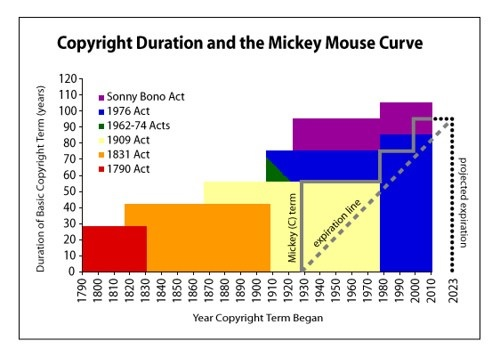
\includegraphics[width=50mm]{images/MM_copyright_graph}
\caption{Leggi sull'estensione del copyright e Topolino}
\end{figure}

\section{Eldred vs Reno}

Eric Eldred aveva fondato la Eldritch Press, un sito e casa editrice che pubblicava opere divenute di dominio pubblico appena scadevano i diritti d'autore, con l'approvazione del Sonny Bonno Act divenne impossibile proseguire il lavoro per le opere pubblicate dopo il 1922. \\

La sua storia si intrecciò a quella di Lessig. Lessig, giovane avvocato e attivista politico era interessato alla legge come strumento di cambiamento politico e all'impatto della società sulla legge. I due strinsero quindi un patto che sfociò nel dibattimento Eldred vs Reno con l'obiettivo di denunciare l'incostituzionalità del SBCEA, purtroppo i due persero davanti alla corte suprema nel 2003, la quale stabilì che l'estensione retroattiva di vent'anni del copyright esistente non violava la clausola del diritto d'autore o il Primo emendamento della Costituzione degli Stati Uniti d'America.  Il caso ebbe comunque un'ampia risonanza e fu il primo esperimento di \textit{openlaw} con tanto di newsletter e forum nei quali l'opinione pubblica veniva informata dello svolgersi del processo e delle varie iniziative legali a tutela del dominio pubblico.\\

Se Topolino smuoveva interessi economici troppo forti i due decisero di dedicarsi ad opere minori creando un movimento tecnico - legale puntando sula copyright conservancy, portando quindi alla nascita di Creative Commons.

\section{Creative Commons}
La nascita di Creative Commons passò prima per vari step

\begin{itemize}
\item 1999: nasce Copyright Commons diretto da Jennifer Love e Ashley Morgan, una newsletter mensile sul caso Eldred vs Reno e varie news sul public domain

\item Nasce la Campagna Counter Copyright (CC): Ponendo l'icona CC (il counter-copyright) alla fine dell'opera, l'autore segnala agli altri che permette di usare, modificare, adattare e ridistribuire il suo lavoro. Il Counter Copyright non è un rimpiazzo al copyright attuale, è solo un segnale che l'autore permette agli altri di condividere il suo lavoro. 
Però il Counter Copyright strappò via al copyright l'esclusività di fornire e autorizzare altre persone per l'uso di un'opera per le loro opere creative.

\item 1999: Napster incontra i talk di Lessig

\item 2000 - Abelson ha l'idea di  una fondazione che accetti donazioni di opere

\item 2001: viene fondato Creative Commons, un'organizzazione statunitense non profit dedicata ad ampliare la gamma di opere creative disponibili alla condivisione e all'utilizzo pubblico in maniera legale. Rende possibile il riuso creativo di opere dell'ingegno altrui nel pieno rispetto delle leggi esistenti.
Il nome nasce da un gioco di parole sulla “tragedia dei beni comuni”
di Garret Hardin \url{https://it.wikipedia.org/wiki/Tragedia_dei_beni_comuni}

\item 2003: nasce il distaccamento italiano
\end{itemize}

\subsection{Obiettivi}
\begin{itemize}
\item Promuovere la diffusione di un modello “alcuni diritti riservati”

\item Tutelare il marchio “Creative Commons”

\item Creazione di appropriati strumenti legali e tecnologici
\end{itemize}

Il tutto senza essere né un ente pubblico, né organismo per la raccolta dei diritti d'autore e soprattutto senza offrire servizi di consulenza legale.

\section{Le licenze Creative Commons}

Creative Commons permette agli utenti di rilasciare il loro lavoro scegliendo tra varie licenze pensate per opere creative (non software) disponibili per 52 sistemi giuridici permettendo di 

\begin{itemize}
\item Preservare delle note di licenza
\item Copiare e distribuire l'opera
\item Esibire l'opera o convertirla di formato
\end{itemize}

E vientando l'uso di restrizioni tecnologiche.

Ogni licenza si compone di tre parti:
\begin{itemize}
\item \textbf{Commons Deed}: una sintesi del contratto comprensibile a chiunque tramite un breve riassunto e dei simboli facilmente comprensibili e riconoscibili. I 4 simboli combinabili tra loro sono:

\begin{figure}[htbp]
\centering
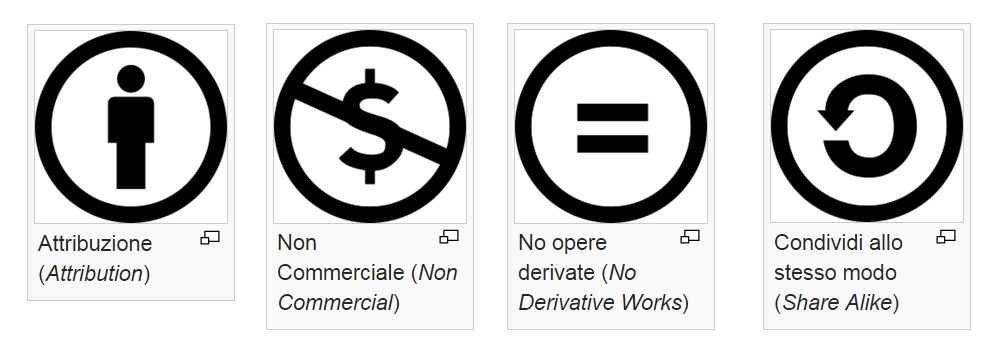
\includegraphics[width=50mm]{images/CC_Deed}
\caption{Le quattro clausole base delle Licenze CC}
\end{figure}

Condividi allo stesso modo (Share Alike - SA) e No Opere derivate (ND) non possono essere combinati tra loro

\item \textbf{Legal Code}: l’intero contratto espresso in linguaggio tecnico-giuridico in base al paese scelto. E' la licenza vera è propria.
\item \textbf{Digital Code}: Metadati che descrivono gli elementi chiave della licenza, applicando all'opera un codice che la rende ricercabile dai motori di ricerca abilitati.
\end{itemize}

\subsection{Le sei licenze}
Le sei licenze CC sono:

\begin{wrapfigure}{L}{0.15\textwidth}
    
\includegraphics[width=20mm]{images/cc_by}
\end{wrapfigure}

\noindent \textbf{Attribuzione CC BY} Questa licenza permette a terzi di distribuire, modificare, ottimizzare ed utilizzare l' opera come base, anche commercialmente, fino a che sia riconosciuto il credito per la creazione originale all'autore. Questa è la più accomodante delle licenze offerte ed è raccomandata per la diffusione e l'uso massimo di materiali coperti da licenza.\\
\begin{wrapfigure}{L}{0.15\textwidth}
    
\includegraphics[width=20mm]{images/cc_by_sa}
\end{wrapfigure}

\noindent \textbf{Attribuzione - Condividi allo stesso modo CC BY-SA} Estende la precedente permettendo la redistribuzione anche a scopo commerciale e autorizza le loro nuove creazioni con i medesimi termini. Questa licenza è spesso comparata con le licenze usate dai software opensource e gratuite "copyleft". Tutte le opere basate sull'originale porteranno la stessa licenza, quindi tutte le derivate permetteranno anche un uso commerciale. Questa è la licenza usata da Wikipedia, ed è consigliata per materiali che potrebbero beneficiare dell'incorporazione di contenuti da progetti come Wikipedia e similari.\\

\begin{wrapfigure}{L}{0.15\textwidth}
    
\includegraphics[width=20mm]{images/cc_by_nd}
\end{wrapfigure}

\noindent \textbf{Attribuzione - Non opere derivate CC BY-ND} Questa licenza permette la ridistribuzione, commerciale e non, fintanto che viene trasmessa intera ed invariata, dando credito all'autore. Non permette tuttavia la creazione di opere derivate.\\

\begin{wrapfigure}{L}{0.15\textwidth}
    
\includegraphics[width=20mm]{images/cc_by_nc}
\end{wrapfigure}

\noindent \textbf{Attribuzione - Non commerciale CC BY-NC} Questa licenza permette a terzi di modificare, ottimizzare ed utilizzare l' opera come base per altre non commerciali, anche le opere derivate dovranno essere non commerciali.\\

\begin{wrapfigure}{L}{0.15\textwidth}
    
\includegraphics[width=20mm]{images/cc_by_nc_sa}
\end{wrapfigure}

\noindent \textbf{Attribuzione - Non commerciale - Condividi allo stesso modo CC BY-NC-SA} Questa licenza permette a terzi di modificare, redistribuire, ottimizzare ed utilizzare l'opera come base non commerciale, fino a che riconoscano i crediti all'autore e licenzino le loro nuove creazioni mediante i medesimi termini.\\

\begin{wrapfigure}{L}{0.15\textwidth}
    
\includegraphics[width=20mm]{images/cc_by_nc_nd}
\end{wrapfigure}

\noindent \textbf{Attribuzione - Non commerciale - Non opere derivate 
CC BY-NC-ND} Questa licenza è la più restrittiva delle sei principali, permettendo a terzi soltanto di scaricare le opere e condividerle ad altri fino a che riconoscano i giusti crediti, ma non possono cambiarle in nessun modo od utilizzarle commercialmente.\\

Le licenze sono pensate anche per trattare lavori collettivi (dove l'opera è parte di una più ampia) e opere derivate e permettono la distribuzione della licenza e delle clausole di salvaguardia anche attraverso url.\\

Devono includere:
\begin{itemize}
\item La citazione dell'autore originario, rimovibile su richiesta del licenziante
\item Titolo dell'opera originaria
\item Se possibile url associato all'opera
\item Uso dell'opera
\end{itemize}

\section{Altri strumenti}

Creative Commons oltre alle licenze sopra descritte fornisce anche altri strumenti utili agli autori:\\

\begin{wrapfigure}{L}{0.15\textwidth}
    
\includegraphics[width=20mm]{images/CC0}
\end{wrapfigure}

\noindent \textbf{CC0} Un'alternativa al dominio pubblico, il detentore dei diritti d'autore può rinunciare a tutti i suoi interessi sulla sua opera.\\ \\

\begin{wrapfigure}{L}{0.15\textwidth}
    
\includegraphics[width=20mm]{images/cc_PD}
\end{wrapfigure}

\noindent \textbf{Marchio di pubblico dominio} Per marcare opere libere da restrizioni di copyright\\

\textbf{CC plus (CC+)} Un protocollo \glossario{RDF} per esprimere licenze alternative, è possibile combinare le licenze CC con altre separate ed indipendenti che diano più diritti, senza però modificare il legal code originale.\\

\textbf{Founders Copyright} Non più supportato, permetteva agli autori di detenere i diritti per l'opera per 14 anni e poi questa diveniva di pubblico dominio. Si ispirava alle leggi sul diritto d'autore in vigore nel 1790, senza cambiare nessuna legge in vigore aiutava i detentori di diritti che ritenessero troppo lungo il periodo di 70 anni, di rilasciare le opere dopo un periodo molto più corto.

\subsection{Link utili}

E' possibile scegliere una licenza CC all'indirizzo: \\

\url{https://creativecommons.org/choose/}\\

Mentre per usare CC0 il link è il seguente: \\

\url{https://creativecommons.org/choose/zero/waiver}\\

compilando un semplice form online.\\

E' inoltre possibile ricercare opere poste sotto licenze CC al link \\

\url{http://search.creativecommons.org/}.\\

\section{Scarichiamoli}

Scarichiamoli è un progetto creato all'interno di Creative Commons
Italia: \\

\url{http://www.scarichiamoli.org/main.php} \\

Le opere di ingegno finanziate a fondo perduto con soldi pubblici dovrebbero essere:

\begin{itemize}
\item Pubblicamente accessibili: facilmente reperibili su Internet
\item Universalmente accessibili: accessibili anche per i diversamente abili
\item Liberamente fruibili: non occorre pagare per: leggere un testo, vedere un'immagine, ascoltare una musica
\item legalmente fruibili: (l'utente è certo di poter scaricare un file nella piena legalità)
\item ottimamente fruibili (qualità digitale idonea a garantire una buona visualizzazione e/o un buon ascolto)
\end{itemize}
	\chapter{RDF}

Il \textbf{R}esource \textbf{D}escription \textbf{F}ramework è un linguaggio definito dal W3C per rappresentare informazioni semantiche sul web.

Le informazioni modellate con RDF sono strutturate secondo delle ontologie o dizionari: raccolte di classi e proprietà utili per descrivere un determinato contesto. Alcuni esempi di dizionari sono:

\begin{itemize}
	\item \textbf{Dublin Core} (dc):  un dizionario che contiene i termini per descrivere risorse multimediali e fisiche, come foto, video, libri, ecc.
	\item \textbf{Friend of a Friend} (foaf): un dizionario che contiene i termini per descrivere le reti sociali
	\item \textbf{Creative Commons Rights Expression Language} (ccREL): un dizionario per descrivere le informazioni riguardo la licenza con cui vengono pubblicati i contenuti multimediali che sono sotto licenze Creative Commons. Questi termini sono predisposti per essere inseriti all'interno di una pagina web utilizzando RDFa.
\end{itemize}

\noindent Queste informazioni vengono poi raggruppante e codificate in vario modo, un dei tanti è utilizzando \textbf{RDFa}, una serie di tag \textit{xhtml} che permetto di inserirle direttamente all'interno di una pagina web.

\section{Che cos'è RDF?}

RDF è un linguaggio di modellazione simile a quello ER o ai diagrammi delle classi, che si basa sulla definizione di \textbf{statement} (asserzioni) riguardanti delle \textbf{resources} nella forma \textit{soggetto-predicato-complemento}, con l'obiettivo che siano facilmente interpretabili sia da una persone che da un computer.

Ad esempio l'affermazione \textit{``il cielo è azzurro''} con RDF viene descritta come:

\begin{itemize}
	\item \textbf{Soggetto}: il cielo
	\item \textbf{Predicato} è di colore
	\item \textbf{Oggetto}: azzurro
\end{itemize}

Quando vengono descritte informazioni più complesse, può essere che un soggetto sia anche l'oggetto di altri statement, si parla quindi di:

\begin{itemize}
	\item \textbf{Risorse}: sono identificate da un URI e possono funzionare sia da soggetto che da oggetto. Possono anche essere definiti dei nodi anonimi con la sintassi \texttt{\_:\textit{identificatoreDelNodo}}.
	\item \textbf{Letterali}: un valore stringa primitivo che funziona solamente da oggetto. Utilizzando XSD è possibile specificare tipi diversi, come \texttt{xsd:integer} e \texttt{xsd:boolean}.
	\item \textbf{Proprietà}: il predicato della frase. Descrive un attributo o un aspetto di una risorsa e il valore della proprietà può essere sia un'altra risorsa che un letterale. Anche in questo caso è identificata da un URI. 
\end{itemize}

Un \textbf{URI} non è altro che un nome che viene dato ad una risorsa che si trova nel web e la scelta dell'URI da utilizzare viene lasciata all'utente.
Ad esempio per indicare la classe di vini Merlot è possibile utilizzare l'URI:

\begin{center}
	\texttt{http://www.w3.org/TR/2004/REC-owl-guide-20040210/wine\#Merlot}
\end{center}

Da notare che non è obbligatorio utilizzare un URL, ma se si vuole creare uno dizionario pubblico per descrivere una determinata categoria di informazioni. Nell'esempio precedente l'URL porta alla definizione del dizionario \texttt{wine}.

Dato che gli URI possono essere molto lunghi e quindi possono rendere il documento di difficile comprensione è possibile utilizzare gli XML Qualified Name per creare un namespace.
Ad esempio l'URI precendete può essere abbreviato con 

\begin{center}
	\texttt{wine : http://www.w3.org/TR/2004/REC-owl-guide-20040210/wine}
\end{center}

\noindent così facendo ci si può riferire al Merlot utilizzando solamente \texttt{wine:Merlot}.

\subsection{Rappresentazione dei dati RDF}

Ci sono vari modi per rappresentare dati in formato RDF.
Come esempio per confrontare le varie sintassi viene utilizzata la frase:

\begin{center}
	\textit{C'è una persona identificata da \texttt{http://www.w3.org/People/EM/contact\#me}, che si chiama Eric Miller, che ha come indirizzo email e.miller123(at)example  e che ha il titolo di Dr.}
\end{center}

In questo caso si ha che gli oggetti sono: \textit{``Eric Miller''}, \textit{mailto:e.miller123(at)example} e \textit{``Dr.''}. L'unico soggetto è un URI e i vari predicati sono anch'essi identificati da un URI:

\begin{itemize}
	\item \textit{si chiama} : \texttt{http://www.w3.org/2000/10/swap/pim/contact\#fullName}
	\item \textit{ha come indirizzo email} : \texttt{http://www.w3.org/2000/10/swap/pim/contact\#mailbox}
	\item \textit{ha il titolo di} : \texttt{http://www.w3.org/2000/10/swap/pim/contact\#personalTitle}
\end{itemize}

Inoltre viene anche espresso il fatto che il soggetto ha un determinato tipo che è \textit{Persona}.

\subsubsection{N-Triple e Turtle}

Il formato più semplice per descrivere i dati in formato RDF è \textbf{N-Triple}, il quale consiste in un file di testo UTF-8 le cui linee o sono dei commenti che iniziano con \texttt{\#} oppure seguono la sintassi

\begin{center}
	\texttt{soggetto predicato complemento .}
\end{center}

La frase d'esempio viene rappresentata in N-Triple con:

\begin{lstlisting}
<http://www.w3.org/People/EM/contact#me> <http://www.w3.org/2000/10/swap/pim/contact#fullName> "Eric Miller" .
<http://www.w3.org/People/EM/contact#me> <http://www.w3.org/2000/10/swap/pim/contact#mailbox> <mailto:e.miller123(at)example> .
<http://www.w3.org/People/EM/contact#me> <http://www.w3.org/2000/10/swap/pim/contact#personalTitle> "Dr." .
<http://www.w3.org/People/EM/contact#me> <http://www.w3.org/1999/02/22-rdf-syntax-ns#type> <http://www.w3.org/2000/10/swap/pim/contact#Person> .
\end{lstlisting}

Una versione più avanzata di N-Triple è \textbf{Turtle} la quale permette sia di utilizzare dei prefissi per qualificare gli URI, sia di utilizzare altre notazioni avanzate.

Lo stesso esempio può essere riscritto con Turtle:

\begin{lstlisting}
@prefix eric:    <http://www.w3.org/People/EM/contact#> .
@prefix contact: <http://www.w3.org/2000/10/swap/pim/contact#> .
@prefix rdf:     <http://www.w3.org/1999/02/22-rdf-syntax-ns#> .

eric:me contact:fullName "Eric Miller" .
eric:me contact:mailbox <mailto:e.miller123(at)example> .
eric:me contact:personalTitle "Dr." .
eric:me rdf:type contact:Person .
\end{lstlisting}

\subsubsection{Rappresentazione grafica}

Le stesse informazioni possono essere rappresentate sotto forma grafica con un multi grafo orientato aciclico.

La notazione per standard per i grafi è:

\begin{itemize}
	\item \textbf{Risorse}: un ovale contenente l'URI.
	\item \textbf{Risorse anonime}: un cerchio vuoto.
	\item \textbf{Letterali}: un rettangolo contenente il valore.
	\item \textbf{Proprietà}: un arco avente l'URI della proprietà come etichetta.
\end{itemize}

\begin{figure}[htbp]
	\centering
	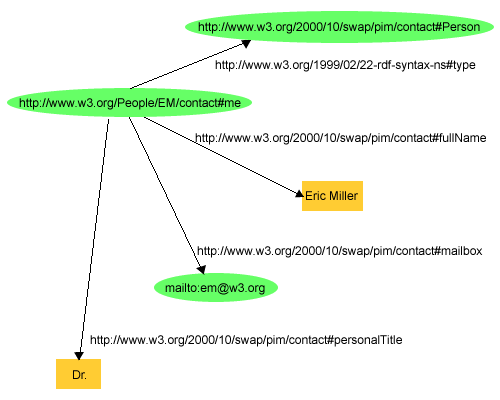
\includegraphics[width=.7\textwidth]{./images/miller_graph.png}
	\caption{Esempio di grafo RDF}
\end{figure}

\subsubsection{XML/RDF}

Esiste la possibilità di rappresentare i dati anche all'interno di un documento XML, anche se questo formato viene scarsamente utilizzato perché molto verboso e non permette di rappresentare tutti i tipi di grafi.

\begin{lstlisting}
<?xml version="1.0" encoding="utf-8"?>
<rdf:RDF xmlns:contact="http://www.w3.org/2000/10/swap/pim/contact#" xmlns:eric="http://www.w3.org/People/EM/contact#" xmlns:rdf="http://www.w3.org/1999/02/22-rdf-syntax-ns#">
	<rdf:Description rdf:about="http://www.w3.org/People/EM/contact#me">
		<contact:fullName>Eric Miller</contact:fullName>
	</rdf:Description>
	<rdf:Description rdf:about="http://www.w3.org/People/EM/contact#me">
		<contact:mailbox rdf:resource="mailto:e.miller123(at)example"/>
	</rdf:Description>
	<rdf:Description rdf:about="http://www.w3.org/People/EM/contact#me">
		<contact:personalTitle>Dr.</contact:personalTitle>
	</rdf:Description>
	<rdf:Description rdf:about="http://www.w3.org/People/EM/contact#me">
		<rdf:type rdf:resource="http://www.w3.org/2000/10/swap/pim/contact#Person"/>
	</rdf:Description>
</rdf:RDF>
\end{lstlisting}

\section{Containers e Collections RDF}

I \textbf{container} vengono utilizzati per rappresentare dei gruppi di cose, come la lista degli autori di un libro.

Ci sono 3 tipi di container:

\begin{itemize}
	\item \texttt{rdf:Bag}: rappresenta una lista non ordinata di oggetti
	\item \texttt{rdf:Seq}: rappresenta una lista ordinata di oggetti.
	\item \texttt{rdf:Alt}: rappresenta una lista di valori alternativi, dei i quali solo un può essere selezionato.
\end{itemize}
\FloatBarrier
\begin{lstlisting}[caption=Esempio di Bag con XML/RDF]
<?xml version="1.0"?>
<rdf:RDF
xmlns:rdf="http://www.w3.org/1999/02/22-rdf-syntax-ns#" 
xmlns:cd="http://www.recshop.fake/cd#"> 
	<rdf:Description rdf:about="http://www.recshop.fake/cd/Beatles">
		<cd:artist>
			<rdf:Bag>
				<rdf:li>John</rdf:li>
				<rdf:li>Paul</rdf:li>
				<rdf:li>George</rdf:li>
				<rdf:li>Ringo</rdf:li>
				</rdf:Bag>
				</cd:artist>
		</rdf:Description>
</rdf:RDF>
\end{lstlisting}

\begin{lstlisting}[caption=Bag con N-Triple]
exstaff:Sue exterms:publication _:z .
_:z rdf:type rdf:Bag .
_:z rdf:_1 ex:AnthologyOfTime .
_:z rdf:_2 ex:ZoologicalReasoning .
_:z rdf:_3 ex:GravitationalReflections . 
\end{lstlisting}

Nella rappresentazione grafica vengono utilizzate delle proprietà \textit{anonime?} con un URI che avanza progressivamente.
\FloatBarrier
\begin{figure}[htbp]
	\centering
	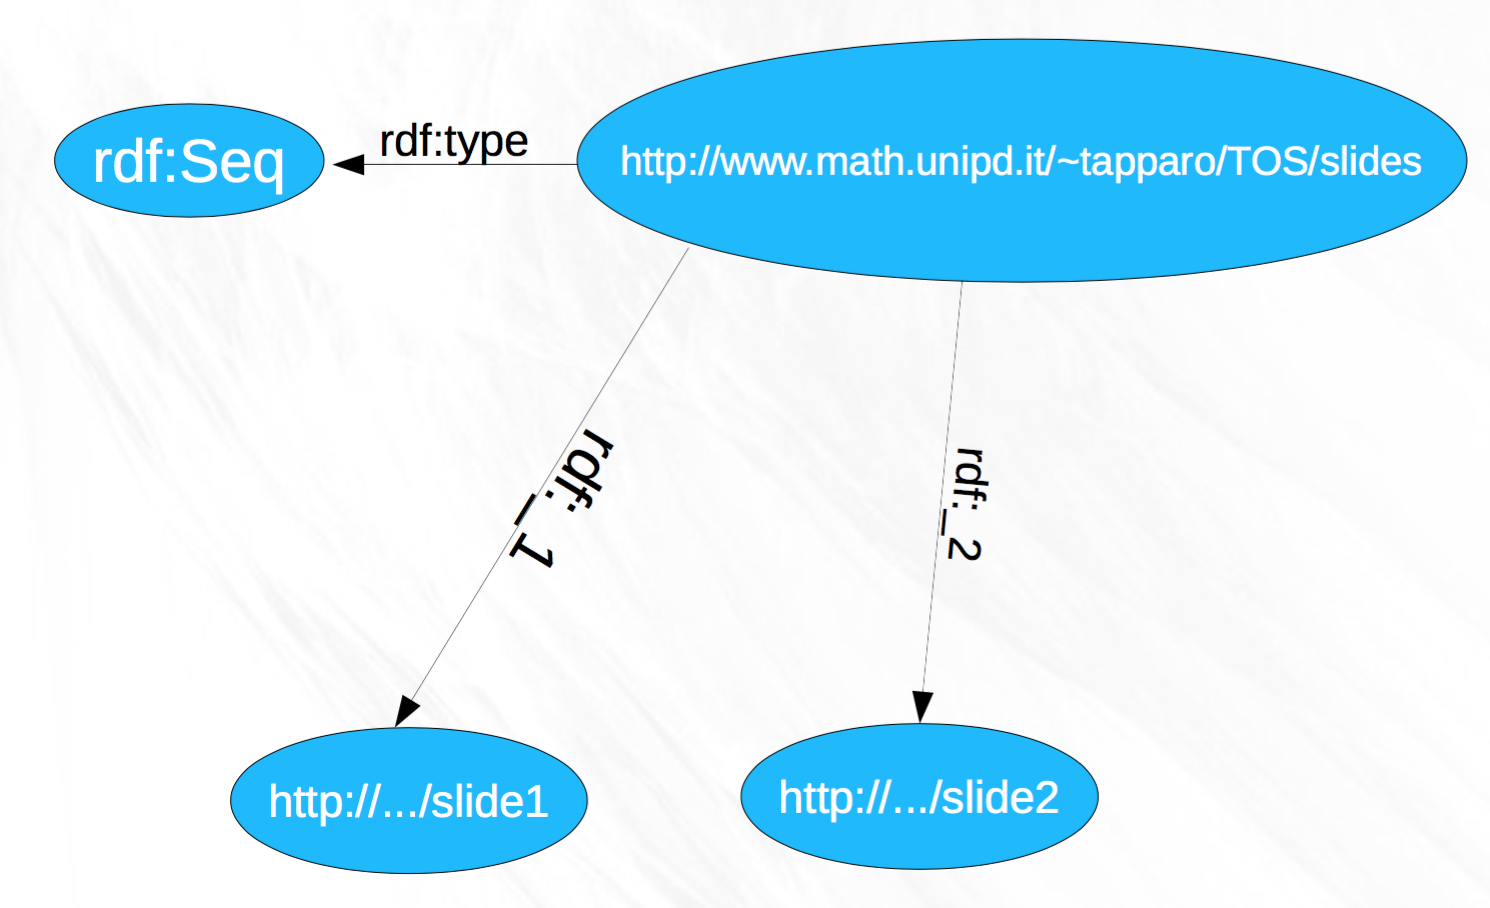
\includegraphics[width=.4\textwidth]{./images/seq_graph.png}
	\caption{Grafo RDF con \texttt{rdf:Seq}}
\end{figure}

I container però non sono bloccabili, ovvero possono essere aggiunti nuovi elementi.
Se invece si vuole limitare il numero di elementi che possono essere presenti all'interno del contenitore è necessario utilizzare una \textbf{Collection}.

Le collezioni RDF sono rappresentate come una lista singolarmente linkata e viene definita utilizzando le proprietà \texttt{rdf:first}, \texttt{rdf:rest} e \texttt{rdf:nil}.

\begin{figure}[htbp]
	\centering
	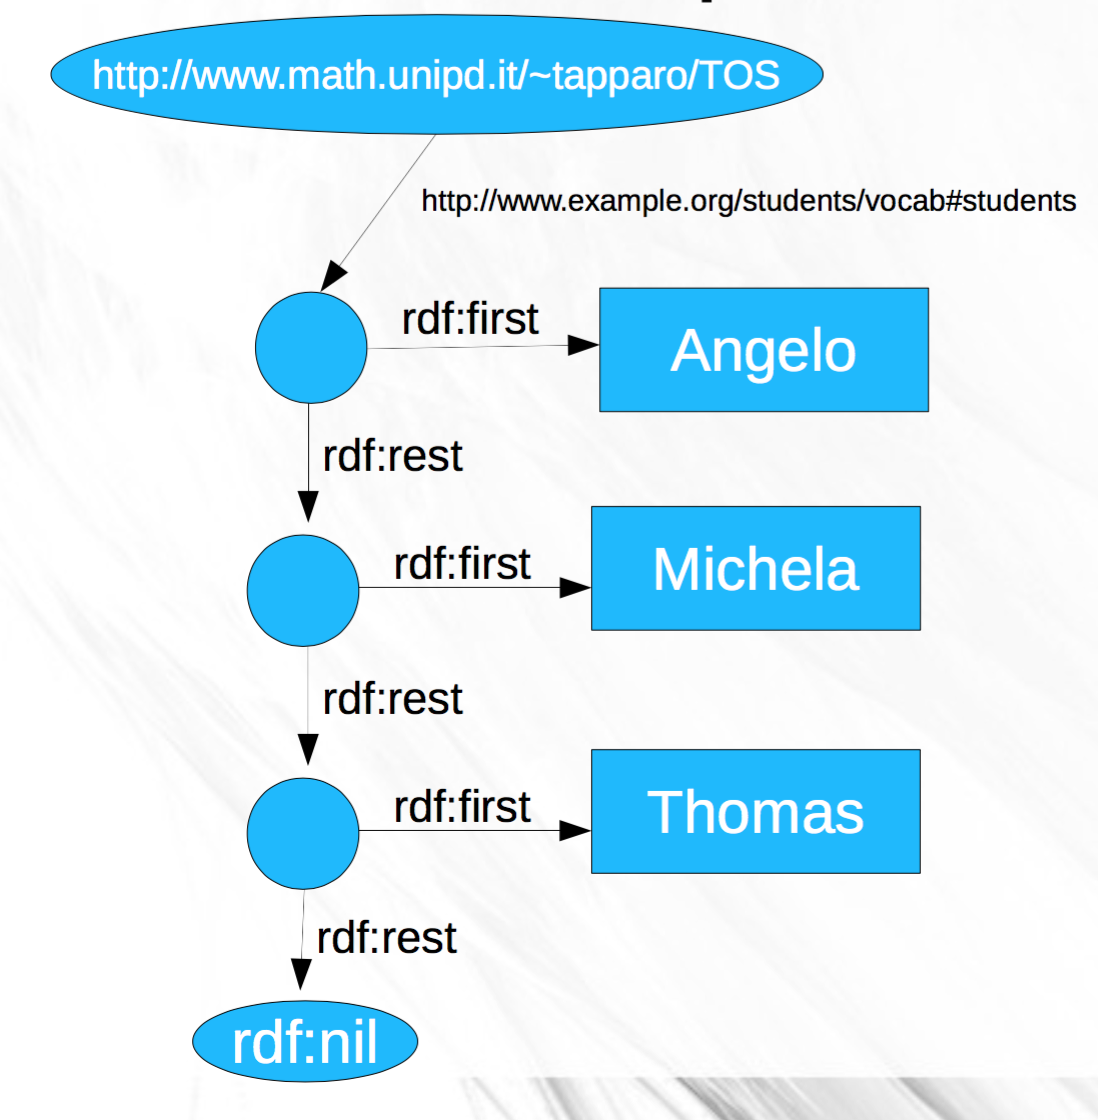
\includegraphics[width=.4\textwidth]{./images/list_graph.png}
	\caption{Grafo RDF con una collezione}
\end{figure}

La definizione di una lista con N-Triple viene fatta definendo i vari nodi:

\begin{lstlisting}[caption=Definzione di una lista con N-Triple]
http://www.math.unipd.it/~tapparo/TOS http://www.example.org/students/vocab#students _:sl
_:sl rdf:first "Angelo"
_:sl rdf:next _:sl2
_:sl2 rdf:first "Michela"
_:sl2 rdf:next _:sl3
_:sl3 rdf:first "Thomas"
_:sl3 rdf:next rdf:nil
\end{lstlisting} 

\section{Reification}

RDF permette di descrivere degli statement RDF utilizzando RDF, mediante un vocabolario built-in.

Questo vocabolario permette contiene la classe \texttt{rdf:Statement} che specifica il tipo del nodo e i predicati: \texttt{rdf:subject}, \texttt{rdf:predicate} e \texttt{rdf:object}.

Ad esempio mediante la reificazione è possibile esprimere:

\begin{center}
	\textit{Angelo ha detto che il corso di TOS è tenuto da Francesco Tapparo.}
\end{center}

\begin{lstlisting}[caption=Reification con N-Triple, language=RDFA]
# Frase detta da angelo
_:frase rdf:type rdf:Statement
_:frase rdf:subject <http://www.math.unipd.it/~tapparo/TOS/>
_:frase rdf:predicate dc:creator
_:frase rdf:object "Francesco Tapparo"

# Specifico che la farse è detta da Angelo
_:frase dc:creator _:ang
_:ang foaf:name "Angelo"
_:ang rdf:type foaf:Person
\end{lstlisting}

\begin{figure}[htbp]
	\centering
	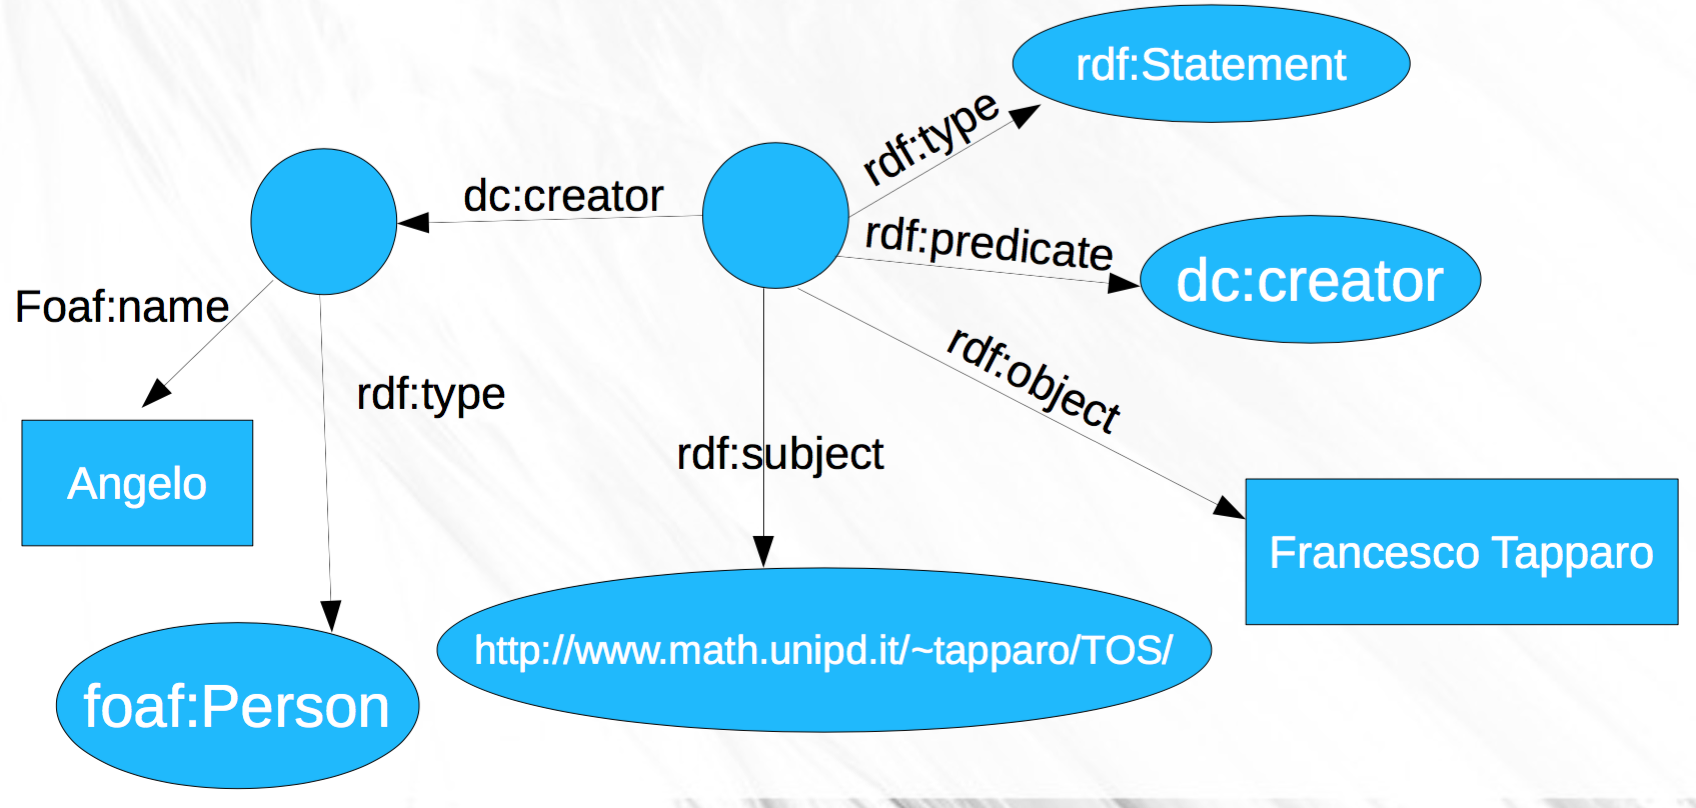
\includegraphics[width=.5\textwidth]{./images/reif_graph.png}
	\caption{Grafo RDF per: \textit{Angelo ha detto che il corso di TOS è tenuto da Francesco Tapparo.}}
\end{figure}

\section{RDFa}

RDFa è uno standard W3C che aggiunge una serie di attributi all'HTML e XHTML che permettono di inserire all'interno dei documenti i metadati RDF.

Così facendo non è più necessario mantenere un file separato con le informazioni RDF relative alla pagina web, in quanto questo può essere estratto utilizzando un distiller come \texttt{pyRdfs}\footnote{\url{https://www.w3.org/2012/pyRdfa/}}.

\subsection{Prefissi iniziali - CURIE}

Anche con RDFa è possibile utilizzare una notazione di prefissi (\textbf{CURIE}) che permette di accorciare gli URI e facilitare la comprensione all'essere umano.

Per utilizzare i prefissi basta aggiungere ad un tag la definizione del namespace, utilizzando l'attributo \texttt{xmlns}.
Una volta dichiarato il namespace, è possibile utilizzare il prefisso su tutti i tag discendenti.

\begin{lstlisting}[language=RDFA]
<html xmlns="..." xmlns:dc="http://purl.org/dc/terms/" > 
...
<!-- permette di utilizzare il prefisso dc -->
<span property="dc:description">Valore</span>

<!-- al posto di -->
<!-- property="http://purl.org/dc/terms/:description" -->
...
</html>
\end{lstlisting}

\noindent Tuttavia questo sistema utilizza i namespace XML.

Un'alternativa è quella di definire un vocabolario di default utilizzando \textbf{\texttt{vocab}} che funziona in modo simile, solo che non è possibile specificare il prefisso.
Se si vogliono utilizzare altri vocabolari è necessario specificare l'URI completo.

\begin{lstlisting}[caption=Utilizzo di vocab, language=RDFA]
...
<body vocab="http://purl.org/dc/terms/">
<h2 property="title">The Trouble with Bob</h2>
<p>Date: <span property="created">2011-09-10</span></p> </body>
...
\end{lstlisting}

\noindent Esiste anche un'altra alternativa data dall'attributo \textbf{\texttt{prefix}} che funziona in modo simile alla definizione del namespace e che può essere utilizzato assieme a \texttt{vocab}.

\begin{lstlisting}[caption=Utilizzo di prefix, language=RDFA]
<body prefix="p1: http://www.p1.org/ p2: http://222.p2.org"> 
	<span property="p1:property">proprietà 1</span>
	<span property="p2:property">proprietà 2</span>
</body>
\end{lstlisting}

\subsection{Individuare i predicati}

Il predicato di una tripla viene specificato attraverso gli attributi \texttt{property} o \texttt{rel}.
Questi attributi possono essere aggiunti a qualunque tag del documento e possono assumere come valore un URI, un CURIE o una lista di CURIES sperati da uno spazio.

\begin{lstlisting}[caption=Utilizzo di property, language=RDFA]
<div xmlns:dc="..." about="http://aBook.org">
	<span property="dc:title">aTitle</span>
	<span property="dc:creator">aCreator</span>
</div>

<!--
	Equivale a:
	http://aBook.org dc:title "aTitle" .
	http://aBook.org dc:creator "aCreator" .
-->
\end{lstlisting}

La differenza tra i due modi per specificare il predicato riguarda il come viene scelto l'oggetto.

\subsection{Individuare gli oggetti}

Come anticipato, il modo di identificare gli oggetti cambia in base a come viene specificato il predicato.

Se viene usato \texttt{property}, l'oggetto viene scelto utilizzando una delle seguenti regole. Se non è possibile identificarlo con la prima, si passa alla successiva e così via.

\begin{enumerate}
	\item Il valore dell'attributo \texttt{content}. Es: \texttt{<span about="..." property="foaf:name" content="Giacomo"/>}.
	\item Il valore dell'attributo \texttt{resource} e se il tag \texttt{datatype} non è presente.
	\item Il valore dell'attributo \texttt{href} e se il tag \texttt{datatype} non è presente.
	\item Il valore dell'attributo \texttt{src} e se il tag \texttt{datatype} non è presente.
	\item Il contenuto effettivo del tag.
\end{enumerate}

Se invece il predicato viene specificato con \texttt{rel} le regole sono le stesse, solo che non viene preso in considerazione il primo punto e nel punto 5, al posto del contenuto del tag viene preso in considerazione l'URI del tag, ovvero viene creato un nodo bianco

\begin{lstlisting}[language=RDFA, caption=La pagina web creata da Alice]
<html xmlns:dc="http://purl.org/dc/elements/1.1/"> 
	<head>
		<meta property="dc:title" content="Alice's web page" />
		<meta property="dc:creator" content="Alice" />
	</head>
	<body>...</body>
</html>
\end{lstlisting}

\`E inoltre possibile specificare il tipo degli oggetti utilizzando il tag \texttt{datatype} e le definizioni xsd, ad esempio:

\begin{lstlisting}[language=RDFA]
	<span about="..." property="..." datatype="xsd:integer">10</span>
\end{lstlisting}

Da notare che il valore degli attributi \texttt{resource}, \texttt{href} e \texttt{src} deve essere un URI.

\subsection{Individuare i soggetti}

Per identificare il soggetto dei vari statement RDF viene utilizzato o il tag HTML che ha tra i suoi attributi in predicato, oppure il suo tag genitore immediatamente superiore che lo contiene.

Per specificare il soggetto iniziale è possibile utilizzare il tag \texttt{<base href="..."/>} il quale viene utilizzato dai vari parser e browser per risolvere i link relativi. Tipicamente viene quindi settato al l'URL della pagina web.
Può esserci al massimo uno di questi tag e deve essere inserito all'interno del \texttt{<head>}.

Altrimenti è possibile specificare il soggetto utilizzando l'attributo \texttt{about}.

\begin{lstlisting}[language=RDFA, caption=Utilizzo di about]
<div about="/barbecue">
	<h2 property="dc:title">Joe's Barbecue</h2>
</div>
<!--
	Equivale a:
	 "urlDellaPagina"/barbecue dc:title "Joe's Barbecue" .
-->
\end{lstlisting}

Utilizzando l'attributo \texttt{about} è possibile definire in modo esplicito dei nodi anonimi:

\begin{lstlisting}[language=RDFA, caption=Utilizzo di about]
<link about="[_:n1]" rel="foaf:mbox" href="mailto:john@ex.org" />
<link about="[_:n2]" rel="foaf:mbox" href="mailto:sue@ex.org" />
<link about="[_:n1]" rel="foaf:knows" href="[_:n2]" />
</div>
<!--
	Equivale a:
	_:n1 foaf:mbox <mailto:john@ex.org> .
	_:n2 foaf:mbox <mailto:sue@ex.org> .
	_:n1 foaf:knows _:n2 .
-->
\end{lstlisting}

Un altro modo per impostare il soggetto è dato dall'attributo \texttt{typeof} che definisce la tipologia della risorsa soggetto e determina il soggetto per tutte le triple RDF definite nel blocco di codice incluso nel tag al quale è applicato. Il soggetto utilizzato è un nuovo nodo anonimo.

\begin{lstlisting}[language=RDFA, caption=Utilizzo di typeof]
<div typeof="foaf:Person">
	<p property="foaf:name">Alice</p> 
	<p>
		Email: <a rel="foaf:mbox" href="mailto:alice@example.com">alice@example.com</a>
	</p>
	<p>
		Phone: <a rel="foaf:phone" href="tel:0444123456">0444123456</a>
	</p>
</div>
<!--
	Equivale a:
	_:n1 rdf:type foaf:person .
	_:n1 foaf:name "Alice" .
	_:n1 foaf:mbox <mailto:alice@example.com> .
	_:n1 foaf:phone <tel:0444123456> .
-->
\end{lstlisting}

\subsection{Chaining}

Per definire i predicati è possibile utilizzare anche l'attributo \texttt{rel}, il quale abilita il chaining, ovvero quel meccanismo che permette di collegare l'oggetto di uno statement al soggetto di un altro statement.

Si ha quindi che con il chaining l'oggetto dello statement esterno diventa il soggetto di quello interno, oppere il soggetto della proposizione interna diventa l'oggetto di quella esterna.

\begin{lstlisting}[language=RDFA, caption=Esempi di chaining]
<a about="http://www.debian.org" rel="dc:creator" href="http://www.ian.org">
	<span property="foaf:name">Ian Murdock</span>
</a>
<!--
	<http://www.debian.org> dc:creator <http://www.ian.org> .
	<http://www.ian.org> foaf:name "Ian Murdoc"
-->
<div about="#me" rel="foaf:knows">
	<div 
		about="http://www.w3.org/People/Ivan/#me"
		property="foaf:name""
		content="Ivan Herman" />
</div>
<!--
	<#me> foaf:knows <http://www.w3.org/People/Ivan/#me> .
	<http://www.w3.org/People/Ivan/#me> foaf:name "Ivan Herman" .
-->
\end{lstlisting}

\begin{lstlisting}[language=RDFA, caption=Io conosco pino che conosce gino che ha una determinata foto]
<div about="#me" rel="foaf:knows">
	<div about="http://www.pino.org/#me"
		rel="foaf:knows"
		href="http://www.gino.org">
		<img rel="foaf:depiction" src="http://www.gino.org/pic.jpg" />
	</div>
</div>
<!-- 
	<#me> foaf:knows <http://www.pino.org/#me> .
	<http://www.pino.org/#me> foaf:knows <http://www.gino.org> .
	<http://www.gino.org> foaf:depiction <http://www.gino.org/pic.jpg> .
-->
\end{lstlisting}

Se non viene specificato né un oggetto per la proposizione esterna, né un soggetto per quella interna, il collegamento tra le due è fornito da un nodo anonimo creato automaticamente (\textbf{chaining con intermediario anonimo}).

\begin{lstlisting}[language=RDFA, caption=Utilizzo del chaining anonimo]
<div about="#me" rel="foaf:knows">
	<div property="foaf:name">Francesco Tapparo</div>
</div>
<!--
	<#me> foaf:knows _:n1 .
	_:n1 foaf:name "Francesco Tapparo" .
-->
\end{lstlisting}

\subsection{Esercizi dalle slide}

\section{RDF Schema}

\section{Dublin Core}

\section{ccREL}
	\chapter{SVN}


\section{Version Control System}
Il controllo di versione è un sistema che registra, nel tempo, i cambiamenti di uno o più file, così da poter richiamare una specifica versione in un secondo momento. Qualsiasi file di un computer può essere posto sotto controllo di versione.

Un Sistema per il Controllo di Versione (Version Control System - VCS)  permette di ripristinare i file ad una versione precedente, ripristinare l'intero progetto a uno stato precedente, revisionare le modifiche fatte nel tempo, vedere chi ha cambiato qualcosa che può aver causato un problema, chi ha introdotto un problema e quando, riprtistinare il tutto in caso di problemi e molto altro ancora. 

I sistemi di controllo di versione si dividono in varie tipologie: 
\begin{itemize}
\item \textbf{Locali} Molte persone gestiscono le diverse versioni copiando i file in un'altra directory, questo semplice approccio è semplice, ma soggetto a frequenti errori. 

I VCS locali hanno un database semplice che mantiene tutti i cambiamenti dei file sotto controllo di revisione. Uno dei più famosi VCS locali è rcs che  funziona salvando sul disco una serie di patch (ovvero le differenze tra i file) tra una versione e l'altra, in un formato specifico; può quindi ricreare lo stato di qualsiasi file in qualsiasi momento determinato momento, aggiungendo le varie patch.

\item \textbf{Centralizzati} Affrontano il problema del collaborare con altri sviluppatori su altri sistemi. \textit{Subversion (SVN)} e \textit{Perforce}, hanno un unico server che contiene tutte le versioni dei file e gli utenti scaricano i file dal server centrale. Questo è stato lo standard del controllo di versione per molti anni.

\textbf{Pro:} 
\begin{itemize}
\item Chiunque sa, cosa stia facendo un'altra persona del progetto. \item Gli amministratori hanno un controllo preciso sugli utenti
\end{itemize}

\textbf{Contro:} 
In caso il server sia offline non è possibile lavorare, se il server centrale viene danneggiato e non c'è backup si perde tutto.

\item \textbf{Distribuiti} Es. \textit{git}, \textit{Mercurial}, \textit{Bazaar}, \textit{Darcs}. I client locali non solo controllano lo snapshot (una panoramica completa dello stato del repository) più recente dei file, ma fanno una copia completa del repository. In questo modo se un server morisse il repository di un qualsiasi client può essere copiato sul server per ripristinarlo. Ogni checkout è un backup completo di tutti i dati.
\end{itemize}

\section{SVN: I primi passi}
\subsection{Terminologia}
\begin{itemize}
\item \textbf{Repository} E' dove i file sono memorizzati, spesso su un server o in locale. Talvolta è chiamato anche depot (ad esempio in Perforce). Un repository può contenere uno o più progetti.

\item \textbf{Working copy} La directory di lavoro locale.

\item \textbf{Commit}
Un commit (o, più raramente, submit) si effettua quando si copiano le modifiche fatte su file locali nella directory del repository (il software di controllo versione controlla quali file sono stati modificati dall'ultima sincronizzazione).

\item \textbf{Modifica}
Una modifica (change) rappresenta una specifica modifica ad un documento sottoposto al VCS. La granularità delle modifiche considerate come cambiamenti varia tra i sistemi di controllo versione.

\item \textbf{Change List}
Su molti sistemi di controllo versione con commit di modifiche multiple atomiche, una changelist identifica un insieme di changes fatti in un singolo commit.

\item \textbf{Checkout}
Un check-out (o checkout o co) effettua una copia di lavoro dal repository (può essere visto come l'operazione inversa dell'importazione).

\item \textbf{Update}
Un update (o sync) copia le modifiche fatte sul repository nella propria directory di lavoro (può essere visto come l'operazione inversa del commit).

\item \textbf{Merge}
Un merge o integrazione unisce modifiche concorrenti in una revisione unificata.

\item \textbf{Revisione}
Una revisione o versione è una versione in una catena di modifiche.

\item \textbf{Import}
Il termine import è usato per descrivere la copiatura dell'intero albero di directory locale sul repository.

\item \textbf{Export}
Un export è simile ad un check-out eccetto il fatto che crea un albero di directory vuoto senza metadati di controllo versione (spesso è usato precedentemente alla pubblicazione dei contenuti).

\item \textbf{Conflitto}
Un conflitto si presenta quando diversi soggetti fanno modifiche in contemporanea allo stesso documento non vedendo l'uno le modifiche che sta apportando l'altro e che potrebbero sovrapporsi. Non essendo il software abbastanza intelligente da decidere quale tra le modifiche è quella 'corretta', si richiede ad un utente di risolvere il conflitto.

\item \textbf{Risolvere}
L'intervento di un utente per la risoluzione di un conflitto tra modifiche differenti di uno stesso documento.
\end{itemize}

\subsection{Installare SVN}
E' possibile installare agevolmente SVN su tutti i sistemi operativi più diffusi:

\begin{itemize}
\item \textbf{Windows}: Il miglior pacchetto comprensivo di gui è TortoiseSVN scaricabile al link \url{http://tortoisesvn.net/downloads.html}
\item \textbf{Linux}: Basta aprire un terminale e dare il comando adatto 
\begin{itemize}
\item Ubuntu \textit{sudo apt-get install subversion} 
\item Fedora \textit{sudo dnf install subversion} 
\item openSUSE \textit{sudo zypper install subversion} 
\end{itemize}
\item Mac: \url{https://subversion.apache.org/packages.html#osx}
\end{itemize}

\section{Repositories}

Un singolo repository SVN può contenere al suo interno più progetti, ognuno contenuto in una determinata cartella e per ogni singolo progetto, le varie ramificazioni o branch vengono memorizzate come copie della cartella principale.
Tutto questo viene reso possibile perché l'operazioni di copia è molto efficiente e mantiene lo storico delle modifiche.

Per accedere ai file contenuti nel repository è possibile utilizzare varie interfacce: http, https, svn, svn+ssh, file.


\section{Locking}

Dal momento che più utenti possono accedere contemporaneamente allo stesso file può verificarsi il seguente scenario:

\begin{enumerate}
	\item Harry e Sally ottengono una working copy dello stesso file dal repository.
	\item Harry modifica la sua working copy ed esegue il commit delle modifiche che ha fatto.
	\item Sally modifca la sua working copy ed esegue il commit delle sue modifiche, sovrascrivendo involontariamente quelle effettuate da Harry.
\end{enumerate}

Per evitare questo problema possono essere adottate due soluzioni:

\begin{itemize}
	\item \textbf{lock-modify-unlock}: prima di modificare un file l'utente richiede un lock, che deve essere rilasciato una volta terminate le modifiche. Ci sono vari problemi sia a livello amministrativo, che a livello pratico, perché viene creata una serializzazione del lavoro che non sempre è necessaria. SVN supporta anche questo tipo di soluzione, ma non è quella di default.
	\item \textbf{copy-modify-merge}: (\textit{locking ottimistico}) nel repository possono essere inseriti solo file non \textit{out-of-date}, ovvero è possibile fare il commit delle modifiche solo se il file remoto non ha subito altre modifiche da quando è stato copiato nella working copy. Se è stato modificato è necessario effettuare manualmente l'operazione di \textit{merge} (fusione delle modifiche) per risolvere il conflitto.
\end{itemize}

\section{Revisioni e file}

SVN memorizza per ogni file:

\begin{itemize}
\item La revisione del repository su cui è basato;
\item Un timestamp di quando è stato aggiornato da repository l'ultima volta;
\item I file originali prelevati dal repository.
\end{itemize}

Un file può essere:

\begin{itemize}
\item Inalterato localmente e aggiornato 
\item Alterato localmente e aggiornato 
\item Inalterato localmente e non aggiornato 
\item Alterato localmente e non aggiornato
\end{itemize}

\section{Struttura di un repository}

Un repository creato con SVN ha una certa struttura standard:

\begin{itemize}
	\item \texttt{conf/}: cartella contenente la configurazione del repository.
	\begin{itemize}
		\item \texttt{svnserve.conf}: file contenete la configurazione di \texttt{svnserve}, specifica le modalità di accesso al repository e gli utenti che possono accedere.
		\item \texttt{passwd}: file contenete gli username e le password degli utenti.
		\item \texttt{authz}: file che descrive i permessi dei vari utenti o gruppi di utenti, ad esempio può essere utilizzato per limitare l'accesso ad determinate directory.
	\end{itemize}
	\item \texttt{db/}: cartella contenente tutte le cartelle del repository.
	\item \texttt{hooks/}: cartella contenente tutti gli script che vengono eseguiti quando si verificano determinati eventi.
	\item \texttt{format}
	\item \texttt{readme.txt}
	\item \text{locks/}
\end{itemize}


\section{Ciclo fondamentale}

\subsection{Checkout}

Per scaricare in locale e creare una working copy a partire dal repository è necessario come prima cosa effettuare il checkout con l'apposito comando \texttt{svn checkout \textit{URL} \textit{[PATH]}} il quale scarica nel percorso locale \textit{\texttt{PATH}} il contenuto del repository che si trova nel \textit{\texttt{URL}} specificato.

Dopo aver effettuato il check out è possibile aggiornare il contenuto della working copy utilizzando il comando \texttt{svn update}.

\subsection{Modifiche}

Prima di effettuare delle modifiche alla working copy è bene assicurarsi che questa sia aggiornata rispetto alla revisione corrente del repository, in modo da evitare di modificare file che sono già obsoleti.

Una volta modificati i file, per pubblicare le modifiche sul repository è necessario effettuare un commit, un'operazione atomica che copia nel repository le modifiche subite dalla working copy.

Se dall'ultimo update effettuato della working copy, il file ha subito altre modifiche, il commit fallisce. 
\`E quindi necessario effettuare un ulteriore update per aggiornare la working copy. 
Questa operazione crea un merge, ovvero il contenuto del file che è stato modificato nella working copy deve essere integrato con il contenuto del file che è stato aggiornato nel repository. Se la risoluzione del merge è triviale, SVN la esegue in automatico, altrimenti richiede all'utente di intervenire e specificare come unire in modo corretto i due file.

Una volta uniti i due file è necessario segnalarlo ad SVN utilizzando il comando \texttt{svn resolve --accept=ARG \textit{[PATH]}}.
Fatto ciò è possibile effettuare il commit della propria working copy.

\section{Revisioni miste}

Ogni volta che un utente del repository effettua il commit di una modifica, la revisione corrente del repository viene avanzata di uno. Tuttavia, a livello di working copy, viene avanzato solamente il numero di revisione per i file che sono coinvolti nel commit.

Così facendo si ottiene una \textbf{revisione mista}, perché all'interno della working copy ci possono essere file che hanno revisioni diverse.

Ad esempio, supponendo che venga fatto il check out della revisione più recente del repository (in questo caso la revisione 4) e che quindi la working copy contenga i seguenti file:

\begin{verbatim}
calc/
	Makefile:4
	integer.c:4
	button.c:4
\end{verbatim}

Assumendo che nessun altro utente faccia modifiche nel mentre, viene effettuato il commit di una modifica a \texttt{button.c}. Così facendo sul repository remoto viene creata la revisione 5, ma all'interno della working copy, solo il file \texttt{button.c} viene portato alla revisione 5:

\begin{verbatim}
calc/
	Makefile:4
	integer.c:4
	button.c:5
\end{verbatim}

Se adesso un'altro utente crea la revisione 6 e viene effettuato un update della working copy, la situazione diventa:

\begin{verbatim}
calc/
	Makefile:6
	integer.c:6
	button.c:6
\end{verbatim}

e la revisione locale non è più mista.

Per ottenere le informazioni relative alle revisione dei file presenti nella working copy è possibile utilizzare i comandi \texttt{svn info} e \texttt{svn status}.

Si ha quindi che con SVN le azioni di \textit{push} non causano automaticamente un \textit{pull} e vice versa. Questo fa si che un utente può pubblicare le proprie modifiche senza dover necessariamente aggiornare tutta la working copy. E analogamente se sta ancora lavorando su alcuni file deve poter essere libero di aggiornare gli altri senza essere obbligato a pubblicare quelli che sta modificando.

Ci sono però delle limitazioni alle revisioni miste:
\begin{itemize}
	\item Non è possibile effettuare il commit della cancellazione di un file o directory se la working copy è mista.
	\item Non è possibile effettuare il commit delle modifiche dei metadata delle directory.
	\item Non è possibile effettuare un merge.
\end{itemize}

\subsection{Valori simbolici di revisione}

All'interno di SVN vengono utilizzate delle etichette per riferirsi a determinate revisioni ``\textit{notevoli}'':

\begin{itemize}
	\item \texttt{HEAD}: ultima revisione presente nel repository
	\item \texttt{BASE}: la revisione di un elemento del working space. Se l'elemento è stato modificato ma non è ancora stato effettuato il commit della modifica, \texttt{BASE} riferisce lo stato dell'elemento senza le modifiche locali.
	\item \texttt{COMMITTED}: l'ultime revisione in cui è stato modificato un determinato elemento.
	\item \texttt{PREV}: la penultima revisione in cui è stato modificato un determinato elemento.
\end{itemize}

Se invece si vuole specificare una revisione per data è necessario utilizzare il formato \texttt{\{aaaa-mm-dd\},\{hh:mm\}}.

\section{Creazione di un repository}

Per creare un repository sul server \todo{verificare} è necessario invocare il comando \texttt{svnadmin create \textit{path}}, ad esempio:

\begin{lstlisting}
$ svnadmin create /usr/local/svn/newrepo
\end{lstlisting}

In questo modo viene creato un nuovo repository vuoto su quel determinato path.

Una volta creato il repository, per avviare il demone del server SVN che rende disponibile online il repository è necessario utilizzare il comando \texttt{svnserve -d}. Un'alternativa all'utilizzo di questo comando è dato dai tool di Apache.
Al comando è possibili aggiungere il flag \texttt{-r \textit{path}} per specificare il percorso base del repository. In questo caso, tutti gli URL forniti dal client vengono interpretati come relativi rispetto al percorso specificato.

Il server viene quindi avviato secondo quanto specificato all'interno dei file \textit{svnserve.conf} presente nella directory \textit{conf} del repository. All'interno di questo file è possibile definire la configurazione del repository, come il database da utilizzare per le autenticazioni e la politica di gestione degli accessi.

\begin{lstlisting}
[general]
password-db = userfile
realm = example realm

# anonymous users aren't allowed
anon-access = none

# authenticated users can both read and write
auth-access = write
\end{lstlisting}

\section{Popolazione del repository}

\begin{lstlisting}
$ svn import [PATH] URL
\end{lstlisting}

Aggiunge al repository, effettuando anche il commit, un file o un albero che non sono sotto controllo versione.
L'import viene fatto effettuando la copia ricorsiva da \textit{\textit{PATH}} ad \textit{\texttt{URL}}. Se \textit{\texttt{PATH}} non viene specificata, viene utilizzata la directory corrente e se il path indica una directory, il contenuto di questa viene copiato direttamente all'interno della directory \textit{\texttt{URL}}. 

\todo{Nelle slide c'è questa frase ``La cartella usata per l'import non viene posta automaticamente sotto version control . svn commit . *.tmp  e svn commit -f''}

\section{Manipolazione del repository manualmente}

\subsection{Add}

Per aggiungere dei file e delle cartelle all'interno del repository è necessario utilizza il comando \texttt{svn add \textit{path}}. Una volta eseguito il comando, i file specificati non vengono inseriti direttamente all'interno del repository, ma vengono messi in lista per essere aggiunti con il prossimo commit.

\begin{lstlisting}
$ svn add file:///.../file1 file:///.../file2
\end{lstlisting}

Se il percorso specificato è relativo ad una cartella è possibile specificare che cosa aggiungere al repository, utilizzando il flag \texttt{--depth \textit{arg}}, dove \textit{\texttt{arg}} specifica come gestire il contenuto della cartella:

\begin{itemize}
	\item \texttt{empty}: viene aggiunta solamente la cartella;
	\item \texttt{files}: vengono aggiunte sia la cartella, che i file direttamente contenuti;  
	\item \texttt{immediates}: l'operazione viene eseguita anche per il primo livello delle sotto-cartelle;
	\item \texttt{infinity}: vengono aggiunte tutte i file e tutte le sotto-cartelle.
\end{itemize}


\todo{Cosa succede se aggiungo un file che è già sotto controllo versione?}

\subsection{rm}

Al contrario, per rimuovere un file dal controllo di versione è necessario utilizzare il comando \texttt{svn rm \textit{path}}. Anche in questo caso la modifica non ha effetto immediato e viene applicata al commit successivo. Se il file o la cartella della working copy hanno subito delle modifiche rispetto alla versione presente sul server, queste non vengono rimosse a meno che non viene aggiunto il flag \texttt{--force}.

\textbf{Da notare}: il comando \texttt{rm} può essere invocato anche con un URL che punta ad un file del repository principale e non della working copy. Il funzionamento è analogo, ma la differenza è che viene eseguito automaticamente un commit della modifica.

\subsection{mkdir}

Per creare una nuova directory ed inserirla sotto controllo di versione è necessario utilizzare il comando \texttt{svn mkdir \textit{path}}. Se il percorso contiene delle directory intermedie, queste devono essere presenti, altrimenti per far si che vengono aggiunte in automatico è necessario utilizzare il flag \texttt{--parents}.

In modo analogo a \texttt{rm}, il comando può essere invocato anche con un URL per creare direttamente la cartella all'interno del repository con un commit immediato.

\subsection{mv}

Permette di spostare o rinominare un file o una cartella all'interno della working copy. Può essere invocato anche utilizzando degli URL del repository, la cosa importante è che il comando venga invocato o con due percorsi locali o con due URL.

\begin{lstlisting}
$ svn mv file:///.../fileA file:///.../fileB
\end{lstlisting}

Possono essere anche specificati più percorsi di partenza, in questo caso il secondo percorso deve essere quello di una directory dove spostare i file.

\begin{verbatim}
	Note:  this subcommand is equivalent to a 'copy' and 'delete'.
	
	SRC and DST can both be working copy (WC) paths or URLs:
	WC  -> WC:   move and schedule for addition (with history)
	URL -> URL:  complete server-side rename.
	All the SRCs must be of the same type.
\end{verbatim}

\subsection{cp}

Comando che permette di copiare un file un file o una cartella all'interno della working copy o del repository, copiando anche lo storico delle revisioni.

\begin{lstlisting}
$ svn cp SRC DEST
\end{lstlisting}

\textit{\texttt{SRC}} e \textit{\texttt{DST}} possono essere sia path relativi alla working copy (\textit{WC}), che URL del repository \textit{URL}:

\begin{itemize}
	\item \textit{WC $\rightarrow$ WC}: viene fatta la copia locale, la quale viene messa in lista per essere commitata.
	\item \textit{WC $\rightarrow$ URL}: viene effettuata la copia del file della working copy nel repository. La modifica viene committata subito.
	\item \textit{URL $\rightarrow$ WC}: viene effettuato il check out dell'URL all'interno della working copy. L'aggiunta dei file viene messa in lista per il commit.
	\item \textit{URL $\rightarrow$ URL}: viene fatta la copia direttamente sul server, di solito viene usata per il \textit{branch \& tag}.
\end{itemize}

\subsection{cat}

Questo comando viene utilizzato per ottenere in output il contenuto di un determinato file, che può trovarsi sia nella working copy che sul repository. \`E possibile specificare una determinata revisione del file con il flag \texttt{-r}.

\begin{lstlisting}
$ svn cat path
\end{lstlisting}

\begin{verbatim}
	Valid options:
	-r [--revision] ARG      : ARG (some commands also take ARG1:ARG2 range)
	A revision argument can be one of:
	NUMBER       revision number
	'{' DATE '}' revision at start of the date
	'HEAD'       latest in repository
	'BASE'       base rev of item's working copy
	'COMMITTED'  last commit at or before BASE
	'PREV'       revision just before COMMITTED
\end{verbatim}

\subsubsection{ls}

\begin{lstlisting}
$ svn ls PATH [-r REV]
\end{lstlisting}

Questo comando elenca il contenuto del repository. Può essere specificato il percorso di una directory, che può essere della working copy o del repository. Se viene specificato un percorso della working copy, viene visualizzato il contenuto della corrispettiva directory del repository.

\subsection{info}

\begin{lstlisting}
$ svn info PATH [-r REV]
\end{lstlisting}

Questo comando visualizza le informazioni relative al file o directory specificato. Il percorso può essere relativo alla working copy o al repository.

\section{Changelist}

Le changelist di SVN permettono di creare dei gruppi di file o directory logici all'interno della working copy. Ad esempio è possibile creare una changelist che contiene tutti i file relativi ad una nuova feature del progetto per poi effettuare in modo più semplice il commit delle modifiche.

\begin{lstlisting}
$ svn changelist NAME PATH...
\end{lstlisting}

Con il flag \texttt{--remove} è possibile rimuovere i file dalla changelist, mentre con il flag \texttt{--recursive} vengono aggiunte alla changelist tutte le sotto-directory.

\begin{verbatim}
$ svn changelist issue1729 foo.c bar.c baz.c
Path 'foo.c' is now a member of changelist 'issue1729'.
Path 'bar.c' is now a member of changelist 'issue1729'.
Path 'baz.c' is now a member of changelist 'issue1729'.
$ svn status
A       someotherfile.c
A       test/sometest.c

--- Changelist 'issue1729':
A       foo.c
A       bar.c
A       baz.c
$ svn commit --changelist issue1729 -m "Fixing Issue 1729."
Adding         bar.c
Adding         baz.c
Adding         foo.c
Transmitting file data ...
Committed revision 2.
$ svn status
A       someotherfile.c
A       test/sometest.c

## Only the files in changelist issue1729 were committed
\end{verbatim}

\section{Controllo delle proprie modifiche}

Per controllare le modifiche apportate alla working copy è possibile utilizzare il comando \texttt{svn status PATH} il quale esegue la stampa dello stato di tutti i file e cartelle presenti nel \textit{\texttt{PATH}} della working copy. Se non viene specificato un percorso, viene utilizzata la root.

Se non vengono utilizzati flag, il comando stampa solamente i file che sono stati modificati in locale. Specificando il flag \texttt{-u} vengono aggiunte le informazioni riguardo la revisione presente nella working copy e se questa non è aggiornata rispetto a quella presente sul server. Con il flag \texttt{-v} vengono stampate, per ogni elemento, le informazioni complete riguardanti la sua revisione.

Ogni output prodotto da questo comando produce una tabella che contiene tutte le informazioni. In particolare la prima colonna specifica lo stato del file o della cartella:
\begin{itemize}
\item \texttt{' '}: no modifications
\item \texttt{'A'}: Added
\item \texttt{'C'}: Conflicted
\item \texttt{'D'}: Deleted
\item \texttt{'I'}: Ignored
\item \texttt{'M'}: Modified
\item \texttt{'R'}: Replaced
\item \texttt{'X'}: an unversioned directory created by an externals definition
\item \texttt{'?'}: item is not under version control
\item \texttt{'!'}: item is missing (removed by non-svn command) or incomplete
\item \texttt{'}\textasciitilde\texttt{'}: versioned item obstructed by some item of a different kind
\end{itemize}

\section{Usiamo diff}

Il comando \texttt{svn diff} permette di visualizzare le differenze tra due path o due revisioni.
Se il comando viene eseguito senza nessun parametro, vengono visualizzate tutte le differenze che ci sono tra la working copy e la versione BASE. Se si è interessanti alle modifiche subite da un unico file o cartella basta aggiungere come parametro il path. Si può utilizzare il flag \texttt{-r} con un range di revisioni per confrontare i cambiamenti che ci sono stati tra le due revisioni.
Allo stesso modo è possibile utilizzare degli URL del repository.

\section{Annulliamo le nostre modifiche}

Per annullare le modifiche effettuate alla working copy e ripristinarla all'ultimo checkout effettuato è necessario utilizzare il comando \texttt{svn revert [PATH]}. Con il flag \texttt{--recursive} vengono modificate anche le sotto cartelle.

L'esecuzione di questo comando può essere effettuata anche senza una connessione al repository.
 
Se dopo aver fatto il revert delle modifiche si vuole aggiornare la working copy è possibile utilizzare il comando \texttt{svn update \textit{[path]}}, il quale scarica dal repository le modifiche subite dai vari file sotto controllo versione.

Purtroppo il mondo è brutto e cattivo, pertanto può succedere che alcune modifiche errate siano già state committate all'interno del repository. In questo caso il comando \texttt{revert} è inutile e per rimuovere le modifiche errate è necessario effettuare un \texttt{merge} con una revisione precedente che è nota essere corretta con \texttt{svn merge -r \textit{CURRENTREV:OLDREV [path]}} e poi effettuare il commit delle modifiche.

Ad esempio
	
\begin{lstlisting}
$ svn merge -r 22:21 array.c
$ svn commit -m "Ripristinata versione 21"
\end{lstlisting}

\section{Branches e Tags}

Un \textbf{branch} è una ramificazione di un progetto che permette di creare una nuova linea di sviluppo diversa dal trunk principale, la quale può essere utilizzata per differenziare varie release stabili, effettuare dei bugfix oppure testare nuove features.

Un \textbf{tag} invece è un nome che viene dato ad una specifica revisione dei file del progetto.

Sia i branch che i tag vengono implementati con una semplice copia delle cartelle, rispettivamente all'interno della directory \texttt{branches} e \texttt{tags}. La differenza sta nella semantica, un branch è pensato per essere modificato nel tempo, mentre un tag no.

\begin{lstlisting}[caption=Creazione di un tag]
$ svn copy --revision=4 trunk/ tags/VERSIONE_1
$ svn commit -m "Creazione del tag VERSIONE_1"
\end{lstlisting}

\begin{lstlisting}[caption=Creazione e utilizzo di un branch]
$ svn copy  trunk/ branches/MyBranch
$ svn commit -m "Creato branch MyBranch"
## Spostamento all'interno del branch
$ cd branches/MyBranch
## Modifico i file e committo le modifiche
## Aggiorno il branch (update dal repository)
$ svn up
## Controllo le modifiche
$ svn log
## Mi sposto sul trunk
$ cd ../trunk
$ svn merge ../branches/MyBranch
$ svn commit -m "Merge di MyBranch"
\end{lstlisting}

\section{Metadata}

Con SVN è possibile aggiungere dei metadati, i quali prendono il nome di proprietà, a dei file o a delle revisioni. Nel caso la proprietà venga aggiunta ad un file, anch'essa è posta sotto controllo di versione.

Per gestire le proprietà ci sono vari comandi: \texttt{svn propset}, \texttt{svn propget},\texttt{svn propedit},\texttt{svn proplist},\texttt{svn propget}.

Ci sono poi delle proprietà speciali che iniziano con il prefisso \texttt{svn:} e che hanno un particolare effetto s come SVN gestisce i file con quelle determinate proprietà.

Tra queste ci sono:

\begin{itemize}
	\item \texttt{svn:ignore}: per specificare che un determinato elemento non deve essere posto sotto controllo versione.
	\item \texttt{svn:externals}: per referenziare altre repository/directory esterne che devono essere copiate nella directory corrente. Utilizzato per includere librerie esterne, ecc.
	Aggiungendo questa proprietà, ogni volta che viene fatto il checkout dal repository, SVN effettua in modo automatico anche il checkout del repository esterno\footnote{\url{http://svnbook.red-bean.com/nightly/en/svn.advanced.externals.html}}.
	\item \texttt{svn:eol-style}: per specificare qual'è il carattere di line break per un determinato file.
	\item \texttt{svn:mimi-type}: descrive il tipo di file, viene settata automaticamente da SVN in base all'estensione del file oppure utilizzando delle euristiche. Se anche le euristiche falliscono, il mime-type di default è \texttt{application/octet-stream} che identifica uno stream di bit. In ogni caso se il setting automatico risulta errato è sempre possibile modificare il valore della proprietà.

\end{itemize}

\`E inoltre possibile configurare SVN in modo che aggiunga in modo automatico delle proprietà agli elementi che vengono posti sotto controllo versione. Per attivare questa funzionalità su macOS è necessario andare a modificare il file \texttt{\textasciitilde/.subversion/config}, decommentando la riga \texttt{enable-auto-props=yes}.

Per configurare le proprietà da settare in automatico è necessario andare a modificare la sezione \texttt{[auto-props]} dello stesso file.

Sempre dallo stesso file è possibile andare a selezionare quale editor di testo e tool di confronto utilizzare.

\begin{lstlisting}
# ~/.subversion/config
...
[helpers]
editor-cmd = subl
diff-cmd = gdiff
...
[miscellany]
...
enable-auto-props = yes
...
[auto-props]
# imposta svn:eol-style=native per tutti i file con estensione .cpp
*.cpp = svn:eol-style=native 
\end{lstlisting}

\section{Lock esplicito}

Anche se non è necessario, in SVN è possibile utilizzare un meccanismo di lock per impedire ad altri utenti di modificare alcuni file per un certo periodo di tempo.

Per bloccare una risorsa è necessario utilizzare il comando \texttt{svn lock \textit{PATH}}. Può essere bloccato anche un URL ed è possibile aggiungere un commento al lock utilizzando il flag \texttt{-m "commento"}.
Per sbloccare un file c'è il corrispettivo comando \texttt{svn unlock PATH}, che funziona in modo duale. 

Entrambi i comandi possono essere eseguiti con il flag \texttt{--force} per forzare e \textit{rubare} eventuali lock già esistenti.

Per specificare che un determinato elemento dovrebbe essere bloccato prima di essere modificato è possibile andare a settare la proprietà \texttt{svn:needs-lock}.

\section{Svnadmin}

Il comando \texttt{svnadmin} pul anche essere utilizzato per eseguire altre operazioni oltre alla creazione di un repository, in particolare:

\begin{itemize}
	\item \texttt{svnadmin hotcopy \textit{FROMPATH TOPATH}} crea una copia del repository.
	\item \texttt{svnadmin dump \textit{REPOPATH}}: crea un dump del contenuto del repository in un file. Possono essere specificate un'intervallo di revisioni da inserire nel dump, così come è possibile creare un file dump incrementale. 
	\item \texttt{svnadmin load \textit{REPOPATH}}: legge da \textit{stdin} uno stream formattato come dump file e lo carica all'interno del repository.
\end{itemize}

Se si vuole migrare un progetto da un repository conviene utilizzare la coppia di comandi \texttt{dump/load}:

\begin{lstlisting}
$ svnadmin dump path/to/repos > repos.out
$ svnadmin load path/to/newrepos < repos.out
\end{lstlisting}

perché così facendo viene mantenuto lo storico delle modifiche, cosa che non viene fatta dal comando \texttt{svn export \textit{URL [PATH]}}/\texttt{svn export \textit{PATH1} [PATH2]}.


\section{Informazioni utili}

Un po' di banalità scoperte giocando con SVN:

\begin{itemize}
	\item Le cartelle \texttt{branches}, \texttt{trunk} e \texttt{tags} non vengono create automaticamente, è necessario farle a mano.
	\item Se vengono dati dei comandi SVN in una directory che non è la root della working copy e non viene fornito un path locale, i comandi interagiscono solamente all'interno di quella directory. Ad esempio, se dentro \texttt{trunk} do il comando \texttt{svn update}, viene effettuato l'update solamente della directory \texttt{trunk} mentre \texttt{branches} e \texttt{tags} non vengono aggiornate.
	\item Dopo aver fatto un reverse-merge per ripristinare un file, per riavere il file in locale devo effettuare un update.
	\item Per visualizzare le differenze con tra due directory, come tra il trunk ed un determinato branch, devo usare gli URL remoti e non i path locali.
	\item Per cancellare un singolo commit basta utilizzare il comando \texttt{svn merge . -c -REV}. Il comando deve però essere dato all'interno della directory che ha subito le modifiche. 
\end{itemize}
	\chapter{Mercurial}


Mercurial è un sistema di controllo versione distribuito, ovvero non esiste un unico repository centrale localizzato in un server, ma ogni sviluppatore ha in locale una copia del repository, la quale contiene tutto lo storico delle modifiche.
Una copia del repository può trovarsi anche su un server, in modo da facilitare la sincronizzazione nel caso di progetti a cui lavorano più persone.
In ogni caso sta agli utenti scegliere come distribuire le varie copie del repository e i vari criteri di aggiornamento.

\section{Push/Pull, Commit e Update}

Anche in Mercurial ci sono le operazioni di push/pull, con la differenza che è necessario specificare il percorso dal quale eseguire l'operazione. 
Il percorso può essere relativo sia ad un'altra copia del repository che si trova in locale che su un server remoto.
Inoltre, le operazioni di push e pull sono tra loro simmetriche: effettuare un push dal repository \textit{A} al repository \textit{B}, equivale a fare un pull sul repository \textit{B} utilizzando come sorgente il repository \textit{A}.

Il comando \texttt{commit} è simile a quello di SVN, ovvero inserisce nel repository le modifiche subite dai file selezionati. La differenza è che le modifiche vengono applicate solo al repository locale.

Il comando \texttt{update} viene invece utilizzato per portare la working directory ad una determinata revisione ed equivale ad effettuare il \texttt{checkout} di una determinata revisione.

\section{Problemi concettuali}

Dal momento che i repository sono distribuiti, non è presente una storia delle modifiche centralizzata. Ogni repository ha la sua storia e la sua sequenza di numeri di revisione.
Si ha quindi che per identificare una determinata revisione è necessario aggiungere anche un identificatore univoco di revisione. 

Ad esempio \texttt{5:b6fed4f21233}  identifica il changeset \texttt{b6fed4f21233}, che per il repository corrente coincide con la revisione numero 5. La stesso changeset può essere associato ad una revisione diversa in un altro repository.

Con questo sistema si ha che lo storico delle modifiche non è più lineare, ma diventa un DAG a causa dei vari branch che si vengono a creare quando due utenti fanno in parallelo delle modifiche a due copie diverse dello stesso repository.

Si ha quindi che possono esserci varie revisioni/changeset \textit{head}, ovvero nodi del DAG che non hanno archi uscenti verso altri changeset.
Tra tutte le revisioni \textit{head} è possibile identificare la \textit{tip} che è quella con il numero di revisione locale maggiore, ovvero quella più recente e quella che viene utilizzata di default dai vari comandi.
Due revisioni \textit{head} possono essere combinate tra loro effettuando un \textit{merge}. \todo{Le slide parlano di revisioni root e merge, ma non ho trovato niente a riguardo}

\section{Comandi principali}

Per interfacciarsi a riga di comando con Mercurial è necessario utilizzare il client \texttt{hg}.

\subsection{Help!}

\texttt{hg help \textit{[comando]}} permette di visualizzare il manuale del comando. \`E il tuo nuovo migliore amico.

\subsection{init}

Il comando \texttt{hg init \textit{name}} permette di creare un nuovo repository locale vuoto nella directory \texttt{\textit{name}}. Se la directory non esiste questa viene creata automaticamente.

All'interno della cartella contenente il repository viene creata anche una cartella \texttt{.hg} contente i file che utilizza Mercurial per mantenere lo storico delle modifiche.

\subsection{Modificare un repository: add, forget, remove e revert}

Per inserire un file esistente all'interno del repository è necessario utilizzare il comando \texttt{hg add \textit{[FILE]...}}, il quale mette in lista i file specificati per essere aggiunti al repository con il prossimo commit.

Se non viene specificato almeno un percorso, vengono aggiunti tutti i file correnti tranne quelli che sono specificati nel file \textit{.hgignore}.

Se per caso viene aggiunto un file in più, questo può essere rimosso dal repository, \textbf{ma non dal filesystem}, con il comando \texttt{hg forget}. Questo comando ha effetto solamente nel branch corrente.

Se invece il file deve essere rimosso anche dal filesystem è possibile utilizzare il comando \texttt{hg remove \textit{FILE...}}, il quale mette in lista i file specificati per la rimozione con il prossimo commit.

Per annullare tutte le modifiche della working copy è possibile utilizzare il comando \texttt{hg revert}, il quale riporta i file al loro stato di checkout. \todo{Alla revisione tip?} Questo comando crea automaticamente dei file di back up. 
Se si vuole cancellare un merge non ancora committato è necessario utilizzare il comando \texttt{hg update --clean}.

\subsection{Visualizzare le modifiche: log, status, diff}

Il comando \texttt{log} permette di visualizzare lo storico delle recisioni per l'intero repository oppure per qualche file. Utilizzando il flag \texttt{-r REV} è possibile specificare la revisione per la quale si vuole vedere il log, oppure un intervallo di revisioni per il quale interessa lo storico. Se non viene specificato il flag \texttt{-r} viene visualizzato lo storico per \texttt{-r tip:0}, ovvero dalla revisione corrente fino a quella iniziale.

Per tutti i comandi \texttt{hg} è possibile specificare il flag \texttt{-v} o \texttt{--verbose} per ottenere delle informazioni aggiuntive. In particolare aggiungendo questo flag al comando \texttt{log} vengono stampati anche i messaggi dei commit e l'elenco dei file modificati.

Un altro possibile flag per il comando \texttt{log} è \texttt{-p} o \texttt{--patch} che permette di visualizzare anche le parti dei file che sono state modificate con un determinato changeset. In pratica viene mostrato una sorta di \texttt{diff}.

Altri due flag interessanti per il comando \texttt{log} sono \texttt{-l \textit{N}}, per stampare lo storico limitato alle \textit{N} revisioni più recenti e il flag \texttt{--graph} che visualizza in modo grafico il DAG delle revisioni. 

Per ottenere la lista dei file nella working directory che hanno subito modifiche non ancora committate è possibile utilizzare il comando \texttt{hg status}. Con il nome dei file viene anche mostrato un flag che può avere vari valori:

\begin{verbatim}
M = modified
A = added
R = removed
C = clean
! = missing (deleted by non-hg command, but still tracked)
? = not tracked
I = ignored
= origin of the previous file (with --copies)
\end{verbatim}

Se invece si vogliono ottenere informazioni riguardo alle modifiche subite da un file è necessario utilizzare il comando \texttt{hg diff}.

Questo comando può essere utilizzato in tre modi:

\begin{itemize}
	\item \texttt{hg diff \textit{[FILE]}}: per visualizzare i cambiamenti tra i file della working directory e il changeset dal quale deriva la working directory.
	\item \texttt{hg diff -c \textit{REV} \textit{[FILE]}}: per visualizzare i cambiamenti apportati da una determinata revisione.
	\item \texttt{hg diff -r \textit{REV1} -r \textit{REV2} \textit{[FILE]}}: per visualizzare i cambiamenti che sono stati tra le due revisioni.
\end{itemize}

\subsection{Commit}

Per confermare le modifiche subite dalla working directory e creare un nuovo changeset è necessario effettuare il commit con \texttt{hg commit -m "MESSAGGIO"}. Se non viene specificato alcun file, viene eseguito il commit di tutte le modifiche in attesa di essere applicate, mentre se non viene specificato un messaggio, Mercurial avvia l'editor di testo di default per richiedere l'immissione di un messaggio.

Da notare che, al contrario di SVN, il commit non distribuisce le modifiche alle altre copie del repository., per fare ciò è necessario utilizzare il comando \texttt{push}.

\section{Flussi intra-repositories}

\subsection{Clone}

\texttt{hg clone \textit{SORGENTE [DEST]}} permette di creare una copia di un repository già esistente. Il percorso \textit{\texttt{SORGENTE}} può essere sia un path locale che un URL del tipo \texttt{ssh://...}.

Questo comando configura il repository che viene creato in modo che i push e i pull vengano fatti di default verso il repository sorgente.

\subsection{Aggiornare il repository: incoming, pull e update}

Il commando \texttt{update} viene utilizzato per portare la working directory ad una determinata revisione o, nel caso non venga specificata una revisione, alla \textit{tip} del branch corrente.

Se invece si vuole aggiornare il repository andando ad applicare al repository locale dei changeset presi da un altro repository è necessario utilizzare il comando \texttt{hg pull \textit{[SORGENTE]}}. \`E possibile specificare quale revisione della sorgente \textit{pullare} utilizzando flag \texttt{-r REV}.

Questo flag risulta particolarmente utile se combinato con il comando \texttt{hg incoming} il quale esegue un log dei changeset che verrebbero pullati dalla sorgente.
Combinando quindi i due comandi è possibile scegliere quale changeset della sorgente pullare.

Da notare che una volta eseguito il pull, viene creata un nuovo branch che ha come \textit{head} il changeset più recente di quelli pullati e per applicare i vari changeset è necessario prima eseguire il comando \texttt{hg merge}.

Una volta effettuato il merge è necessario effettuare un commit per aggiornare il repository locale, oppure è possibile utilizzare il comando \texttt{hg update} per annullare il merge.

\subsection{Pubblicare le modifiche: outgoing e push}

Questi due comandi sono la versione simmetrica di \texttt{incoming} e \texttt{pull} e funzionano in modo analogo.
Con la differenza che se la destinazione del comando \texttt{push} contiene dei changeset che non sono presenti in locale, l'esecuzione del comando fallisce.

Da notare che se eseguo un push, la working directory del repository remoto non viene aggiornata, è quindi necessario eseguire un \texttt{update} all'ultima revisione all'interno del repository remoto.

\subsection{Cambiare la locazione di default per i push/pull}

Per impostare la localizzazione di default per i push/pull è necessario andare a creare o modificare il file \texttt{hgrc} all'interno della directory \texttt{.hg} del repository locale, aggiungendo le righe:

\begin{lstlisting}
[paths]
default = path

# Esempio di path locale
[paths]
default = /Users/gmanzoli/asd

# Esempio di path remoto
[paths]
default = http://www.selenic.com/repo/hg

\end{lstlisting}

Da notare che il path di default può essere sia un URL remoto che un file path locale.

\section{Altre cose utili}

\begin{itemize}
	\item \texttt{hg parent} mostra il changeset sul quale si basa la working directory.
	\item Per riferire un determinato changeset posso usare sia l'id univoco che il numero di revisione locale associato al changeset.
\end{itemize}
	
	%\appendix
	
	%%\renewcommand{\glossaryname}{Glossario}

%\newglossaryentry{Cordova}
%{
%	name=\glslink{Cordova}{Cordova},
%	text=Cordova,
%	sort=Cordova,
%	description={Apache Cordova è un framework open source per la realizzazione di applicazioni ibride che offre delle API che permettono di accedere via JavaScript ad alcune funzionalità native del dispositivo, come l'accelerometro o la fotocamera}
%}
\subsection*{A}

\underline{\textbf{ARPA}}: %TODO

\underline{\textbf{ARPANET}}: %TODO

\underline{\textbf{Assembler}}: %TODO

\subsection*{B}

\underline{\textbf{Beowulf}}: %TODO

\subsection*{C}

\subsection*{D}

\underline{\textbf{Debian}}: %TODO

\underline{\textbf{DFSG}}: %TODO

\subsection*{E}

\subsection*{F}

\underline{\textbf{Free Software Foundation}}: %TODO

\underline{\textbf{Freeware}}: %TODO

\underline{\textbf{fsf}}: %TODO

\subsection*{G}

\underline{\textbf{GNU}}: %TODO

\underline{\textbf{GPL}}: %TODO

\subsection*{H}

\subsection*{I}

\subsection*{J}

\subsection*{K}

\underline{\textbf{Kernel}}: %TODO

\subsection*{L}

\underline{\textbf{Linux}}: %TODO

\subsection*{M}

\underline{\textbf{Mimix}}: %TODO

\underline{\textbf{MUTIX}}: %TODO

\subsection*{N}

\underline{\textbf{Netscape}}: %TODO

\underline{\textbf{nslu2}}: %TODO

\subsection*{O}

\underline{\textbf{OSI}}: %TODO

\subsection*{P}

\underline{\textbf{PDP}}: %TODO

\subsection*{Q}

\subsection*{R}

\underline{\textbf{RedHat Enterprise Linux}}: %TODO

\underline{\textbf{Routes}}: %TODO



\subsection*{S}

\underline{\textbf{StarOffice}}: %TODO

\underline{\textbf{Sun}}: 

\underline{\textbf{S\&P}}: %TODO

\underline{\textbf{Shareware}}: %TODO

\underline{\textbf{Symbolics}}: %TODO	

\subsection*{T}

\underline{\textbf{TECO}}: %TODO

\subsection*{U}

\underline{\textbf{Unix}}: %TODO

\subsection*{V}

\subsection*{W}

\subsection*{X}

\subsection*{Y}

\subsection*{Z}


	




	
	
\end{document}